%%%%%%%%%%%%%%%%%%%% author.tex %%%%%%%%%%%%%%%%%%%%%%%%%%%%%%%%%%%
%
% sample root file for your "contribution" to a contributed volume
%
% Use this file as a template for your own input.
%
%%%%%%%%%%%%%%%% Springer %%%%%%%%%%%%%%%%%%%%%%%%%%%%%%%%%%


% RECOMMENDED %%%%%%%%%%%%%%%%%%%%%%%%%%%%%%%%%%%%%%%%%%%%%%%%%%%
\documentclass[graybox]{svmult}

% choose options for [] as required from the list
% in the Reference Guide
\usepackage{aas_macros}
\usepackage{type1cm}        % activate if the above 3 fonts are
                            % not available on your system
%
\usepackage{makeidx}         % allows index generation
\usepackage{graphicx}        % standard LaTeX graphics tool
                             % when including figure files
\usepackage{multicol}        % used for the two-column index
\usepackage[bottom]{footmisc}% places footnotes at page bottom

\usepackage{xspace}
\usepackage{newtxtext}       % 
\usepackage{newtxmath}       % selects Times Roman as basic font
\usepackage{comment}
\usepackage{subcaption}
\captionsetup{compatibility=false}
% see the list of further useful packages
% in the Reference Guide

\makeindex             % used for the subject index
                       % please use the style svind.ist with
                       % your makeindex program

%%%%%%%%%%%%%%%%%%%%%%%%%%%%%%%%%%%%%%%%%%%%%%%%%%%%%%%%%%%%%%%%%%%%%%%%%%%%%%%%%%%%%%%%%


\def \inte {{\em INTEGRAL\xspace}}
\def \ibis  {{\em IBIS/ISGRI\xspace}}
\def \swift {{\em Swift\xspace}}
\def \chandra {{\em Chandra\xspace}}
\def \xmm {{\em XMM-Newton\xspace}}
\def \rxte {{\em RXTE\xspace}}
\def \suzaku {{\em Suzaku\xspace}}
\def \saxj{{\em SAX J1808.4$-$3658\xspace}}
\def \maxi{{\em MAXI J0911$-$655\xspace}}
\def \igrsev{{IGR J17591$-$2342\xspace}}
\def \swiftj{{\em Swift J0911.9$-$6452\xspace}}
\def \swiftxrt{{\em Swift/XRT\xspace}}
\def \swiftbat{{\em Swift/BAT\xspace}}
\def \nustar{{\em NuSTAR\xspace}}
\def \nicer{{\em NICER\xspace}}
\def \maxigsc{{\em MAXI/GSC\xspace}}

\def \maxit{{\em MAXI}}
\def \atca{{\em ATCA}}
\def \vla{{\em VLA}}

\makeatletter
\newcommand*{\rom}[1]{\expandafter\@slowromancap\romannumeral #1@}
\makeatother


\begin{document}

\title*{Accretion Powered X-ray Millisecond Pulsars}
% Use \titlerunning{Short Title} for an abbreviated version of
% your contribution title if the original one is too long
\author{Tiziana Di Salvo and Andrea Sanna}
% Use \authorrunning{Short Title} for an abbreviated version of
% your contribution title if the original one is too long
\institute{Universit\`a degli Studi di Palermo, Dipartimento di Fisica e Chimica, via Archirafi 36, 90123 Palermo, Italy, \email{tiziana.disalvo@unipa.it}
\and Dipartimento di Fisica, Universit\`a degli Studi di Cagliari, SP Monserrato-Sestu km 0.7, 09042 Monserrato, Italy \email{andrea.sanna@dsf.unica.it}}
%
% Use the package "url.sty" to avoid
% problems with special characters
% used in your e-mail or web address
%
\maketitle

\abstract*{}

\abstract{}
Neutron Stars are among the most exotic objects in the Universe. A neutron star, with a mass of $1.4-2\, M_\odot$ within a radius of about $10-15$ km, is the most compact stable configuration of matter in which degeneracy pressure can still balance gravity, further compression leading to gravitational collapse and formation of a black hole. As gravity is extreme, rotation is extreme: neutron stars are the fastest rotating stars known, with periods as short as a millisecond. Neutron stars usually possess a strong magnetic field, which is typically less than $10^8-10^9$ Gauss for old objects and higher than $10^{12}-10^{13}$ Gauss for young ones. The presence of a magnetic field not aligned with the rotation axis of the star is the origin of pulsating emission from these sources, which for this reason are dubbed pulsars. Pulsars can show up in at least two flavours: as accretion or rotation powered sources. Masses, spin periods and magnetic fields can be measured with accuracy in a variety of sources. Their extreme physical properties make these objects unique tools for investigating the laws of Nature. For this reason neutron stars are ideal laboratories to study the behaviour of matter under extreme conditions of Gravity and magnetic fields, as well as Special and General Relativistic effects, and even to test alternative theories of Gravity.
The discovery in 1998 of the first Accreting Millisecond X-ray Pulsar, started an exciting season of continuing discoveries. In the last 20 years, thanks to the extraordinary performance of astronomical detectors in the radio, optical, X-ray, and Gamma-ray bands, astrophysicists had the opportunity to discover and study new classes of millisecond-spinning neutron stars, such as the so-called {\it spiders} millisecond pulsars (black widows and red-backs emitting in radio and gamma-rays) and the so-called {\it transitional} millisecond-pulsars (a bunch of neutron star systems able to switch from rotation-powered to accretion-powered millisecond pulsations) and to thoroughly investigate the so-called Recycling Scenario: the evolutionary path leading to the formation of a Millisecond-spinning Pulsar. 
In this chapter we review the general properties of Accreting Millisecond X-ray Pulsars, which provide the first evidence that neutron stars are spun up to millisecond periods by accretion of matter and angular momentum from a (low-mass) companion star. We first describe the
the general characteristics of this class of systems with particular attention to their spin and orbital parameters, their short-term and long-term evolution, as well as the information that can be drawn from their X-ray spectra. Then we will illustrate the main results obtained for each object in this class known to date, with particular attention to the most recent discoveries.  

\section{How to spin up a Neutron Star: the recycling scenario}

Millisecond Pulsars (hereafter MSPs) are fast-spinning Neutron Stars (NS) with periods shorter than 10 ms, and hence spin frequency higher than 100 Hz. Now we know that the vast majority of these fast-spinning NS are in binary systems with a low-mass ($< 1\, M_\odot$) companion star and possess a relatively weak magnetic field (less than $10^8-10^9$ Gauss). Moreover, a large amount of these systems are found in Globular Clusters (old clusters of stars). It was soon realised that these NS \textbf{must} belong to old systems in order to have the time for the magnetic field to decay from the large strength in young NS (usually above $10^{12}$ Gauss) to their present, much lower strength. It was therefore proposed that old NS are spun up to millisecond periods by the accretion of matter and angular momentum during a Low Mass X-ray Binary (hereafter LMXB) phase; this is the so-called {\it recycling scenario} (see e.g. \cite{Bhattacharya1991}. Once a {\it recycled} NS reaches a high spin frequency, even if its magnetic field has decayed, the rotation-powered emission mechanism (which depends on the fourth power of the spin frequency, see below) can be re-activated; hence, at the end of the accretion phase, when the companion star has lost its atmosphere and/or has detached from its Roche lobe, the NS should be visible as a rotation-powered MSP. 


\subsection{Evolution of rotation-powered Neutron Stars in the $P - \dot P$ diagram}

According to the recycling scenario, a newly born NS should have on average a relatively slow spin period (above few tens of milliseconds) and a relatively strong magnetic field; an example is given by the Crab pulsar, a 33 ms isolated pulsar with a magnetic field of $\sim 4 \times 10^{12}$ Gauss discovered in 1968 at the center of a young, $\sim 1000$-years old, supernova remnant called the Crab Nebula. The magnetic field, rotating at the spin period of the NS, behaves as a rotating magnetic dipole which emits radiation according to the Larmor formula (e.g. \cite{Jackson}):  
%%
\begin{equation}
\label{Larmor}
P_{\rm rad} = \frac{2}{3} \frac{(\ddot{\mu}_\bot)^2}{c^3} = 
\frac{2}{3}\frac{\mu_\bot^2 \Omega^4}{c^3} = \frac{2}{3c^3}( B R^3 \sin \alpha)^2 \biggl( \frac{2\pi}{P} \biggr)^4~,
\end{equation}
%%
where $\mu_\bot = B R^3 \sin \alpha$ is the component of the magnetic dipole moment perpendicular to the rotation axis, $B$ and $R$ are the surface magnetic field and the NS radius, respectively, $\alpha$ is the angle between the rotation axis and the magnetic dipole axis, $\Omega$ is the spin angular frequency of the NS and $P$ its spin period. 
In this case the (pulsed) emission is usually visible in the radio (and often in the gamma-ray) band; it is mainly due to synchrotron emission of charge currents, formed by electrons and positrons extracted from the NS surface by the intense Lorentz force due to the magnetic field and the fast rotation, moving along curved open magnetic field lines \cite{Jackson}. Because of this emission, the NS looses rotational energy and slows down, according to the relation:
%%
\begin{equation}
\label{spin-down}
\dot E = \frac{d}{dt} \left(\frac{1}{2} I \Omega^2\right) = I \Omega \dot \Omega = -\frac{2}{3 c^3} \mu^2 \Omega^4 \sin^2 \alpha,
\end{equation}
%%
where $I \propto M R^2$ is the moment of inertia of the NS, $M$ its mass, and $\mu = B_0 R^3/2$ is the magnetic moment, where $B_0$ is the magnetic field strength at the pole. Solving this equation for $B_0$ and inserting typical values of $I \simeq 10^{45}$ g cm$^2$, $R\simeq10^6$ cm and $\alpha = 90^\circ$, gives: 
%%
\begin{equation}
\label{B0}
B_0 \sim 6 \times 10^{19} (P \dot P)^{1/2}\, \rm Gauss,
\end{equation}
%%
which allows to relate the magnetic field strength with the spin period and its derivative, and hence to give an estimate of the magnetic field once the spin period and its derivative are measured. In the hypothesis that the magnetic field does not change significantly with time, from eq. (\ref{spin-down}) we can estimate the pulsar characteristic age $\tau = P / (2 \dot P)$, defined as the timescale necessary to bring the pulsar from its initial period $P_0$ to the current period $P$ at the observed spin-down rate by assuming $P_0<<P$. For instance the characteristic age of the Crab pulsar comes out to be $\sim 2.5$ kyr. 

In the meantime, the NS magnetic field rapidly decays due to mechanisms not fully understood yet (probably ohmic dissipation, see e.g. \cite{Tauris2001} for a review, perhaps with a contribution due to accretion of matter in the subsequent LMXB phase, see e.g \cite{Cumming2001}), and causes the pulsar to move down almost vertically in a $P-\dot P$ (or magnetic field strength vs.\ P) diagram. Below the so-called death line, the NS enters the graveyard where the rotation-powered pulsar switches off because not enough spin-down power is available to feed the emission mechanism. At this point, if the NS is in a binary system with a low-mass star (less than $1\, M_\odot$), the latter may be able to fill its Roche-lobe due to nuclear evolution and/or losses of the orbital angular momentum caused by Magnetic Braking (MB) of the companion star and/or Gravitational Radiation (GR). This scenario envisages mass-transfer phases in which the system will start emitting in X-rays and will be observed as a LMXB. At the end of the LMXB phase, the NS, spun-up to millisecond periods by the accretion of matter and its angular momentum, can exit the graveyard and be observed as a rotation-powered MSP.


\subsection{Low-Mass X-ray Binaries and accretion onto a Neutron Star}

LMXBs are (Gyr-old) binary systems in which a low-mass star transfers matter onto a compact object via Roche lobe overflow. Matter passing through the inner Lagrangian point has a large specific angular momentum (because of the rotation of the system around its center of mass) that inhibits radial accretion. Matter starts to spiral-in around the compact obiect creating a structure usually defined as \textit{accretion disk}, in which internal torques transfer angular momentum outwards, allowing the accreting plasma to slowly approach the compact object. The mechanical energy of matter is partially dissipated in the disk which emits a blackbody-like spectrum with a temperature increasing towards the center. If the compact object is a NS, the rest of the mechanical energy of the matter is released when the accreting matter reaches the surface of the NS, giving a total luminosity of $\sim G M_{NS} \dot M / R_{NS}$, where $\dot M$ is the mass accretion rate onto the NS. This implies an efficiency in the conversion of rest mass energy to luminosity of $\eta = G M_{NS} / (c^2 R_{NS}) \sim 0.21$ for a $1.4\, M_\odot$ NS with 10 km radius. The mass accretion rate onto the NS is limited by radiation pressure which can be high enough to balance the gravitational force towards the NS. This happens at the so-called Eddington limit; in the hypothesis of stationary and spherical accretion, the maximum luminosity of the system is given by: $L_{Edd} \simeq 1.3 \times 10^{38}\, M/M_\odot$ erg s$^{-1}$.
For a NS with $M_{NS} = 1.4\, M_\odot$, the Eddington limit is given by $L_{Edd} \simeq 2.5 \times 10^{38}$ erg s$^{-1}$ (appropriate for helium-rich material and a moderate, $z=1.2$, gravitational redshift correction factor, \cite{vanParadijs1994}), corresponding to a mass accretion rate of $\dot M_{Edd} \sim 1.3 \times 10^{18} g s^{-1} \sim 2 \times 10^{-8}\, M_\odot\, yr^{-1}$. A the Eddington luminosity, the  blackbody emission from the NS surface will reach a temperature of about 20 million K, corresponding to $\sim 2$ keV in photon energy, and implying that the emission from the innermost region of the system will be mainly in the X-ray band. At such high luminosity, strong outflows of matter can rise driven by the strong radiation pressure, and the inner part of the disk may inflate and form a geometrically thick and optically thick disk, also known as {\it thick disk}. 
In general, besides the blackbody-like components produced by the accretion disk and the NS surface, the X-ray spectrum of a LMXB is often complicated by the presence of a hot electron corona in the central part of the system, which up-scatters soft photons coming from the disk and/or the NS surface, producing hard Comptonization spectra.

In the case of a magnetised NS, the accretion flow towards the NS can be halted by the magnetosphere depending on the magnetic field strength. For a dipolar magnetic field, the magnetic energy ($B^2/8\pi$) increases at small radii and can overcome the Kinetic energy ($\rho v^2/2$) of the (free-falling) in-falling matter at the magnetospheric radius (which delimits the NS magnetosphere); inside this radius (charged) particles are forces to flow along the magnetic field lines and will be accreted at the NS polar caps. For spherical accretion, this radius is called Alfv\'en radius and is given by:
%%
\begin{equation}
\label{Alfven}
R_A = \left(\frac{\mu^4}{2 G M_{NS} \dot M^2}\right)^{1/7} \sim 3.7 \times 10^6 \mu_{26}^{4/7} \dot M_{-10}^{-2/7} (M/M_\odot)^{-1/7}\, \rm cm
\end{equation}
%%
where $\mu_{26}$ is the magnetic moment ($B R^3$) in units of $10^{26}$ Gauss cm$^3$ and $\dot M_{-10}$ is the mass accretion rate in units of $10^{-10}\, M_\odot$ yr$^{-1}$. It is easy to deduce that, in order to have a magnetospheric radius larger than the NS radius for a mass accretion rate of about $10\%$ of the Eddington limit, the magnetic field should be higher than $10^8$ Gauss. In this case, under the hypothesis of magnetic axis not aligned with the NS spin axis, accretion onto the polar caps can produce a lighthouse signal visible as X-ray (accretion-powered) pulsations, which give us a direct measure of the NS spin period.
For disk-fed accretion flows, the ram pressure of matter is concentrated in the disk plane, allowing it to penetrate further the NS magnetosphere and reducing the magnetospheric radius, $r_m$, with respect to the Alfv\'en radius, by a factor $\sim 0.3-0.5$ (see e.g. \cite{Ghosh1991,Burderi1998}).

The interaction of the accretion flow with the NS magnetosphere allows an exchange of angular momentum between the accreting matter and the NS which results in a spin-up or spin-down of the NS (see e.g. \cite{Ghosh1979} for a first study of the torques exerted by the accreting matter onto the NS). Assuming that the inner accretion disk is truncated at the magnetospheric radius and defining the co-rotation radius $r_{CO}$ as the radius at which the Keplerian angular velocity of the disk, $\omega_K(r)$, matches the NS angular velocity $\Omega_0$, that is $r_{CO} = (G M_{NS} / \Omega^2_0)^{1/3} \sim 2.8 \times 10^6 (M / M_\odot)^{1/3} P_{ms}^{2/3}$ cm (where $P_{ms}$ is the NS spin period in millisecond), we can envisage the following three possibilities: 

i) $r_m < r_{CO}$, i.e. the inner disk rotates faster than the magnetosphere and exerts a positive torque spinning-up the NS. In this case the spin-up torque is given at zero order by: $I \Omega \dot \Omega = \dot{M} (G M_{NS} r_m)^{1/2}$, i.e. by the mass accretion rate onto the NS times the specific angular momentum at the magnetospheric radius (the latter also has a weak dependence on the mass accretion rate, as $\dot M^{-2/7}$). According to \cite{Ghosh1979}, the rate of change of the NS period is:
%%
\begin{equation}
\frac{\dot P}{P} = -3 \times 10^{-8} f \frac{P} {1 ms} \left(\frac{L_X}{10^{37} erg s^{-1}}\right)^{6/7} yr^{-1},
\end{equation}
%%
where the dimensionless parameter $f$ is expected to be of the order of unity. This demonstrates that in the LMXB phase the NS can be efficiently spun-up by accretion torques within its lifetime. Moreover, it can be shown that, for a slow-rotating low-magnetic field NS, it is enough to accrete no more than $\sim 0.1-0.2\, M_\odot$ to spin-up the NS to millisecond periods (see e.g. \cite{Burderi1999}), unless the mass transfer is highly not conservative. Hence, for a NS it is in principle possible to reach mass-shedding spin periods before the gravitational collapse into a black hole.

ii) $r_m > r_{CO}$, i.e.\ the Keplerian velocity at the inner accretion disk is lower than the angular velocity of the NS and this causes a spin-down torque onto the NS. Indeed, in this case, the centrifugal barrier should prevent matter to penetrate the magnetosphere, giving the so-called {\it propeller effect}. However, magneto-hydrodynamic simulations \cite{Romanova2005} suggest that this is true only when the magnetospheric radius is very large when compared to $r_{CO}$ ($r_m >> r_{CO}$, strong propeller regime), otherwise matter can still (at least in part) penetrate the magnetosphere and accrete onto the NS (weak propeller regime), allowing the possibility to observe spin-down during (low-rate) accretion phases. The latter may also be favoured by some threading of the magnetic field lines by the accretion disk beyond the co-rotation radius (see e.g. \cite{Wang87, Rappaport2004, Kluzniak2007}, and references therein) when magnetic field lines are not completely shielded by current sheets at the magnetospheric radius. In this case, threading of the magnetic filed can result in both a spin-up (due to threading inside $r_{CO}$) and a spin-down (due to threading outside $r_{CO}$), and the balance of the two, plus the material torque, gives the net torque exerted onto the NS. The possibility to have a spin-down of the NS during accretion phases for fast rotators has been studied by \cite{Rappaport2004, Kluzniak2007}; these authors argue that the accretion disk structure around a fast pulsar will adjust itself so that the inner edge of the disk, also known as the truncation radius, will remain fixed near $r_{CO}$ while accretion will continue. In this case, the net torque onto the NS is given by the accretion torque of matter captured at the co-rotation radius decreased by a spin-down torque due to the magnetic field drag on the accretion disk, which, at a first order of approximation, can be expressed as $\mu^2 / (9 r_{CO}^3)$, resulting in the net torque:
%%
\begin{equation}
\label{torque}
\tau_{NS}= 2\pi I \dot{\nu}_{NS} = \dot M (G M_{NS} r_{CO})^{1/2} - \frac{\mu^2}{9 r_{CO}^3}.
\end{equation}
%% 
iii) $r_m \sim r_{CO}$, in this case matter loaded by the magnetic field will have the same angular velocity of the NS and no net torque is expected onto the NS, meaning that the NS will be at the spin equilibrium. In this case, the equilibrium period is given by:
%%
\begin{equation}
\label{Peq}
P_{eq} = 0.5 \mu_{26}^{6/7} L_{37}^{-3/7} R_6^{-3/7} (M/M_\odot)^{-2/7}\, \rm ms,
\end{equation}
%% 
where $R_6$ is the NS radius in units of $10^6$ cm. This means that a NS can reach in principle a spin equilibrium period shorter than a millisecond. However, the maximum spin frequency that a NS can attain also depends on its Equation of State (EoS), which sets the mass-shedding spin limit depending on the mass-radius relation. The fastest-spinning NS known to date is PSR J1748-2446ad, a rotation-powered pulsar spinning at 716 Hz \cite{Hessels2006}. This spin frequency is, however, not high enough to put strong constraints onto the NS EoS and it is not clear yet whether other mechanisms (e.g.\ GR emission, a relatively large magnetic field, observational bias, and so on) can be responsible of the lack of ultra-fast spinning NS (see e.g. \cite{Burderi2001}). 


\section{The discovery of Accreting X-ray Millisecond Pulsars: the missing link in the recycling scenario}

From what is discussed above, it appears clear that NS can be spun-up to millisecond periods or below, depending on the constraints imposed by the EoS of ultra-dense matter, during the accretion phase in a LMXB. However, till 1998, no LMXB was found to show any coherent pulsation at such low periods. The fact that the vast majority of LMXBs does not show coherent pulsations is still a fascinating enigma. Several possible explanations have been invoked to interpret this fact, but none of them is fully satisfactory (see also \cite{Patruno2012} and references therein, for further discussion of this issue). Thanks to the large effective area ($\sim 6500\, cm^2$) and good timing capabilities ($\sim 1\, \mu s$) of the NASA satellite Rossi X-ray Timing Explorer (\rxte{}), in 1998 \cite{Wijnands1998} discovered the first LMXB, \saxj, to show coherent pulsations (at about $401$ Hz). This was the first direct confirmation of the recycling scenario, since it demonstrated that LMXBs could indeed host a fast-spinning NS. Doppler effects visible in the spin period of the pulsar revealed the $\sim 2$ h orbital period of the system  \cite{Chakrabarty1998}. 
The final confirmation of the recycling scenario arrived only in 2013, when \cite{Papitto2013b} discovered a transient system, IGR J18245-2452, showing accretion-powered pulsations during the X-ray outburst and rotation-powered radio pulsations during X-ray quiescence. This source, which is one of the members of the so-called {\it transitional} MSP class, is the direct evidence of the fact that, when accretion stops, the rotation-powered pulsar mechanism should resume on a short timescale.

\saxj, first discovered in 1996 by the Wide Field Camera (WFC) on board the X-ray satellite BeppoSAX, is a transient system, which spends most of the time in quiescence (with X-ray luminosity around few $10^{31}$ erg s$^{-1}$, \cite{Campana2004}) and shows month-long X-ray outbursts every $\sim3$ yr, during which it reaches an X-ray luminosity in the range $10^{36}-10^{37}$ erg s$^{-1}$. Now we know about two dozens of these systems, belonging to the class of Accreting Millisecond X-ray Pulsars (hereafter AMXPs), most of them discovered by \rxte{} and the ESA satellite \xmm{}, and more recently by \nustar\ and \nicer{}.
All of them are transient systems, although with very different transient behaviour. X-ray outbursts usually last from few days to less than three months. Most of the AMXPs have shown just one outburst since their discovery, while a few sources show recurrent outbursts. The shortest outburst recurrence time is about a month, registered for the globular cluster source NGC 6440 X-2, with an outburst duration of less than $4-5$ days, whereas the longest outburst has been observed from HETE J1900.1-2455, and has lasted for about 10 years (up to late 2015 when the source returned to quiescence, \cite{Degenaar2017b}).

Another peculiar behaviour is the intermittency of the pulsations, which is important because the understanding of this phenomenon could give insights on the lack of X-ray pulsations in the large majority of NS LMXBs. This phenomenon was observed for the first time in the AMXP HETE J1900.1-2455, which went into X-ray outburst in 2005 and showed X-ray pulsations at 377 Hz. However, after the first 20 days of the outburst, pulsations became intermittent for about 2.5 yr, and then disappeared with very stringent upper limits on the pulsed fraction ($< 0.07\%$; \cite{Patruno2012a}). The most peculiar behaviour was observed from Aql X-1, a transient LMXB showing regular outbursts more or less every $0.5-1$ year (see e.g. \cite{Campana2013}); it showed coherent pulsations in only one 150-s data segment out of a total exposure time of $\sim1.5$ Ms from more than 10 years of \rxte{} monitoring \cite{Casella2008}. Another AMXP showing intermittency of pulsations is SAX J1748.9-2021, where pulsations were detected sporadically in several data segments and in three out of four outbursts observed by the source (see e.g. \cite{Patruno2009}). Note that these AMXPs may have a long-term average mass accretion rate higher than the other AMXPs. To explain this {\it intermittent} behaviour, it has been proposed that the accreting matter could screen the NS magnetic field, weakening it by orders of magnitude on a few hundred days timescale, hampering the possibility to effectively channel the accretion flow towards the NS polar caps (e.g. \cite{Patruno2012a}). However, it is not clear yet whether this hypothesis can explain all the phenomenology observed in AMXPs, and more observations and theoretical efforts are needed to reach a satisfactory explanation of this puzzling behaviour.

In Table \ref{tab:lmxbs} we show the main properties of the AMXPs known to date. The following sections will be dedicated to the description of the main results obtained to date on the spectral and timing properties of this class of sources. In the final sections we review the main properties of each of the AMXPs known to date. 



\begin{table}
\caption{Accreting X--ray Pulsars in Low Mass X--ray Binaries.}
\scriptsize
\begin{center}
\begin{tabular}{lllllll}
\hline
\hline
Source & $\nu_{s}/P$ & $P_{\rm orb}$ & $f_{x}$  & $M_{c,min}$  & Companion  & Ref.\\
 & (Hz)/(ms) & (hr) & ($M_{\odot}$) & ($M_{\odot}$) &   Type & \\
\hline
\textbf{Accreting Millisecond X-ray Pulsars}\\
\hline
Aql X-1     & 550 (1.8) &  18.95 & $1.4\times 10^{-2}$ & 0.56 & MS & \cite{Casella2008,MataSanchez2017}\\
IGR J17591--2342 & 527 (1.9) &  8.80 & $1.5\times 10^{-2}$ & 0.37 & MS & \cite{Sanna2018c}\\
Swift J1749.4--2807 & 518 (1.9) & 8.82 & $5.5\times 10^{-2}$ & 0.59 & MS & \cite{Altamirano2011,DAvanzo2011}\\
SAX J1748.9--2021  & 442 (2.3) & 8.77 &  $4.8\times 10^{-4}$ & 0.1  & MS& \cite{Altamirano2008,Cadelano2017}\\
IGR J17498--2921 & 401 (2.5) & 3.84 & $2.0\times10^{-3}$ & 0.17 & MS & \cite{Papitto2011b}\\
XTE J1814--338  & 314  (3.2) & 4.27 & $2.0\times 10^{-3}$ & 0.17 & MS  & \cite{Markwardt2003,Wang2017}\\
IGR J17511--3057 & 245 (4.1) &  3.47 & $1.1\times 10^{-3}$ & 0.13  & MS & \cite{Papitto2010}\\
\hline
IGR J00291+5934    & 599  (1.7) & 2.46 & $2.8\times 10^{-5}$ & 0.039  &  BD & \cite{Galloway2005}\\
IGR J17379--3747    & 468  (2.1) & 1.88 & $8\times 10^{-5}$ & 0.056  &  BD & \cite{Sanna2018c}\\
SAX J1808.4--3658 & 401 (2.5) &  2.01 & $3.8\times 10^{-5}$ & 0.043  & BD &  \cite{Wijnands1998,Wang2013}\\
HETE J1900.1--2455& 377  (2.7) &   1.39 & $2.0\times 10^{-6}$ & 0.016  & BD  & \cite{Kaaret2006,Elebert2008}\\
\hline
XTE J1751--305 & 435 (2.3) &  0.71 & $1.3\times 10^{-6}$ & 0.014  & He WD &   \cite{Markwardt2002,DAvanzo2009}\\
MAXI J0911--655 & 340 (2.9) & 0.74 & $6.2\times 10^{-6}$ & 0.024  & He WD? &   \cite{Sanna2017a}\\
NGC6440 X--2 & 206 (4.8) & 0.95 & $1.6\times 10^{-7}$ & 0.0067 & He WD & \cite{Altamirano2010}\\
Swift J1756.9--2508  & 182  (5.5) &  0.91 &  $1.6\times 10^{-7}$ & 0.007  & He WD &  \cite{Krimm2007}\\
IGR J17062--6143  & 164  (6.1) &  0.63 &  $9.1\times 10^{-8}$ & 0.006  & He WD? &  \cite{Strohmayer2017}\\
IGR J16597--3704 & 105 (9.5) & 0.77 & 1.2$\times 10^{-7}$ & 0.006 & He WD & \cite{Sanna2018a}\\
\hline
XTE J0929--314  & 185  (5.4) & 0.73 & $2.9\times 10^{-7}$ & 0.0083  & C/O WD  & \cite{Galloway2002,Giles2005}\\
XTE J1807--294  & 190  (5.3) & 0.67 & $1.5\times 10^{-7}$ & 0.0066  & C/O WD  & \cite{Campana2003,DAvanzo2009} \\
\hline
\hline
\end{tabular}\\
\end{center}
$\nu_{s}$ is the spin frequency, $P_{b}$ the orbital period, $f_{x}$
is the X--ray mass function, $M_{c,min}$ is the minimum companion mass, calculated for an inclination $\sin i =1$ of the
binary system and for an assumed NS mass of 1.4 M$_\odot$. 
The companion types are: WD = White Dwarf, BD= Brown Dwarf, MS = Main Sequence, He Core = Helium Star.\newline
$^{b}$ Binary with parameters that are still compatible with an intermediate/high mass donor.\newline
Adapted and updated from \cite{Patruno2012a}.
\label{tab:lmxbs}
\end{table}






\section{Timing and Spectral Properties of AMXPs}

\subsection{Spectral properties}

In the vast majority of the AMXPs, the X-ray luminosity during outburst remains below $10\%$ the Eddington luminosity, and the spectra do not show a hard to soft transition, as it usually happens for non-pulsating LMXBs (harbouring a NS or a black hole, see e.g. \cite{Done2007}). For this reason, AMXPs are often referred to as hard X-ray transients. Hence, their spectra are quite similar to the spectra usually observed for NS LMXBs in the hard state, with little spectral evolution during the X-ray outburst. In particular, the X-ray continuum is composed of one or two blackbody-like components and an unsaturated Comptonization component, usually with cutoff energies (corresponding to the electron temperature of the Comptonizing cloud, often called {\it corona}) of a few tens of keV. In this case, the presence of a reflection of the hard Comptonization photons off the cold accretion disk is expected. This reflection component usually contains discrete features, such as the florescence iron line at $6.4 - 6.7$ keV (depending on the iron ionization state), which are smeared by Doppler and relativistic effects due to the large velocity of matter in the inner accretion disk. The precise modelling of these features may give information about some important physical parameters as ionization state of matter in the inner accretion disk, the inclination of the system with respect to the line of sight, the radius at which the inner accretion disk is truncated, the outer radius of the emitting region in the disk, and the index of the emissivity law in the disk, which is $\propto r^{index}$. 

The inner disk radius is an important parameter since it may be useful to obtain an estimate of the magnetospheric radius, which can be compared to the co-rotation radius of the source in order to test the accretion torque paradigm described above. Together with discrete features (emission lines and absorption edges), the hard photons impinging the disk are scattered by Thomson/(direct) Compton effect, generating a continuum spectrum (with a shape similar to the primary Comptonization spectrum) which is usually evident as an excess of emission between 10 and 30 keV named Compton hump. The spectral shape of this continuum is also sensitive to the inclination angle of the system and the ionization state of matter in the disk. The latter is measured through the parameter $\xi = L_X/(n_e r^2)$, where $L_X$ is the bolometric X-ray luminosity of the ionizing continuum, $n_e$ is the electron density in the disk atmosphere and $r$ is the distance of the disk from the center of the system. For high values of the ionization parameter $\xi$, photoelectric absorption of soft X-rays in the disk is suppressed and this results in a strong reflection continuum, which increases at soft X-ray energies instead of decreasing.

Most, but not all, of the AMXPs have been observed with moderate/high resolution instruments in order to perform a broad-band spectral analysis and look for reflection features. In the following we describe the main spectral results obtained for the available sample of AMXPs, with particular attention to reflection features and the constraints that can be inferred on the inner accretion flow. 
Indeed, a relatively small inner disk radius is implied for most of the AMXPs for which a spectral analysis has been performed and a broad iron line has been detected in moderately high resolution spectra. 
The AMXP IGR J17511-3057, observed by \xmm{} for 70 ks and \rxte{} \cite{Papitto2010}, shows both a broad iron line and the Compton hump at $\sim 30$ keV. In this case, the inner disc radius was at $\ge 40$ km from the NS center, assuming a $1.4\, M_\odot$ NS, with an inclination angle between $38^\circ$ and $68^\circ$ (see also \cite{Papitto2016}). 
The AMXP and transitional pulsar IGR J18245-2452 observed by \xmm{} \cite{Papitto2013b}, showed a broad iron line at 6.7 keV (identified as K$\alpha$ emission from Fe XXV) with a width of $\sim 1.6$ keV, corresponding to R$_{in} \simeq 17.5$ R$_g$ (where $R_g = G M_{NS}/c^2$ is the gravitational radius) or $\sim 36.7$ km for a $1.4\, M_\odot$ NS. For comparison, the inner disk radius derived from the blackbody component was $28 \pm 5$ km. The (intermittent) AMXP HETE J1900-2455, observed by \xmm{} for $\sim 65$ ks \cite{Papitto2013a}, showed a broad iron line at 6.6 keV (Fe XXIII-XXV) and an intense and broad line at $\sim 0.98$ keV, visible both in the pn and in the RGS spectrum, compatible with being produced in the same disk region. In this case, the inner disc radius was estimated to be $25 \pm 15\, R_g$, with an inclination angle ranging between $27^\circ$ and $34^\circ$.
A moderately broad, neutral Fe emission line has been observed during the 2015 outburst of IGR J00291+5934 observed by \xmm{} and \nustar{} \cite{Sanna2017d}. Fitted with a Gaussian profile the line centroid was at an energy of $6.37 \pm 0.04$ keV with a $\sigma = 80 \pm 70$ eV, while using a {\it diskline} profile, the line parameters were poorly constrained. The newly discovered AMXP, MAXI J0911-655, observed by \xmm{} and \nustar{} \cite{Sanna2017d}, shows the presence of a weak, marginally significant and relatively narrow emission line in the range $6.5-6.6$ keV, modelled with a Gaussian profile with $\sigma$ ranging between 0.02 and 0.2 keV, identified with a K$\alpha$ emission from moderate-to-highly ionized iron.


\begin{figure}
\begin{subfigure}{.5\textwidth}
  \centering
  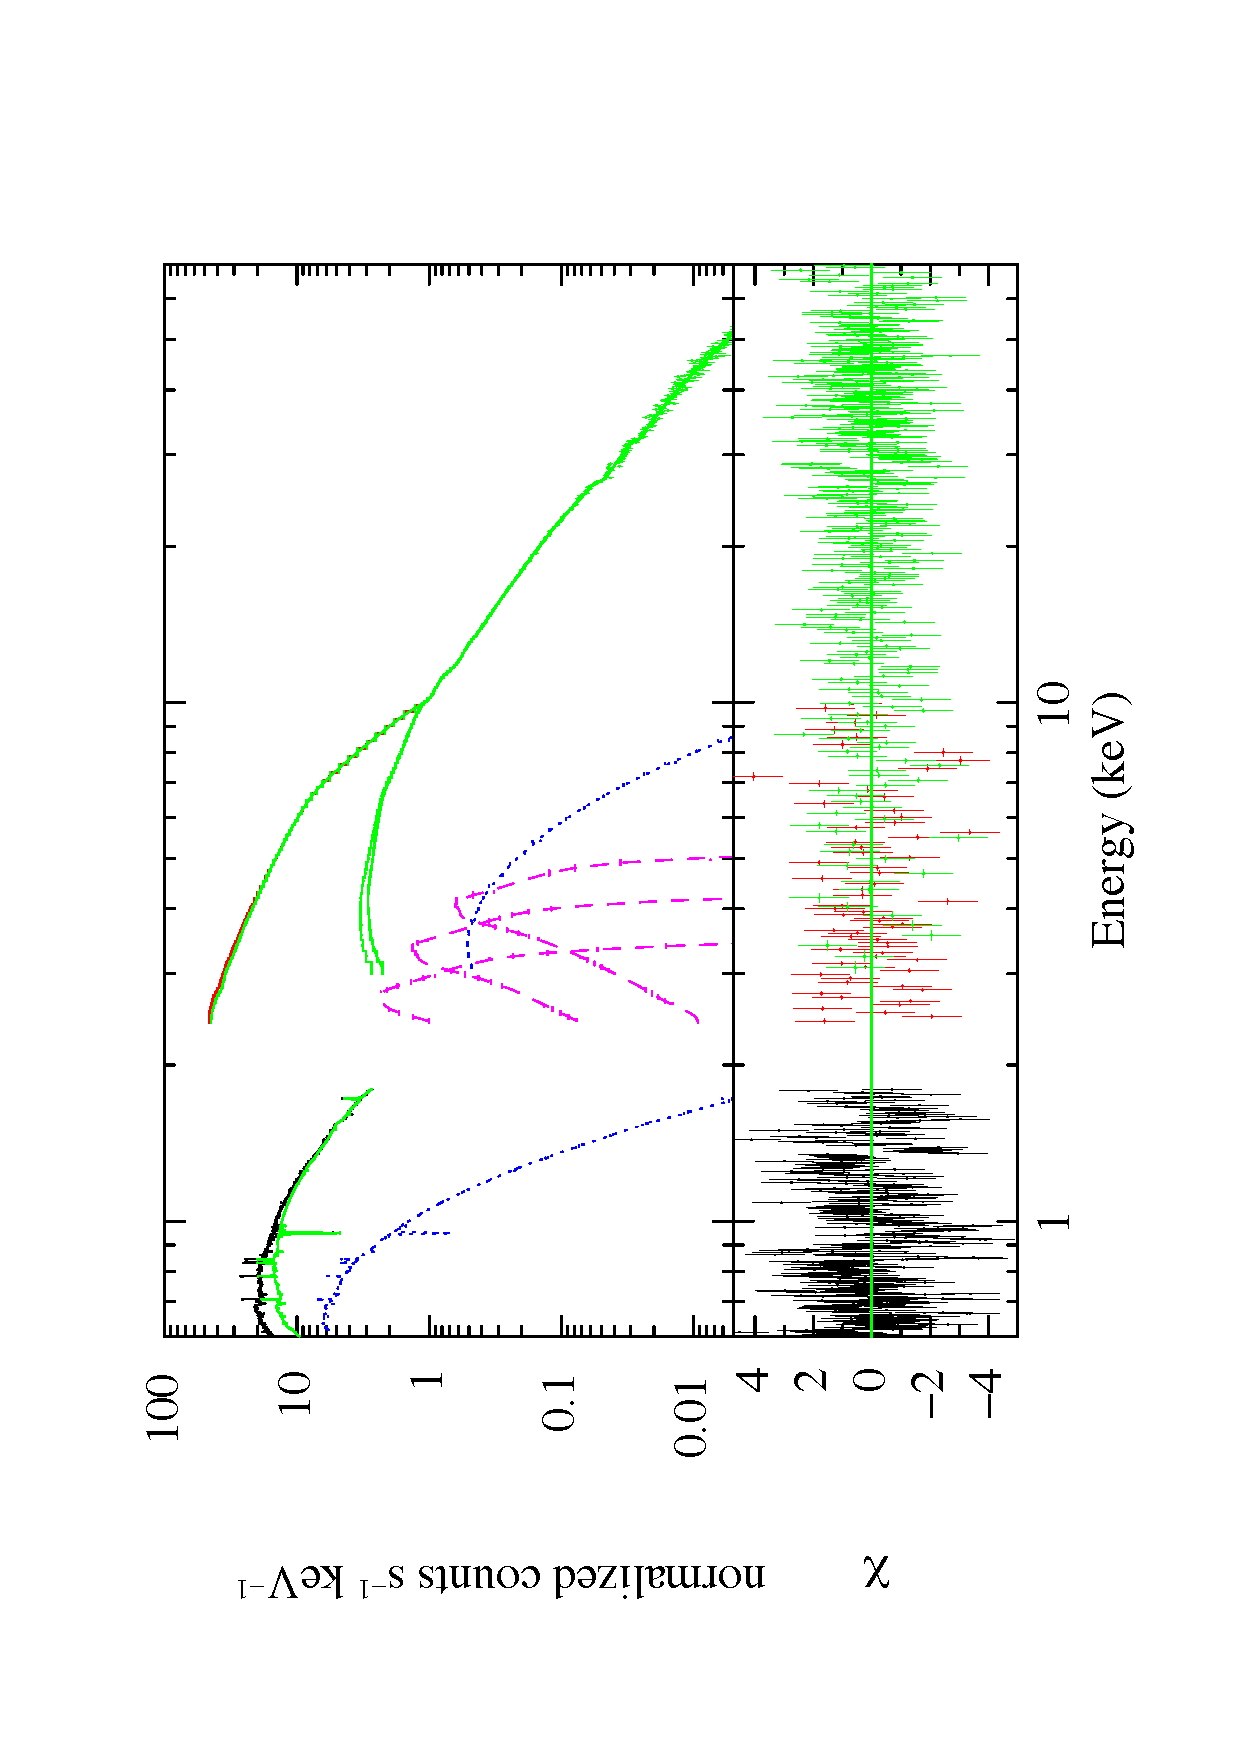
\includegraphics[width=1.0\linewidth]{REVIEW_AMXP/nus_xmm_relxill_diskl_new}
  \label{fig:sfig1}
\end{subfigure}%
\begin{subfigure}{.5\textwidth}
  \centering
  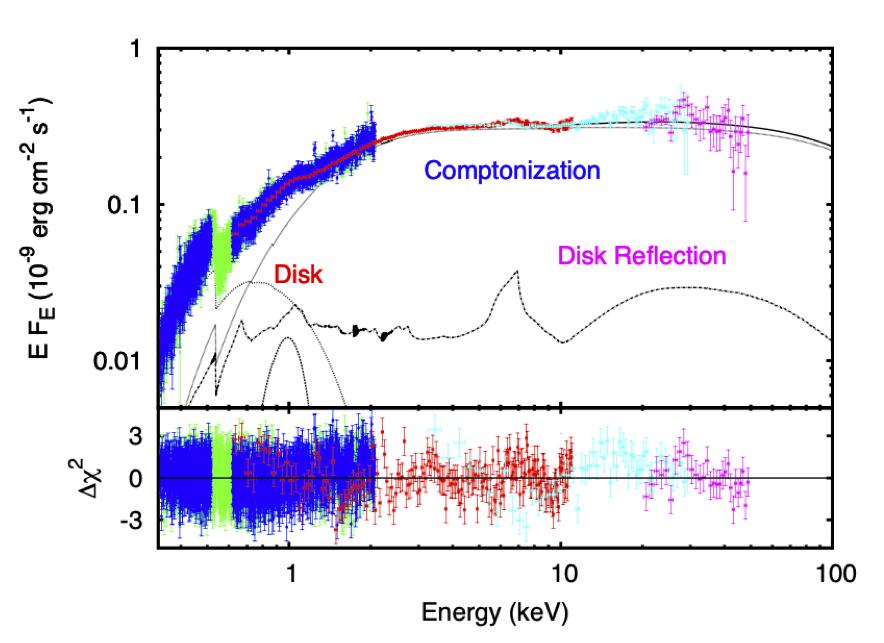
\includegraphics[width=1.0\linewidth]{REVIEW_AMXP/hete_spec_croped.png}
  \label{fig:sfig2}
\end{subfigure}
\caption{\textit{Left Panel:} Spectral properties of the AMXP \saxj{} during its 2015 outburst as observed by \xmm{} (black and red points) and \nustar{} (green points). \textit{Right Panel:} Spectral properties of the AMXP HETE J1900.1-2455 in outburst as observed by \xmm{} (blue, green and red points) and \rxte{} (cyan and magenta points).[Figures from \cite{DiSalvo2019,Papitto2013a}]}
\label{fig:spec}
\end{figure}





The (intermittent) AMXP SAX J1748.9-2021, observed by \xmm{} for $\sim 115$ ks and \inte{} \cite{Pintore2016}, was caught at a relatively high luminosity of $\sim 5 \times 10^{37}$ erg/s corresponding to $\sim 25\%$ of the Eddington limit for a $1.4\, M_\odot$ NS, and, exceptionally for an AMXP, showed a spectrum compatible with a soft state. The broad-band spectrum is in fact dominated by a cold thermal Comptonization component (electron temperature of $\sim 2$ keV) with an additional hard X-ray emission described by a power-law (photon index $\Gamma \sim 2.3$), typically detected in LMXBs in the soft state (see e.g. \cite{DiSalvo2000}). In addition, a number of broad (Gaussian $\sigma = 0.1 - 0.4$ keV) emission features, likely associated to reflection processes, have been observed in the \xmm{} spectrum. A broad iron line was observed at an energy of $\sim 6.7-6.8$ keV, consistent with a Fe XXV K$\alpha$ transition produced in the disc at a distance of $\sim 20-43\, R_g$ ($\sim 42 - 90$ km), with an inclination angle of $\sim 38-45^\circ$. The other broad emission lines may be associated to K-shell emission of S XVI (2.62 keV), Ar XVIII (3.32 keV) and Ca XX or Ca XIX (4.11 keV or 3.90 keV, respectively), and are compatible with coming from the same emission region as the iron line. 

High-quality X-ray spectra of \saxj{} were obtained during the 2008 outburst with \xmm{} \cite{Papitto2009} and \suzaku{} \cite{Cackett2009} and during the 2015 outburst with \xmm{} (which observed the source at the peak of the outburst) and \nustar{} which observed the source four days later \cite{DiSalvo2019}. The 2015 spectrum of \saxj{} taken with \nustar{} was quite similar to the 2008 spectra; the continuum emission was modelled with one or two blackbody-like components and a hard Comptonization component with an electron temperature $> 40$ keV. On the other hand, the 2015 \xmm{} spectrum was surprisingly much softer, with an electron temperature below 10 keV and a much colder blackbody component (corresponding to a large radius, $> 100$ km, for the emitting surface, \cite{DiSalvo2019}). 
In all the cases, a reflection component was also required to model both the broad iron line and the Compton hump observed on top of the continuum. All the smearing parameters were quite similar in the 2008 and 2015 spectra, with the exception of the ionization parameter, much higher during the 2015 \xmm{} observation ($\log \xi \sim 3.5$),
%, where $\xi = L_X / n_e r^2$, where $L_X$ is the X-ray luminosity, $n_e$ is the electron density, and $r$ is the distance from the central illuminating source), 
which also showed broad emission lines from highly ionized elements (S XVI, Ar XVIII and Ca XIX-XX). In particular, the inner disk radius was $\sim 10\, R_g$, corresponding to about 20 km; for comparison the co-rotation radius of the system is $31 m_{1.4}^{1/3}$ km, where $m_{1.4}$ is the NS mass in units of $1.4\, M_\odot$, indicating that the disk is truncated inside the co-rotation radius during the outburst, as expected from the observed timing properties of the source. 
%%
However, the inclination angle is required to be high (usually values $> 60^\circ$ are required, the best constraint comes from the 2015 \xmm{} spectrum, where $i = 58^\circ \div 64^\circ$, \cite{DiSalvo2019}). This result is in agreement with evidences from the 2015 \xmm{} spectrum of discrete absorption features, namely an absorption edge at $\sim 7.4$ keV from neutral or mildly ionized iron and at least two absorption lines, possibly from K transitions of highly ionized (He-like) Ne IX (at 0.947 keV) and Mg XI (at 1.372 keV). These lines are relatively broad (implying a velocity dispersion of $\sigma_v \sim 0.01c$) and blue-shifted at a velocity a few percent the speed of light \cite{DiSalvo2019}. If confirmed, these lines may suggest the presence of a weakly relativistic outflowing wind towards the observer. A high inclination angle is also compatible with other estimates (see e.g. \cite{Ibragimov2009,Deloye2008,Bildsten2001,Wang2013}). However, high values for the inclination angle of the system look at odd when considered together with optical estimates of the radial velocity of the companion star \cite{Elebert2008,Cornelisse2009}, since it implies quite low values for the NS mass, $M_{NS} \sim 0.5 \div 0.8\, M_\odot$. These results may indicate some problem with the interpretation of the reflection component and/or the need of more precise measurements of the radial velocity of the companion star. 

It is noteworthy that reflection features are not always observed in AMXPs. Indeed, no evidence of iron emission lines or reflection humps has been reported for IGR J16597-3704 \cite{Sanna2018a} observed by \swift{} and \nustar{}, IGR J17379-3747 \cite{Sanna2018b} observed by \xmm{}, XTE J1807-294 \cite{Falanga2005a} observed by \rxte{}, \xmm{} and \inte{}, and XTE J1751-305 \cite{Miller2003} observed by \xmm{}. Similar results have been reported for the 2018 outburst of the AMXP SWIFT J1756.9-2508 monitored by several satellites such as \nicer{}, \swift{}, \xmm{}, \nustar{} and \inte{}.  Evidences of iron emission lines in the 6-7 keV band have been, however, reported from the analysis of \rxte{} observations of the source during its 2007 and 2009 outbursts \cite{Patruno2010c}.

\subsection{Short-term variations of the spin during outbursts}

Accretion torque theories can be tested studying the spin variations of AMXPs during accretion phases. These studies can provide valuable information on the mass accretion rate and magnetic field of the NS in these systems, as well as their spin evolution. Coherent timing has been performed on several sources of the sample, with sometimes controversial results (see \cite{Campana2018} for a recent review). Some sources seem to show spin-up during outbursts (e.g.\ IGR J00291+5934, XTE J1751-305, XTE J1807-294, IGR J17511-3057), while other sources seem to show spin-down even during accretion phases (e.g. XTE J0929-314,  XTE J1814-338, IGR J17498-2921 and IGR J17591-2342). Although some AMXPs show pulse phase delays distributed along a second order polynomial, indicating an almost constant spin frequency derivative, other sources show strong timing noise (e.g. SAX J1808-3658, HETE 1900-2455), sometimes correlated with sharp variations of the X-ray flux, which can hamper any clear measurement of the spin derivative.

The first AMXP for which a spin derivative has been measured is the fastest spinning ($\sim 599$ Hz, in a 2.46 hr orbit) among these sources, IGR J00291+5934. It is now generally accepted that this source shows spin up at a rate of $\sim (5-8) \times 10^{-13}$ Hz s$^{-1}$ \cite{Falanga2005b,Patruno2010}. \cite{Burderi2007} have attempted to fit the phase delays vs.\ time with physical models taking into account the observed decrease of the X-ray flux as a function of time during the X-ray outburst, with the aim to get a reliable estimate of the mass accretion rate onto the compact object. 
Because the X-ray flux, which is assumed to be a good tracer of the mass accretion rate, is observed to decrease along the outburst, this has to be considered in eq.(\ref{torque}) in order to obtain the correct value of the mass accretion rate, and hence of the spin frequency derivative, at the beginning of the outburst as well as its variation during the outburst. This approach has been successfully applied to the timing of the 2014 outburst of the so-called {\it bursting pulsar}, GRO J1744-28, an X-ray pulsar with a spin frequency of $2.14$ Hz in a $11.83$ days orbit around a $0.2\, M_\odot$ companion star. \cite{Sanna2017b} were able in this way to obtain a good fit of the pulse phase delays versus time, deriving a frequency spin-up of $\sim 9 \times 10^{-12}$ Hz/s and inferring a distance to the source between 3.4 and 4.1 kpc, assuming a disk viscous parameter $\alpha$ in the range of 0.1-1.   
In the case of IGR J00291+5934, this technique gives a spin frequency derivative at the beginning of the outburst of $\dot \nu \sim 1.2(2) \times 10^{-12}$ Hz s$^{-1}$, corresponding to a mass accretion rate of $\sim 7 \times 10^{-9}\, M_\odot/yr$ and a peak bolometric luminosity of $\sim 7 \times 10^{37}$ erg/s for the 2004 outburst. This is at least one order of magnitude higher than the X-ray luminosity inferred from the observed X-ray flux, assuming a distance of 4.2 kpc. Once we will have a direct, independent, estimate of the distance to the source, we will have the possibility to test the $\dot M$ vs.\ X-ray luminosity relation, torque theories and/or the physical parameters of the NS in this system. 

A recent example of an AMXP showing spin-down while accreting is given by IGR J17591--2342. This source has been extensively monitored by \nicer{} during its outburst starting from 2018 August 15 up to 2018 October 17 for a total exposure time of  $\sim101$ ks distributed into 37 dedicated observations. X-ray pulsations have been detected uninterruptedly for almost 60 days allowing to accurately investigate the NS spin frequency evolution. Phase-coherent timing analysis of the frequency fundamental and first harmonic components revealed a statistically significant negative frequency derivative $\dot{\nu}\sim -7\times 10^{-14}$ Hz/s \cite{Sanna2020c} (see however, \cite{Kuiper2020} for different results from the timing analysis). Further analysis of the the X-ray pulse phase evolution of IGR J17591--2342, adopting a physical model that accounts for the accretion material torque as well as the magnetic threading of the accretion disc in regions where the Keplerian velocity is slower than the magnetosphere velocity, allows to constrain the NS magnetic field to be $B_{eq} = 2.8(3)\times10^8$ G \cite{Sanna2020c}.

A similar spin frequency evolution has been reported for the AMXPs IGR J17498-2921 ($\dot{\nu} -6.3(1.9)\times 10^{-14}$ Hz/s \cite{Papitto2011b}), XTE J1814-338 ($\dot{\nu} -6.7(7)\times 10^{-14}$ Hz/s \cite{Papitto2007}), and XTE J0929-314 ($\dot{\nu} -9.2(4)\times 10^{-14}$ Hz/s \cite{Galloway2002}). %and SAX J1808.4-3658 for which evidences of a spin-down derivative have been reported during the decay phase of its 2002 outburst ($\dot{\nu}=-7.6(1.5)\times 10^{-14}$ Hz s$^{-1}$ \cite{Burderi2006}) and during its 2019 outburst ($\dot{\nu}=-3.0(1)\times 10^{-13}$ Hz s$^{-1}$ \cite{Bult2019c}, see, however, the discussion for possible different interpretations of this result). 
These observations indicate that spin-down during accretion phases is possible and requires a magnetic threading of the accretion disk.  

The best studied, as well as most discussed source, is certainly the first discovered AMXP, SAX J1808-3658. Differently from all the other AMXPs, this source shows X-ray outbursts almost regularly every $2-4$ years. To date we have observed (with instruments with high-time resolution capabilities) eight outbursts from this source, each lasting about one month. The pulse phase evolution during the outburst shows a strong timing noise, with phases going up and down without any clear correlation with flux variations, or remaining constant for a long time before jumping to another constant phase value (see e.g. \cite{Hartman2008,Hartman2009a, Hartman2009b}). In the attempt to gain information on the spin variations in this source, \cite{Burderi2006} have analysed separately the fundamental and first harmonic of the pulse profile during the 2002 outburst of the source, finding that while the phases of the fundamental are dominated by timing noise, the first harmonic shows a more regular behaviour. This suggests that the phase jump in the fundamental is not related to an intrinsic spin variation (which would have affected the whole pulse profile), but is instead caused by a change of the shape of the pulse profile, leaving the possibility that the harmonic is a better tracer of the NS spin. A similar behavior of the first harmonic has also been observed in other AMXPs (e.g. \cite{Riggio2008,Riggio2011,Papitto2012}).  Under this hypothesis, the fitting of the first harmonic phase delays reveals a spin-up at the beginning of the outburst of $\dot \nu = 4.4(8) \times 10^{-13}$ Hz s$^{-1}$, corresponding to a mass accretion rate of $\dot M \sim 1.8 \times 10^{-9}\, M_\odot$ yr$^{-1}$, and a constant spin-down, of $\dot \nu_{sp} = 7.6(1.5) \times 10^{-14}$ Hz s$^{-1}$, dominating the phase delays at the end of the outburst. The mass accretion rate inferred from timing is only a factor of 2 larger than the observed X-ray luminosity at the beginning of the outburst, that is $\sim 10^{37}$ ergs s$^{-1}$. The spin-down can be interpreted in terms of the threading of the accretion disk by the NS magnetic field outside the co-rotation radius, which, in agreement with expectations, appears to be more relevant at the end of the outburst, when the mass accretion rate significantly decreases. The derived magnetic field, $B = (3.5 \pm 0.5) \times 10^8$ G, is perfectly in agreement with other, independent, constraints (see \cite{Burderi2006}, and references therein).


\begin{figure}
\begin{subfigure}{.5\textwidth}
  \centering
  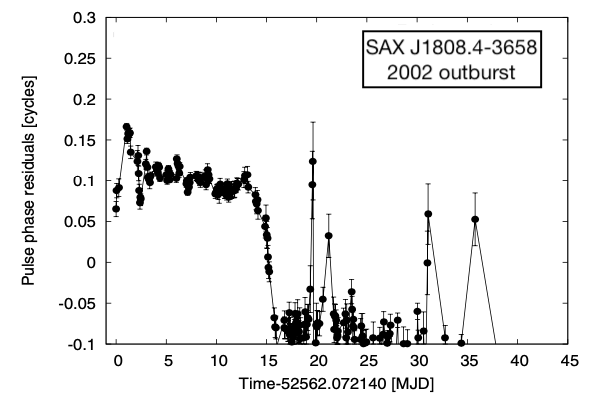
\includegraphics[width=.8\linewidth]{REVIEW_AMXP/1808_phases}
  \label{fig:sfig1}
\end{subfigure}%
\begin{subfigure}{.5\textwidth}
  \centering
  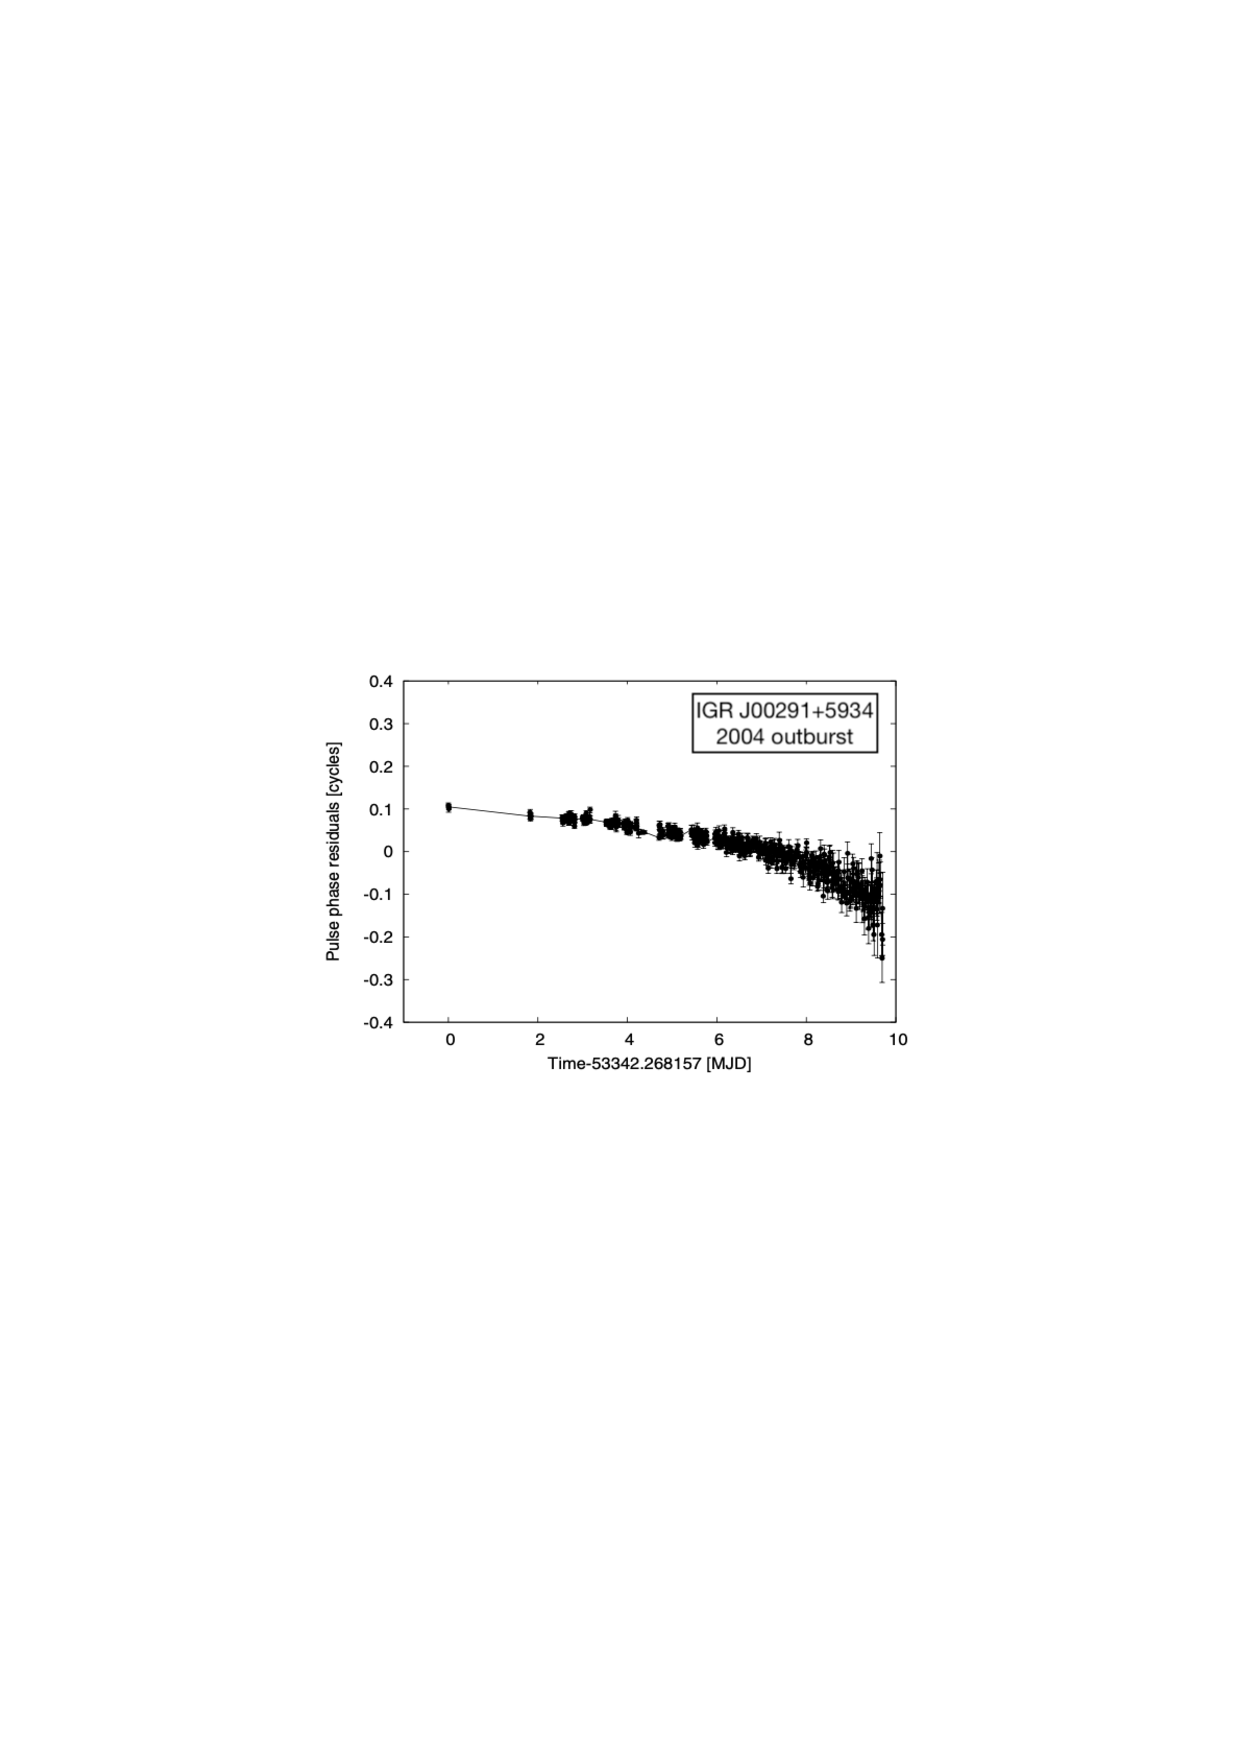
\includegraphics[width=0.9\linewidth]{REVIEW_AMXP/00291_phases_2}
  \label{fig:sfig2}
\end{subfigure}
\caption{Phase residuals of the fundamental frequency for the AMXP \saxj{} (left Panel) and IGR J00291+5934 (right Panel) [Figure adapted from \cite{Patruno2009d}]}
\label{fig:tim_noise}
\end{figure}




The latest outburst of SAX J1808-3658 in 2019 was monitored with NICER for one month and a total exposure of 355.4 ks. Timing analysis of these data showed that the pulse profile was dominated by the fundamental (the first harmonic was significantly detected only in a handful of intervals) and the relative phase delays show a clear parabolic trend typical of a spin-down at the rate of $\dot{\nu} = -3.02(13)\times 10^{-13}$ Hz s$^{-1}$ \cite{Bult2019c}. Since these phase shifts appear to be correlated with the source flux, the authors interpreted this trend in terms of hot-spot drifts on the stellar surface, driven by changes in the mass accretion rate.    

Other recent results regard phase-coherent timing analysis of the outburst of the AMXPs SWIFT J1759-2508 and IGR J17379-3737, which allowed to set upper limits on the spin frequency derivative of $\dot{\nu}<|1.4|\times 10^{-12}$ Hz/s \cite{Sanna2019,Bult2018b} and $-0.5\times 10^{-14}<\dot{\nu}<0.9\times 10^{-14}$ Hz/s \cite{Bult2019c}, respectively.



\subsection{Long-term variations of the spin}
%\textbf{J1808; IGR J00291 (2015)}
AMXPs for which more than one outburst has been observed with high time resolution instruments, allow to derive long term spin evolution comparing the averaged spin frequency measured in each outburst. To date only six AMXPs have been observed in different outbursts: SAX J1808.4--3658, IGR J00291+5934, XTE J1751--305, Swift J1756.9--2508, IGR J17379--3747, IGR J17511--3057, NGC 6440 X--2, and SAX J1748.9--2021 (although, with relatively low S/N and short outburst duration for some of these sources, see Table \ref{Tab2}). 

The best constrained long-term spin evolution is obtained for \saxj{} (\textbf{left panel of Fig.~\ref{fig:1808_sec},}), for which secular spin evolution has been measured over a 13 year time span (between 1998 and 2011), which shows a constant long-term spin-down at a rate of $\sim -1 \times 10^{-15}$ Hz s$^{-1}$ (see \cite{Patruno2012}, and references therein). Because of the stability of the spin-down rate over the years, the most likely explanation appears to be loss of angular momentum via magnetic-dipole radiation, which is expected for a rapidly rotating NS with a magnetic field. The measured spin-down is consistent with a polar magnetic field of $(1.5 - 2.5) \times 10^8$ G, in agreement with other estimates. The spin frequency measured during the 2015 outburst had a large uncertainty because of strong timing noise of the fundamental. Interestingly, the spin frequency measured using the phases of the first harmonic falls very close (less than $2 \sigma$) from the value predicted by the secular evolution (see \cite{Sanna2017c}). For the 2019 outburst, the first harmonic is significantly detected only in few \nicer{} snapshots and the exact value of the spin frequency inferred from the fundamental depends on the adopted timing solution. \cite{Bult2019c} have fitted the phase delays using a linear model (which leaves large residuals), a quadratic model (indicating a spin-down during the outburst), and a flux-adjusted model (under the hypothesis that phase variations with time originate from a hot-spot drifting on the stellar surface, driven by changes in the mass accretion rate). The linear and flux-adjusted models give a spin frequency relatively close to the secular spin-down trend, while the quadratic model gives a frequency lying significantly above the trend. Considering the linear model (which provides the frequency value closest to the expected trend), the long-term evolution of the spin shows a modulation around a constant spin-down behaviour at the Earth's orbital period (\textbf{right panel of Fig.~\ref{fig:1808_sec},}), which is used to astrometrically refine the source coordinates.


\begin{figure}
\begin{subfigure}{.5\textwidth}
  \centering
  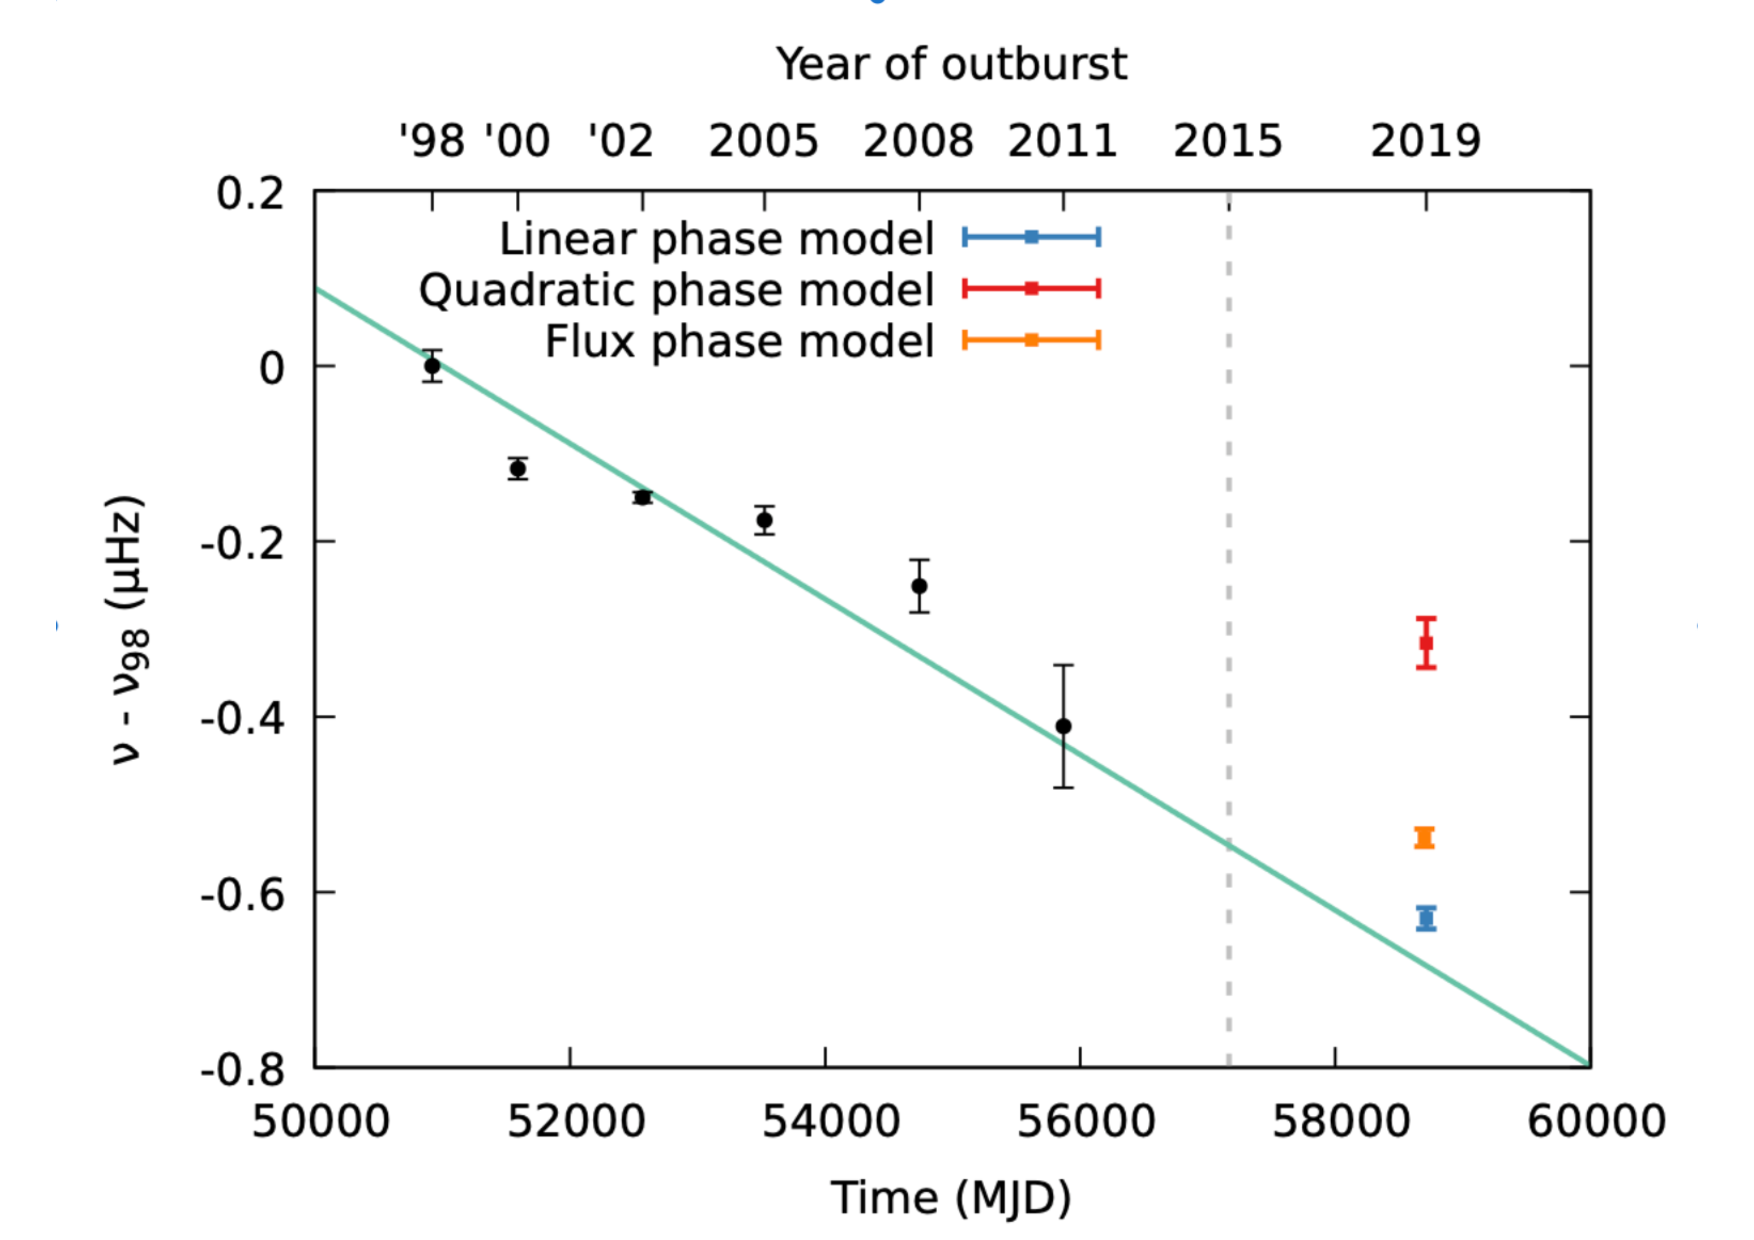
\includegraphics[width=.8\linewidth]{REVIEW_AMXP/1808_secular_3}
  \label{fig:sfig1}
\end{subfigure}%
\begin{subfigure}{.5\textwidth}
  \centering
  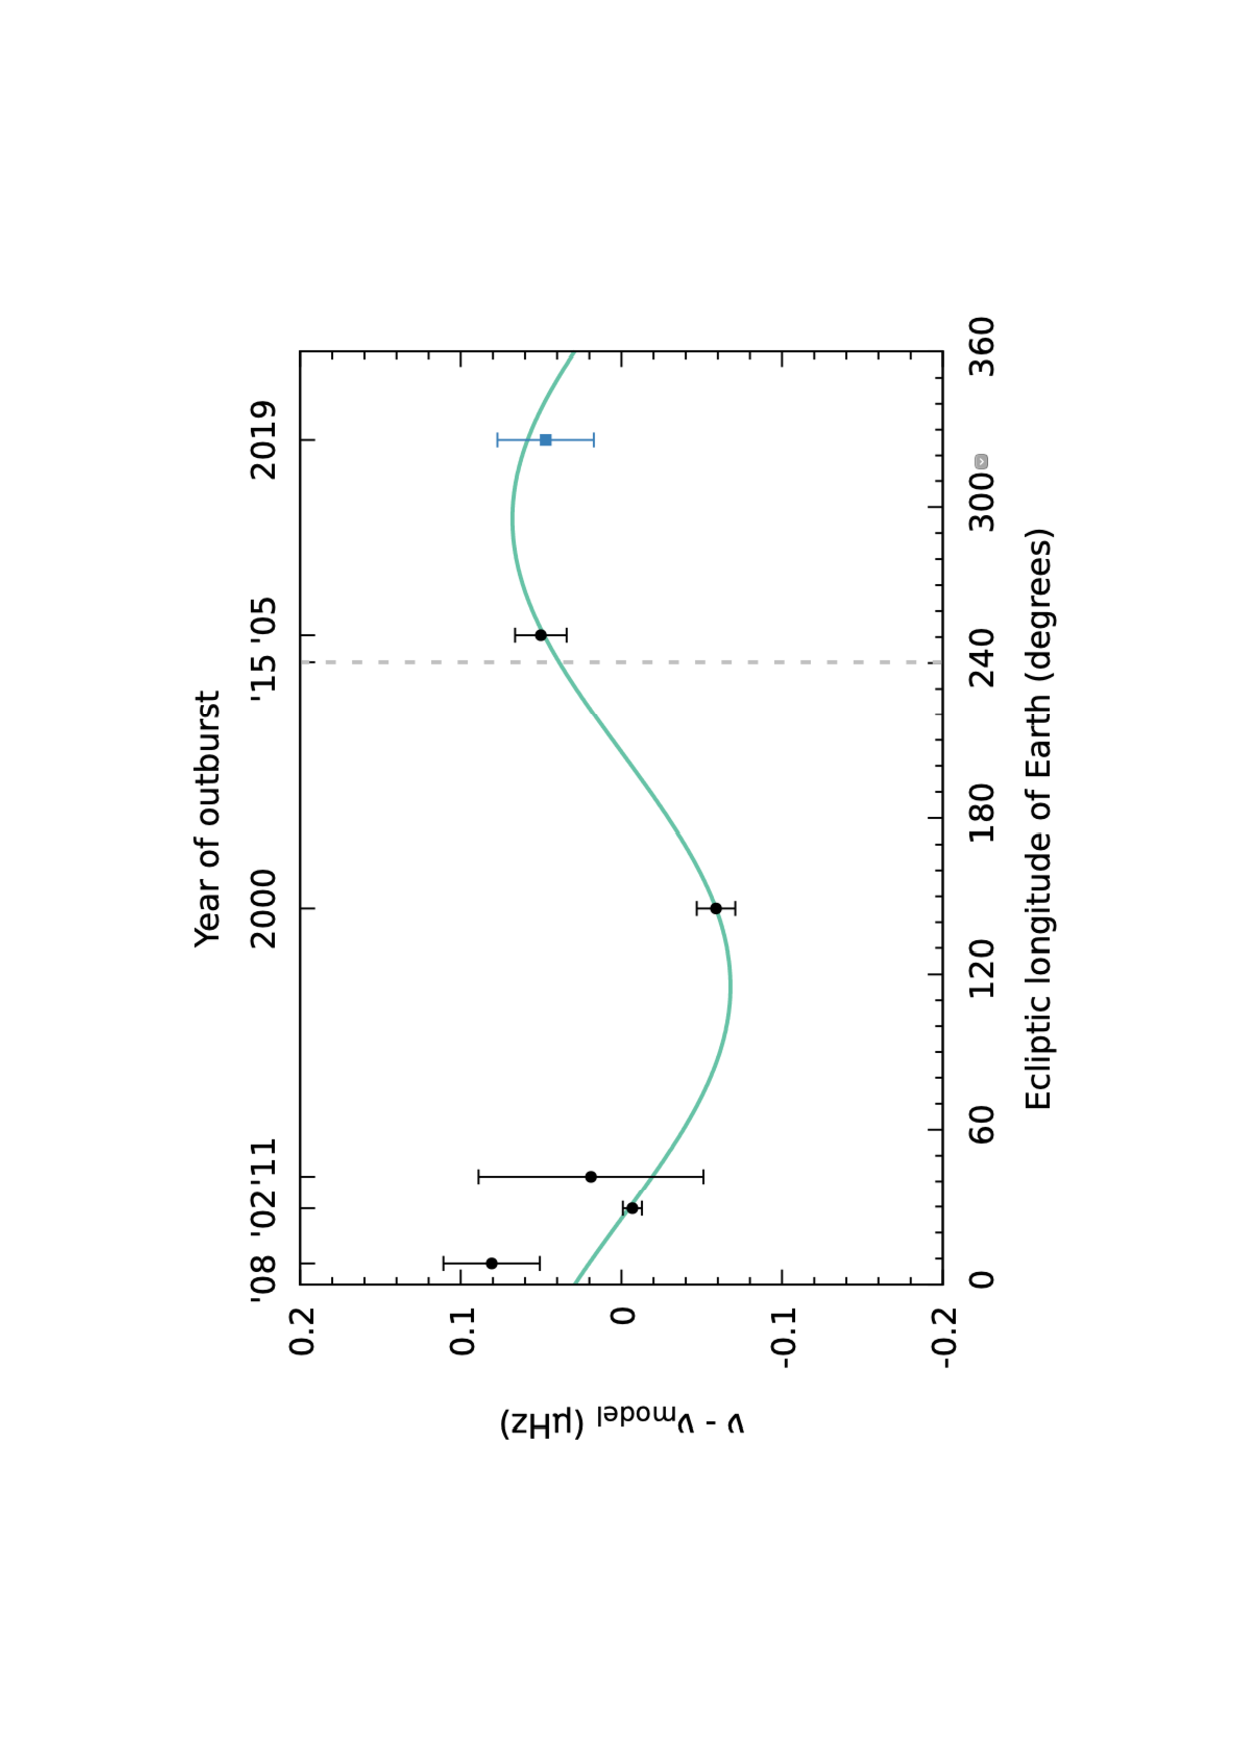
\includegraphics[angle=-90,width=1.1\linewidth]{REVIEW_AMXP/1808_new_pos}
  \label{fig:sfig2}
\end{subfigure}
\caption{\textit{Left Panel:} Secular spin frequency evolution of the AMXP \saxj{} calculated relatively to the 1998 epoch. Black points represent measurements obtained with \rxte{} while colored squared represent the \nicer{} measurements obtained for the 2019 outburst of the source for three different models (see \cite{Bult2019c} for more details). The solid line indicates the spin evolution best fit model. \textit{Right Panel:} Spin frequency measurements f the AMXP \saxj{} relative to the best-fit spin-down model as a function of the Earth's ecliptic longitude. [Figure from \cite{Bult2019c}]}
\label{fig:1808_sec}
\end{figure}





\begin{comment}
\begin{figure}
\centering
  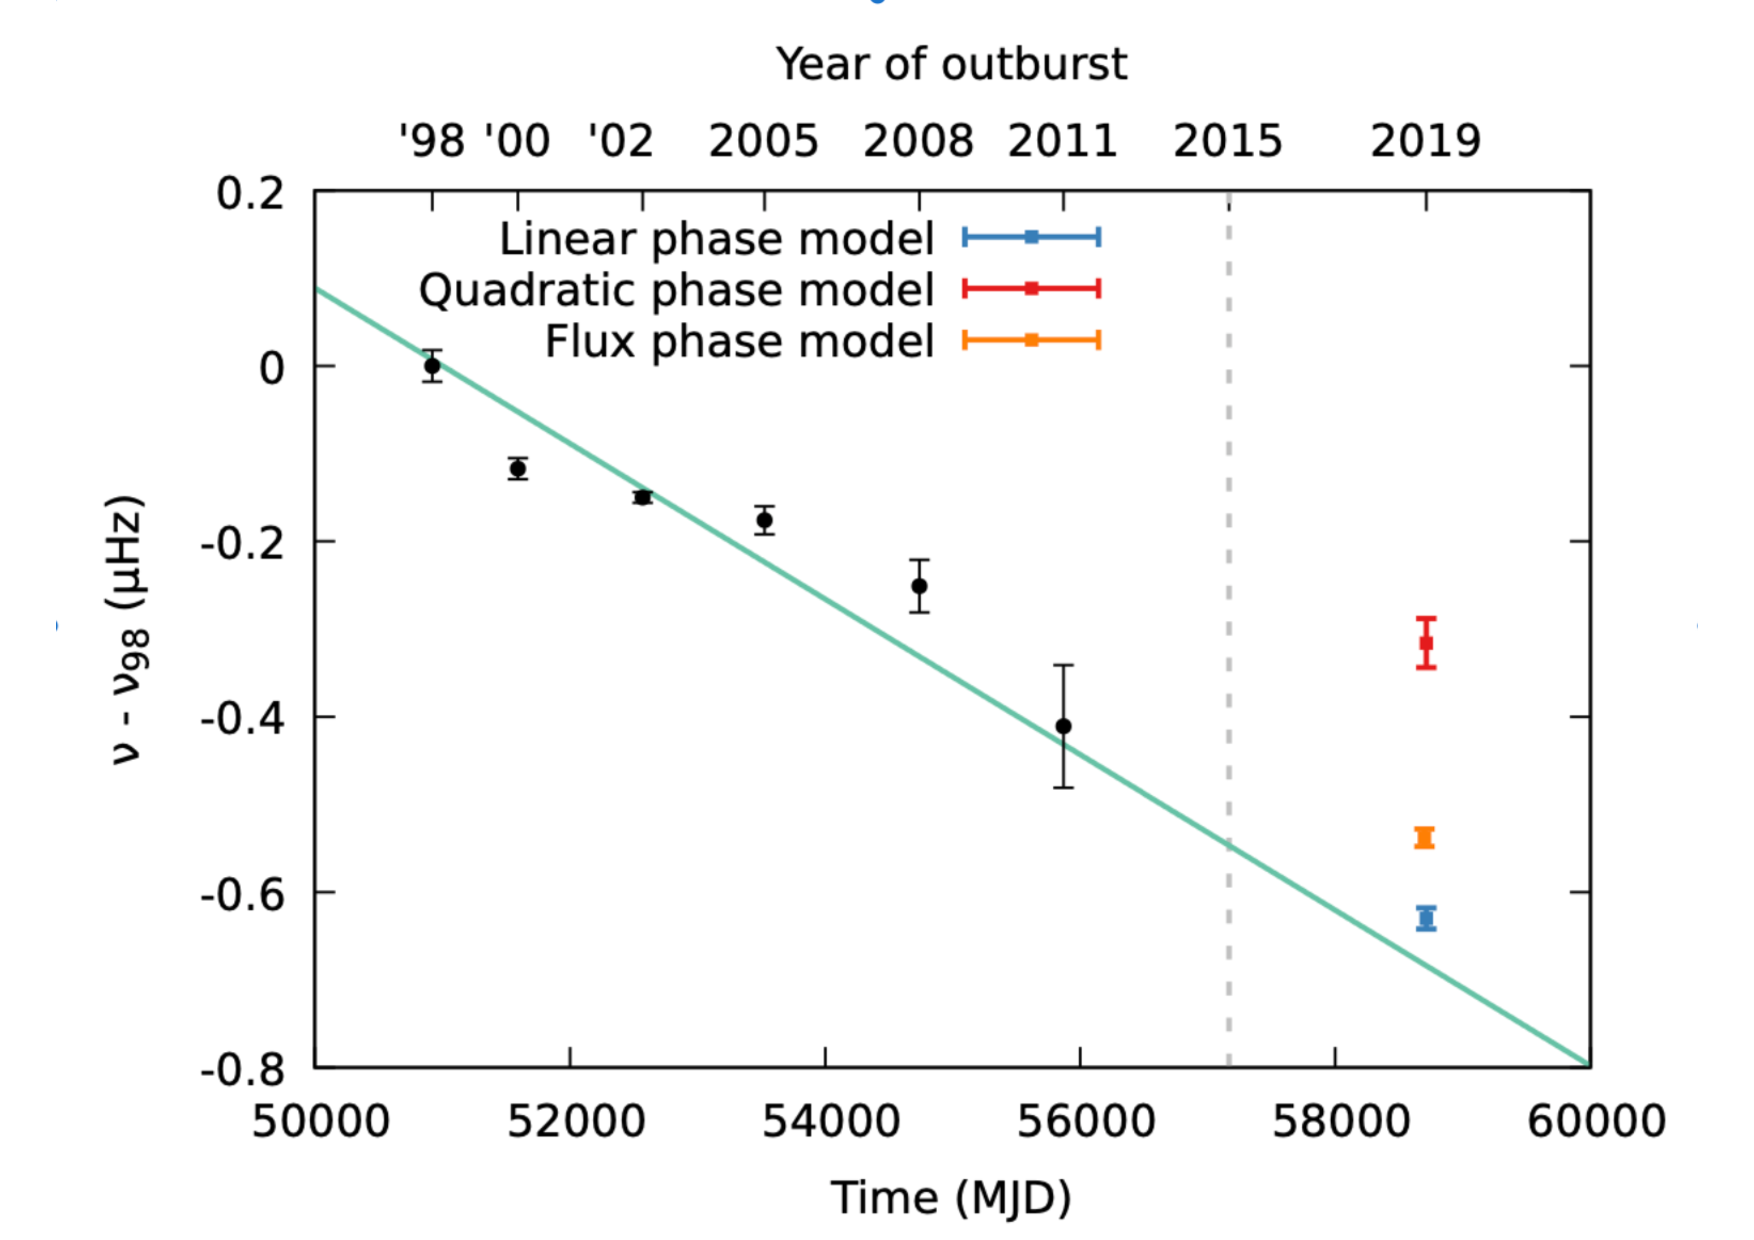
\includegraphics[width=0.55\textwidth]{REVIEW_AMXP/1808_secular_3}
  \caption{ [Figure from \cite{Bult2019c}}     
  \label{fig:lc_0911}
\end{figure}
\end{comment}


A long-term spin-down has also been measured for IGR J00291+5934 between the 2004 and 2008 outbursts, at a rate of $-4.1(1.2) \times 10^{-15}$ Hz s$^{-1}$, larger than that observed in \saxj{}, as expected given that IGR J00291+5934 spins at a higher frequency. Including the 2015 outburst, the long-term spin-down becomes $|\dot{\nu}|< 6\times 10^{-15}$ Hz s$^{-1}$  (see \cite{Sanna2017d} and references therein). If interpreted in terms of magneto-dipole emission, the measured spin-down translates into an estimate of the NS magnetic field of $(1.5-2) \times 10^8$ G. Another possibility is given by the spin-down torque associated with the emission of GR, strongly dependent on the NS spin, which has also been proposed as a limiting factor for the maximum spin frequency observed for a NS (to date 716 Hz, \cite{Hessels2006}). Assuming that the long-term spin-down observed in IGR J00291+5934, the fastest spinning AMXP known to date, is due to this mechanism, the measurement of the average spin-down in this source translates to an upper limit on the average mass quadrupole moment of $Q \lesssim 2 \times 10^{36}$ g cm$^2$ \cite{Hartman2011}. Under this hypothesis, it is possible to predict that the long-term spin-down in IGR J00291+5934 should be a factor 7.6 higher than in \saxj{}. The large uncertainties on these measurements prevent at the moment to assess this prediction, but it can be checked with future, high-quality, monitoring of the spin frequency in these systems.

Long-term spin evolution has been constrained for a few other sources of the sample of AMXPs. After the discovery of X-ray pulsations during the 2018 outburst of IGR J17379--374, pulsations from this source have been discovered also in the \rxte{} archival data of its 2004 and 2008 outbursts after applying the binary ephemeris. Combining the barycentric spin frequency values from the three oubursts, an upper limit on the secular spin derivative has been estimated, $-8.3\times10^{-13}$ Hz/s $<\dot{\nu}<1.1\times 10^{-12}$ Hz/s. This corresponds to an upper limit on the magnetic field strength of $B<2.8\times 10^9$ G, under the assumption of a NS radius of 10 km and an angle $\alpha\simeq 10^\circ$ between the magnetic hotspot and the rotational pole \cite{Sanna2018b}. Swift J1756.9--2508 has been detected in outburst three times (2007, 2009 and 2018) since its discovery, which allowed the detection of a long-term spin-down derivative of $-4.8(6)\times 10^{-16}$ Hz/s \cite{Sanna2019}, corresponding to a NS superficial magnetic field $1.5\times 10^8 < B_{eq} < 2.2\times 10^8$ G (consistent with the value reported by \cite{Mukherjee2015}).
 

\subsection{Long-term timing of the orbital period}
The study of the orbital evolution in Low Mass X-ray Binary systems is very important to constrain the evolutionary path leading to the formation of rotation-powered MSPs, and hence to obtain information on the progenitors of fast-rotating NS and on the recycling scenario. In principle, it can also put constraints on alternative theories of Gravity. In fact, since the difference in the orbital period evolution of binaries interpreted with General Relativity (GR) and other theories of Gravity (e.g. Brans-Dicke gravity) is related to the mass difference of the two members of the binary system \cite{Will2006}, these sources provide prime candidates for constraining deviations from GR \cite{Psaltis2008}. In this framework, AMXPs are the most promising candidates for an experimental test on these alternative theories, because the companion star is, in most cases, a very light white dwarf or even a brown dwarf \cite{Bildsten2001}, and the primary stars are millisecond pulsars with orbital periods accurately determined. 
 
However, these studies require a large baseline (tens of years) of data to be able to constraint the orbital period derivative. Hence, one of the main difficulty is given by the limited number of AMXPs observed recurrently into X-ray outburst. To date, only eight AMXPs have more than one outburst observed with high-time resolution instruments since their discovery, and therefore only few constraints on the orbital period derivative have been derived to date (see Table \ref{Tab2}). Moreover, long-term orbital solutions show sometimes residuals that are complex and difficult to interpret. Understanding these complex orbital residuals is therefore of fundamental importance, since it would allow to constrain the orbital period evolution in these systems, providing a way to study the evolutionary path leading to the formation of MSPs. Furthermore, the precise determination of the orbital period derivative caused by mass transfer may give in perspective the possibility to constrain alternative theories of Gravity.

The best constraint on the orbital evolution of AMXPs comes again from \saxj{}, which has shown eight X-ray outbursts to date, allowing to follow its orbital period over 21 years. \textbf{As reported in the left panel of Fig.~\ref{fig:orb_evo},} for each outburst the time of passage of the NS through the ascending node ($T^*$, which is the most sensitive parameter to variations of the orbital period) can be derived and plotted versus time. The orbital residuals (with respect to a constant orbital period) were dominated by a clear parabolic trend up to the 2015 outburst, with residuals with respect to this trend of the order of few seconds \cite{Sanna2017c}. Interpreting this parabolic trend as a constant orbital period derivative, the best-fit value is $\dot P_{orb} = 3.6(4) \times 10^{-12}$ s s$^{-1}$, implying a strong orbital expansion. The origin of the observed $\dot P_{orb}$ is still not fully understood, yet, and different possible mechanisms have been proposed over the years (see e.g. \cite{DiSalvo2008,Hartman2008,Burderi2009,Patruno2012b,Patruno2016}. However, there is consensus on the fact that conservative mass transfer is not compatible with the observed value of $\dot P_{orb}$ for \saxj{}. This can be easily demonstrated by estimating the mass-loss rate from the secondary star as a function of the observed orbital period derivative (see e.g. \cite{Burderi2009}), which implies a mass transfer of the order of $2 \times 10^{-9}\, M_\odot$ yr$^{-1}$. This mass transfer rate is much larger than the mass accretion rate onto the NS, considering that the source accretes matter for about a month every 2-4 yr with a bolometric luminosity at the peak of the outburst barely reaching $10^{37}$ erg s$^{-1}$ (corresponding to a maximum mass accretion rate of $\sim 10^{-9}\, M_\odot$ yr$^{-1}$). The average mass accretion rate over the 17 years from 1998 to 2015 is indeed three orders of magnitude below, $\sim 2 \times 10^{-11}\, M_\odot$ yr$^{-1}$. 

A not conservative mass transfer can explain the large orbital period derivative assuming that the mass transfer rate is $\dot M \sim 10^{-9}\, M_\odot$ yr$^{-1}$, and that most of the transferred matter is expelled from the system with the specific angular momentum at the inner Lagrangian point (see \cite{DiSalvo2008,Burderi2009}). In this case, the non-conservative mass transfer may be a consequence of the so-called \textit{radio-ejection} model, extensively discussed by \cite{Burderi2001}, envisaging that a fraction of the transferred matter in the disc could be swept out by the (radiative and high-energy particles) pressure of the pulsar wind. Alternatively, the large orbital period derivative observed in \saxj{} has been interpreted as the effect of short-term angular momentum exchange between the donor star and the orbit \cite{Hartman2009b,Patruno2012b}, resulting from variations in the spin of the companion star (holding the star out of synchronous rotation) caused by intense magnetic activity driven by the pulsar irradiation, the so-called Applegate \& Shaham mechanism (hereafter A\&S \cite{Applegate1994}). In this case, the orbital period should oscillate, alternating epochs of orbital period increase and decrease, because of the gravitational quadrupole-coupling to the orbit. However, according to this mechanism, the system should evolve to longer orbital periods, because of mass and angular momentum loss, on a timescale of $10^8$ yr (for a 2-hr orbital period and a companion mass of $0.1-0.2\, M_\odot$), thus implying a strong orbital period derivative, similar to that inferred from the quadratic trend observed in \saxj{}. In this framework, the orbital residuals in \saxj{} up to 2015 may be interpreted as small oscillations of few-seconds amplitude caused by the A\&S mechanism superposed on a global orbital period derivative induced by the strong mass-loss from the system \cite{Sanna2017c}. Alternatively, variations of the orbital period with respect to the global parabolic trend may be caused by random fluctuations of the mass transfer (and loss) rate. 

The latest outburst of \saxj{} in 2019, however, shows an abrupt flattening of the parabolic trend \cite{Bult2019c}. Indeed, the measurements between 2008 and 2019 taken alone seem to imply an orbital contraction of the orbit in the last 10 years, with an orbital period derivative of $\dot P_{orb} \simeq -5.2 \times 10^{-12}$ s s$^{-1}$. Alternatively, fitting all the measurements with a global parabolic trend, gives an orbital period derivative of $\dot P_{orb} = 1.6 \pm 0.7 \times 10^{-12}$ s s$^{-1}$. \textbf{As shown in the left panel of Fig.~\ref{fig:orb_evo},} the residuals around this mean trend show a sinusoidal-like, 7-s amplitude, oscillation with a period of approximately 18.2 years. Additional monitoring of future outbursts is needed to confirm the presence of oscillations around a steadily expanding orbit, or, instead, a $\sim 20$ s amplitude modulation around a constant (or much less variable) orbital period.


\begin{figure}
\begin{subfigure}{.5\textwidth}
  \centering
  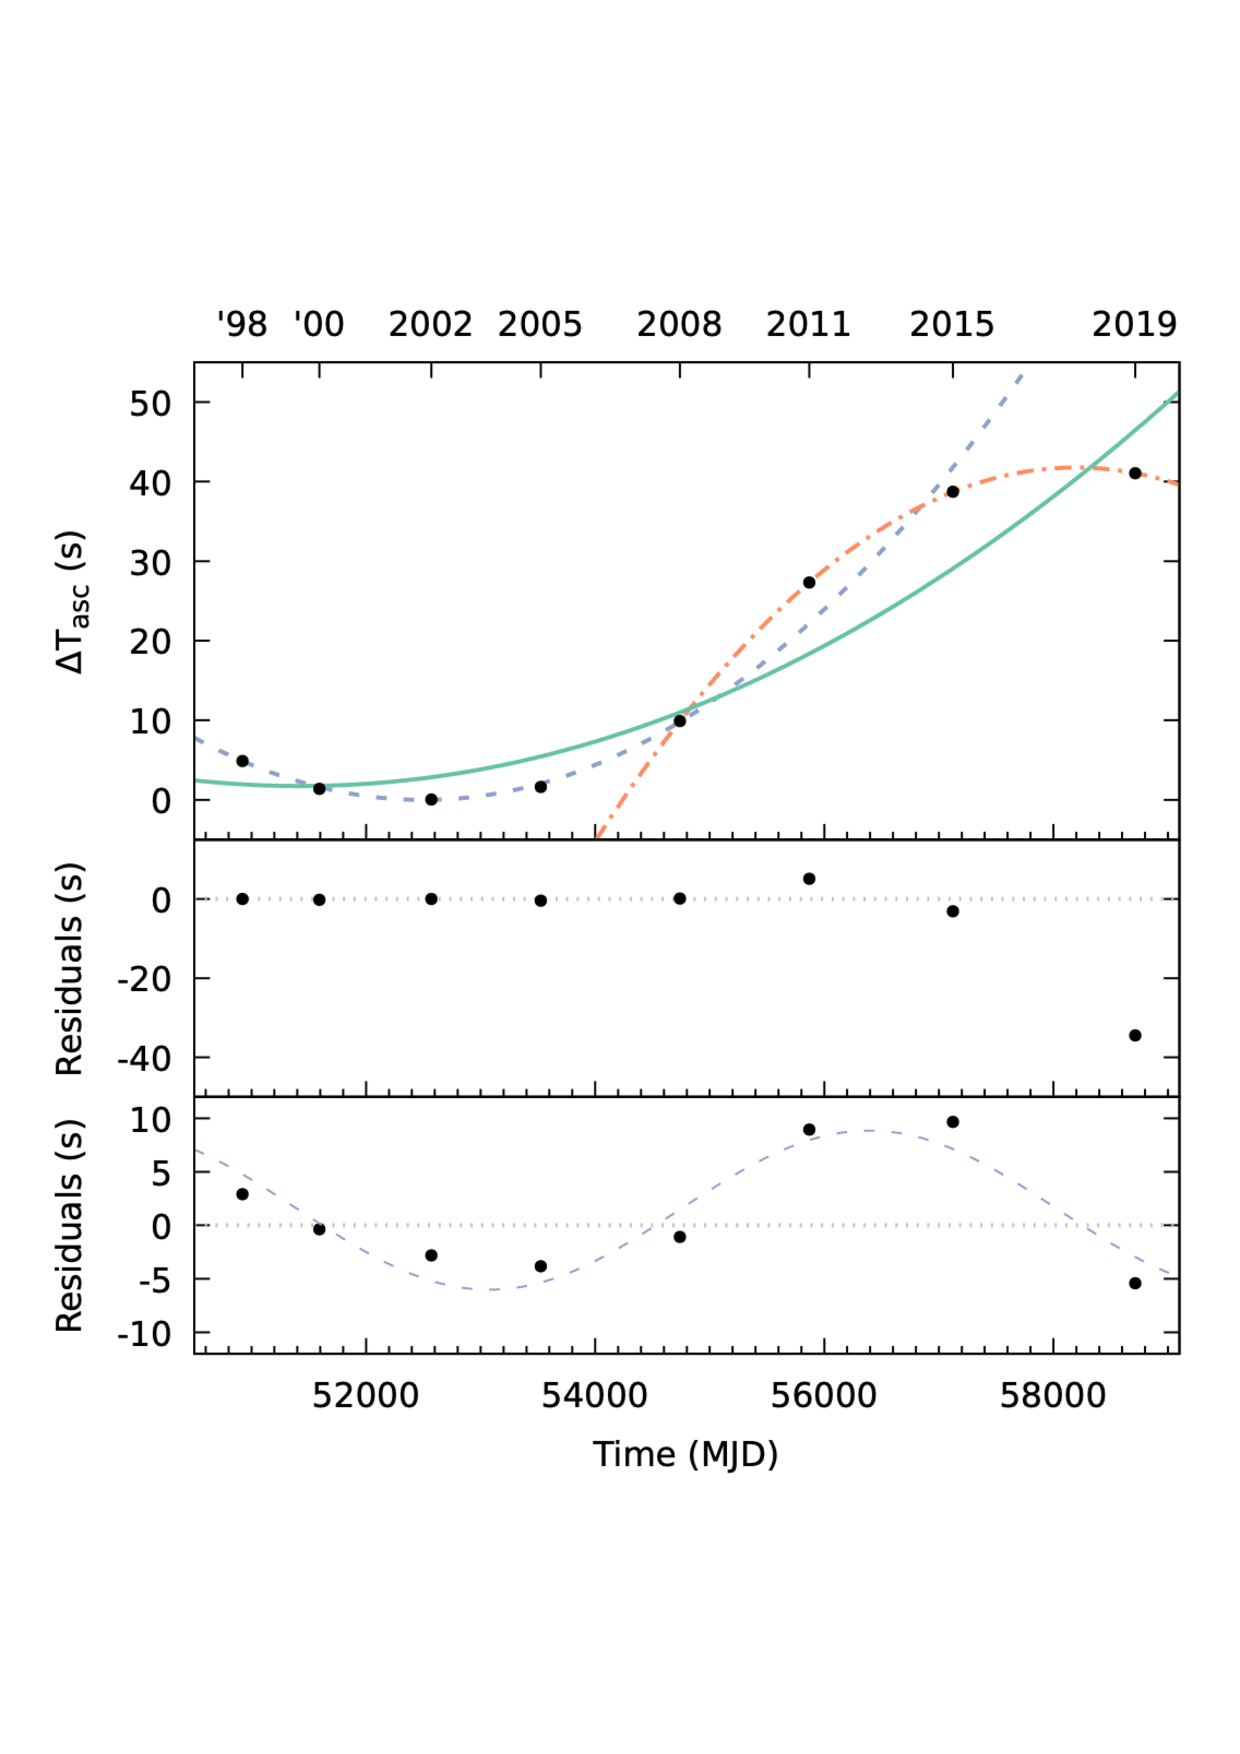
\includegraphics[width=.8\linewidth]{REVIEW_AMXP/1808_orb_2}
  \label{fig:sfig1}
\end{subfigure}%
\begin{subfigure}{.5\textwidth}
  \centering
  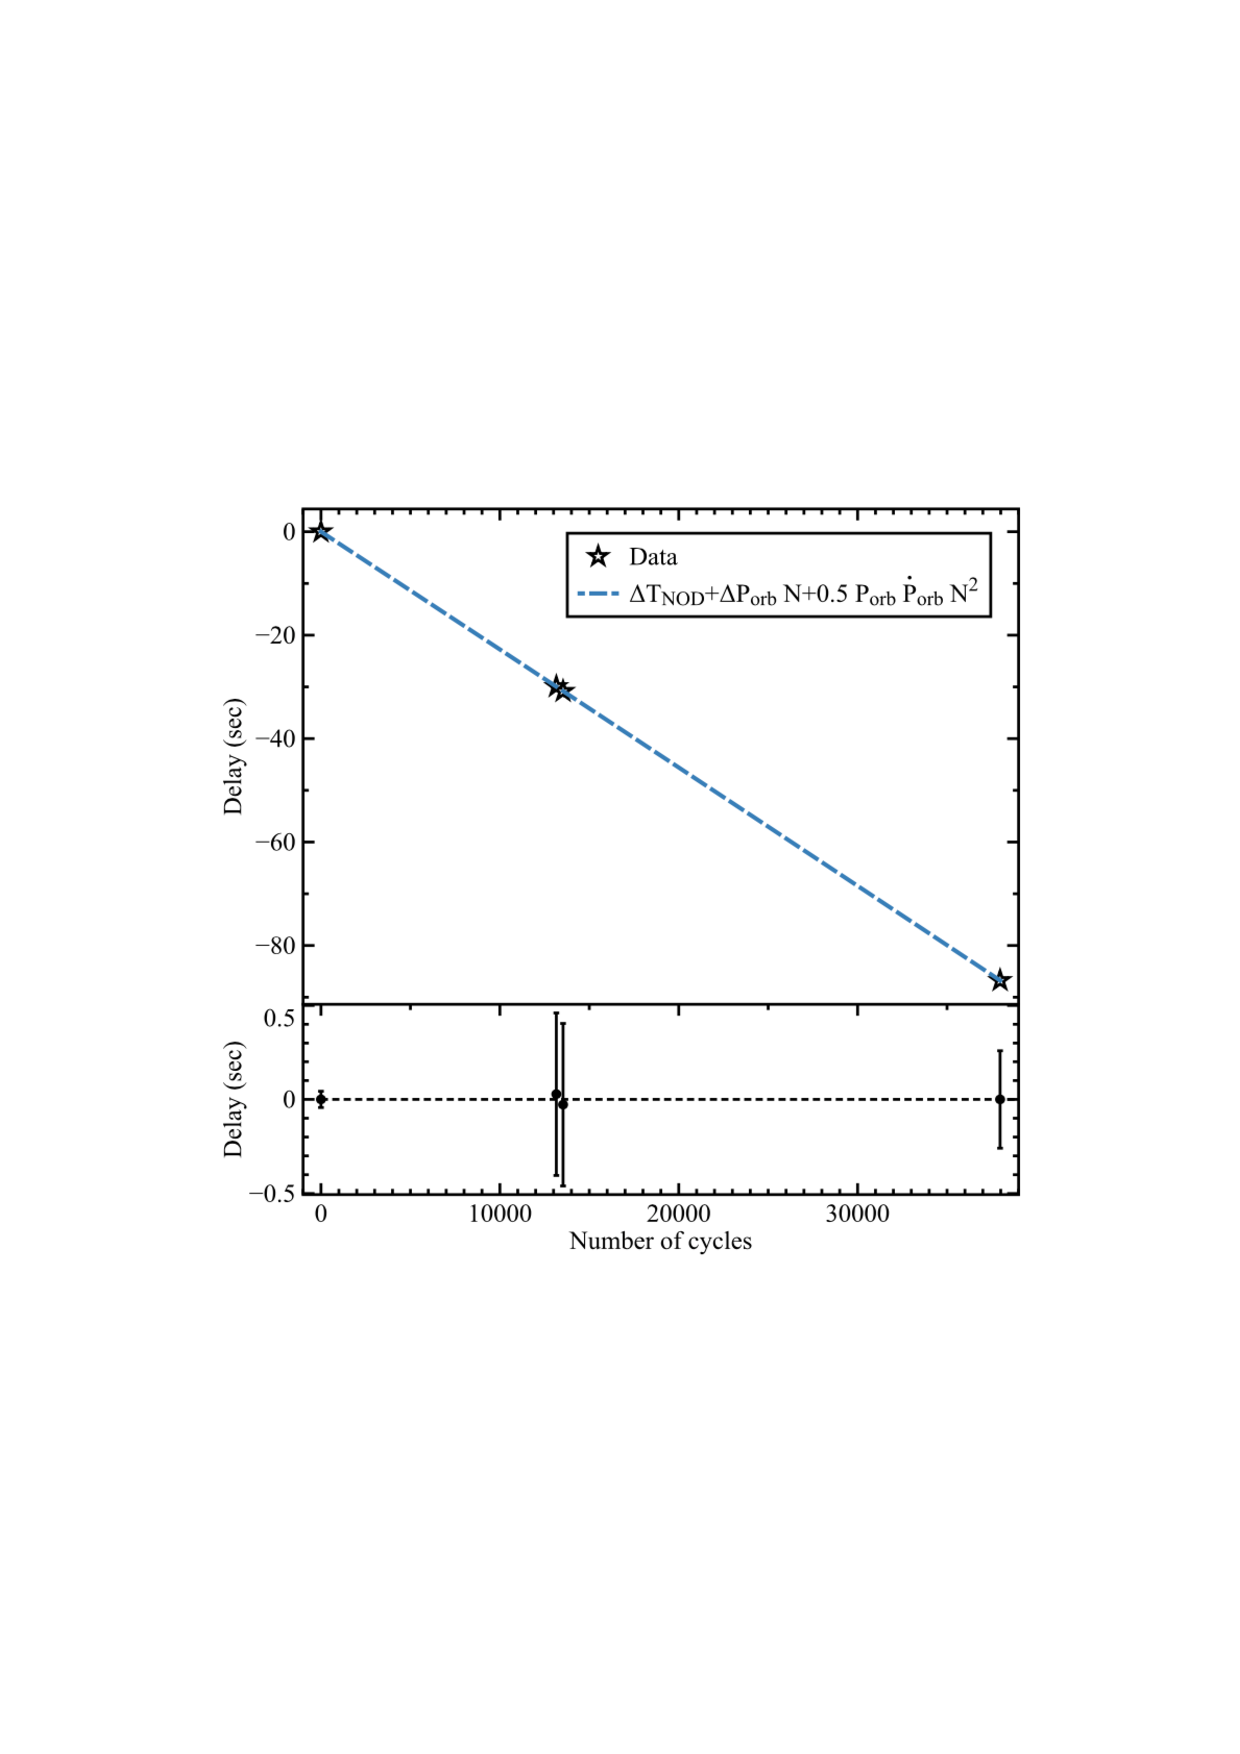
\includegraphics[width=1.1\linewidth]{REVIEW_AMXP/00291_orb_2}
  \label{fig:sfig2}
\end{subfigure}
\caption{\textit{Left Panel:} Orbital evolution of the AMXP \saxj{}. The dashed, dashed-dot and solid curves represent the parabolic trends fit between 1998-2008, 2008-2019, and 1998-2019 subsets of the data, respectively. Residuals relative to the 1998-2008 and 1998-2019 parabolic models are shown in the middle and bottom panels, respectively. The dashed line shown in the bottom panel represents a sinusoid with a 18.2 yr period and 7 s amplitude that has been inserted to tentatively describe the residuals (see \cite{Bult2019c} for more details). The solid line indicates the spin evolution best fit model. \textit{Right Panel:} Orbital evolution of the AMXP IGR J00291+5934. The cyan dashed line represents the best-fitting parabola used to model the data. Residuals in seconds of the time delays with respect to the best-fitting timing solution are shown in the bottom panel. [Figures from \cite{Bult2019c,Sanna2017d}]}
\label{fig:orb_evo}
\end{figure}




\textbf{As shown in the right panel of Fig.~\ref{fig:orb_evo},} a very different evolution is found for IGR J0029+5934, which has orbital parameters very similar to those of \saxj{}, and it is considered its orbital twin. IGR J0029+5934 has shown only four outburst since its discovery, but tight upper limits could be derived on its orbital period derivative, $|\dot P_{orb}| < 5 \times 10^{-13}$ s s$^{-1}$ (90\% confidence level \cite{Patruno2017,Sanna2017d}). This implies a much slower orbital evolution, on a timescale longer than $\sim 0.5$ Gyr, as compared to the fast (up to 2015) orbital evolution of \saxj{}, $\sim 70$ Myr. Although the orbital evolution observed in IGR J0029+5934 is obtained using only four points with large error bars, and more measurements are needed to confirm this result, it seems to be compatible with the expected timescale of mass transfer driven by angular momentum loss via GR, with no need of A\&S mechanism or non-conservative mass transfer. 

\begin{table}
\caption{Accreting Millisecond X-ray Pulsars: secular spin and orbital evolution}
\scriptsize
\begin{center}
\begin{tabular}{lcccccl}
\hline
\hline
Source & \# outbursts & $P_{\rm orb}$ & $T_{ASC}$  & $\dot{P}_{\rm orb}$ & $\dot{\nu}$ & Ref.\\
 &  & (s) & (MJD) & (s/s) & (Hz/s) &\\
\hline
\textbf{AMXP} & & & & & & \\
\hline
NGC 6440 X-2 & 4 & 3457.8929(7) & 55318.04809(2) &  $(-8\div8)\times 10^{-11}$ &$(-5\div5)\times 10^{-13}$ & \cite{Bult2015c}\\
SAX J1748.9--2021 & 4 & 31554.868(3) & 52191.52737(3) &  $3.9(1.1)\times 10^{-11}$ & --& \cite{Sanna2020}\\
IGR J00291+5934  & 4 & 8844.07673(3) &53345.16192640(5)  & $-0.7(2.2)\times 10^{-13}$ & $(-6\div6)\times 10^{-15} $  &  \cite{Patruno2017,Sanna2017d}\\
IGR J17379--3747  & 3 & 6765.84521(3) & 53056.03926(12) &  $−2.5(2.3)\times 10^{-12}$ & --  & \cite{Sanna2018b}\\
SAX J1808.4--3658 & 8 & 7249.1541(2) & 50914.79449(4) & $1.7(0.6)\times 10^{-12}$ & $-1.01(7)\times 10^{-15}$ & \cite{Bult2019c,Sanna2020b}\\
Swift J1756.9--2508 &3  & 3282.3519(5) &  54265.28087(10) &  $1.5(2.8)\times 10^{-12}$ & $-4.8(6)\times 10^{-16}$ & \cite{Sanna2018d,Bult2018b}\\
IGR J17511--3057 & 2 & 12487.50(7) & 57107.85882(8) & $4.4(7)\times10^{-11}$  & -- &  \cite{Riggio2020} \\
IGR J1751--305 & 2 & -- & -- & $(-1.4\div1.4)\times10^{-11}$  & $-5.5(1.2)\times 10^{-15}$ &  \cite{Riggio2011b}\\
\hline
\hline
\end{tabular}\\
\end{center}
$P_{\rm orb}$ is the orbital period, $T_{ASC}$ is the time of passage from the Ascending Node and the reference of the orbital solution, $\dot{P}_{\rm orb}$ is the orbital period derivative.
\label{Tab2}
\end{table}

%%%%%%%%%%%%%%%%%%%%%%%%%%%%%%%%%%%%%%%%%%%%%%%%%%%%%%%%%%%%%%%%%%%%%%%%%%%%%%%%%%%%%%%%%%%%%%%%%%%%%%%%%%%%%%%%%%%%
What causes such an enormous difference between the orbital evolution of two sources with very similar orbital parameters?  
\cite{Tailo2018} have studied the effects of irradiation of the companion star in order to reproduce the evolution of \saxj{}. They have simulated the binary evolution of its possible progenitor system, starting at an orbital period of $\sim 6.6$ h and taking into account angular momentum losses via MB and GR. They also consider the effects of illumination of the donor by both the X-ray emission during accretion phases and the spin-down luminosity of the pulsar. They show that pulsar irradiation is a necessary ingredient to reach the correct orbital period when the donor mass is reduced to the actual value of $0.04-0.06\, M_\odot$. Also it is shown that irradiation alters the internal structure of the donor, causing the companion star to be not completely convective at the values of mass observed for the system and keeping the MB active along the whole evolution (see also \cite{Chen2017}). Mass transfer proceeds through cycles: the donor reacts to the irradiation expanding and starting a phase of large mass-transfer; consequently, mass loss dominates the period evolution. When the thermal relaxation of the envelope takes over, the star radius shrinks and the system detaches (see also \cite{Benvenuto2017} and references therein). In this framework, \saxj{} and IGR J0029+5934 may be at different phases of this cycling behavior, with the first in a phase of high mass transfer rate (and a fast orbital evolution) and the latter in an almost detached phase (with a low mass transfer rate and slow orbital evolution). In both cases, a non-conservative mass transfer is implied with matter expelled from the system by the radiation pressure of the pulsar, that should be stronger in the case of IGR J0029+5934 because of its faster rotation. More details on the orbital evolution of these systems form a theoretical point of view can be found in Chapter 9 of this book. 
%%%%%%%%%%%%%%%%%%%%%%%%%%%%%%%%%%%%%%%%%%%%%%%%%%%%%%%%%%%%%%%%%%%%%%%%%%%%%%%%%%%%%%%%%%%%%%%%%%%%%%%%%%%%%%%%%%%%

In order to test this or other models for the orbital evolution in these systems it is important to continue monitoring the behavior of these and other sources. Other AMXPs have shown more than one outburst for which an orbital solution has been obtained. Long-term evolution of the time of passage from the ascending node of SAX J1748.9--2021 has been clearly observed after combining the orbital solutions of the five observed outbursts to date (in 2001, 2005, 2010, 2015 and 2018). Although marginally significant ($\sim 3.5 \sigma$ confidence level), an orbital period derivative of $\dot{P}_{\rm orb}=3.9(1.1)\times 10^{-11}$ s/s has been determined \cite{Sanna2020}, suggesting again a fast orbital expansion of the system. In the case of IGR J17379--3747, the combination of the ephemerides obtained for the observed outbursts allows to set an upper limit on the orbital period derivative of $-4.4\times10^{-12} < \dot{P}_{\rm orb} < 9.4\times 10^{-12}$ \cite{Sanna2018b}. Swift J1756.9--2508 has been detected in outburst three times (2007, 2009 and 2018) since its discovery; the orbital timing of the source sets an upper limit on the orbital period derivative of $-4.1 \times 10^{-12} < \dot{P}_{\rm orb} < 7.1 \times 10^{-12}$ \cite{Sanna2019}. \cite{Riggio2020} analysed a \nustar{} observation of the 2015 outburst of IGR J17511--3057, obtaining a new local orbital solution. Combining that with the the orbital solution of the 2011 outburst \cite{Riggio2011}, they inferred an orbital period derivative of $\dot{P}_b = 4.4(7) \times 10{-11}$ s s$^{-1}$, suggesting a fast orbital expansion of the binary system similar to that reported for SAX J1748.9--2021. These results are summarised in Table \ref{Tab2}.

\subsection{Not conservative mass transfer?}

Despite the reduced statistics, the majority of the results suggests that these sources are undergoing a fast orbital expansion, notwithstanding the low averaged mass accretion rate observed from these sources.

Besides AMXPs, one of the most evident example of non-conservative mass transfer is given by the slowly rotating (spin period of $\sim 0.59$ s, \cite{Jonker2001}) X-ray pulsar and eclipsing LMXB 4U 1822-37, which shows a persistent X-ray luminosity of $\sim 10^{36}$ erg/s and an orbital period of $\sim 5.57$ h, measured from the periodic eclipse of the X-ray source and confirmed through the timing of the X-ray pulsations. The compilation of the eclipse times over the last 40 years shows a fast orbital expansion at a rate of $\dot P_{orb} \sim 1.5 \times 10^{-10}\, M_\odot/yr$ (see e.g. \cite{Chou2016,Mazzola2019}). The delays on the eclipse arrival times with respect to a constant orbital period show a clear parabolic trend, which implies a constant orbital period derivative, more than three orders of magnitude what is expected from conservative mass transfer driven by MB and GR (e.g. \cite{Burderi2010,Iaria2011}). Mechanisms based on the gravitational quadrupole coupling of the companion star with the orbit (see e.g. \cite{Applegate1992,Applegate1994}) have been investigated, however, they resulted not suitable since the ($\sim 0.3\, M_\odot$) companion star lacks internal power to produce such a large orbital period variation (e.g. \cite{Mazzola2019}). 
%
A possible explanation is given by a highly not conservative mass transfer, in which the companion star transfers mass at a high rate. Most of the transferred mass is then expelled from the system by the strong radiation pressure of the central source emitting at the Eddington limit. In fact, it has been proposed that 4U 1822-37 is accreting at the Eddington limit (while just 1\% of the total X-ray luminosity is visible due to the high inclination angle, $80-85^\circ$, \cite{Iaria2011}), while the companion star is transferring at a higher rate (of the order of seven times Eddington, \cite{Burderi2010}), and most of the transferred mass is expelled from the system by the radiation pressure producing strong outflows and winds. 

Indeed, there are other indirect evidences of a non-conservative mass transfer in AMXPs. \cite{Marino2019} have analysed a sample of AMXPs, starting from XTE J0929-314 \cite{Marino2017}, finding that the averaged (over the time since their discovery) X-ray luminosity of most sources of the sample is significantly lower than what would be predicted by conservative mass transfer driven by GR and/or MB. Comparing their averaged X-ray luminosity with that predicted for a conservative mass transfer, a lower limt on the source distance may be estimated. Based on a sample of 18 sources, strong evidence of a non-conservative mass transfer was found for five sources, for which the estimated distance lower limits are significantly higher than their known distances, while hints of mass outflows are found in further six sources of the sample. The discrepancy can be fixed under the hypothesis of a non-conservative mass transfer in which a fraction of the mass transferred onto the compact object is swept away from the system, likely due to the radiation pressure of the rotating magnetic dipole and/or pulsar wind.

A similar argument has also been proposed for the black-hole X-ray Binary and microquasar V404 Cyg  \cite{Ziolkowski2018}; considering the donor evolution and mass transfer in the microquasar V404 Cyg and X-ray observations of its two outbursts, the authors find that the average mass accretion rate is substantially lower than the model mass-loss rate from the low-mass giant donor; to fix this discrepancy, they propose that a large fraction of the mass flowing from the donor leaves the binary in the form of outflows from the accretion disc around the accretor.   
%
We can conclude that, regardless of the nature of the accretor and the radiation emitted, it seems that radiation pressure has an important role in limiting the accretion of matter onto the compact object and in initiating a not-conservative mass transfer in LMXB systems, which may be a common feature in these systems, possibly related (as a cause or consequence) to the transient behavior itself. 


\section{Summary and Open questions}
%\textbf{1) Spin frequency max < 600 Hz; 2) Why only 20\% LMXB shows pulsations?; 3) Pulsations in UV and Optical: origin }
Despite the amount of information we have gained in the last two decades of observations and theoretical studies of AMXPs, several issue still remain to be addressed, as for instance the torque imparted by the accreting matter onto the NS, probably hidden in most cases from the strong timing noise present in the timing of the spin period. Is the spin-up or spin-down of the NS overwhelmed with the large timing noise? Moreover, what is the origin of this large timing noise? Movements of the hot spot on the NS surface caused by flux variations have been proposed to explain the large timing noise, although it is not clear why in some sources (e.g. \saxj{}) is appears to be much stronger than in other sources (e.g. \ IGR J00291+5934). Even more puzzling are the orbital residuals observed in \saxj{} and the different behaviour observed in IGR J00291+5934, as well as the role of non-conservative mass transfer in AMXPs and LMXBs in general. Beside that, there are other important issues that should be addressed and are briefly described in the following. 

The discovery of AMXPs and the subsequent discovery of transitional millisecond pulsars (see Chapter 7 of this book for further details) has confirmed the recycling scenario. As a consequence of that, we improved our understanding of the formation of millisecond pulsars, which are accelerated by the accretion of matter and angular momentum during the LMXB phase, and of the evolutionary path linking the progenitors, i.e. LMXBs, to the end products of the evolution, i.e. Black-Widow pulsars and Redbacks, possibly through the transitional phase. Nevertheless, several open questions remain to be addressed, the first one regarding pulsations themselves.  
In fact, apart from the presence of coherent pulsations, AMXPs resemble the behaviour of transient LMXBs of the atoll class. Both the spectral properties and the aperiodic and quasi-periodic variability (so-called QPOs) are very similar between AMXPs and not-pulsating LMXBs (see e.g.\ \cite{Wijnands1999}, see also \cite{Patruno2012} for a review). Similar to LMXBs, AMXPs show type-I X-ray bursts and all the associated phenomenology, as for example the presence of (quasi-coherent) oscillations at the spin frequency of the NS during type-I X-ray bursts. From the observation of burst oscillations we know that many NS in LMXBs indeed rotate at millisecond periods. However, despite all these similarities, the large majority of LMXBs harbouring a NS do not show coherent pulsations, not even when the mass accretion rate decreases (for instance in transient systems) enough to allow the magnetosphere to expand outside the NS surface. The observation of an intermittent behaviour of coherent pulsations in some AMXPs (see e.g. the case of Aql X-1 or HETE J1900.1-2455) has suggested that magnetic field burial caused by accretion of fresh matter may play a role (see e.g. \cite{Cumming2001} and references therein). However, it is not clear whether this can explain the lack of pulsations in most of LMXBs or other factors contribute in hampering the detection of pulsations in these sources. These may be for instance a smearing of the pulsations by an optically thick corona, a smearing of pulsations due to gravitational light bending, alignment of the NS magnetic and rotational axes, onset of MHD instabilities at the disk/magnetospheric boundary. None of these models, however, furnish a satisfactorily explanation valid for all the cases (see a discussion in \cite{Patruno2012,Campana2018}).

Even more puzzling is the lack of radio pulsations in both AMXPs and LMXBs during X-ray quiescence. In principle, when the accretion of matter stops during (long) quiescent periods, the mechanism producing radio (or gamma-ray) pulsations should resume and the millisecond pulsar should shine in radio (or gamma-ray) as a rotation-powered pulsar. However, this has been observed to date in just one source, the AMXP and transitional pulsar IGR J18245-2452 (J18245 hereafter) in the Globular Cluster M28 \cite{Papitto2013b}. This source has been first observed as a radio millisecond pulsar (spinning at 3.93 ms) in a binary system with a 11-h orbital period. In 2013 it went into X-ray outburst and was discovered as an AMXP; soon after the end of the outburst J18245 was detected again as a radio pulsar, demonstrating that the transition between the rotation-powered and the accretion-powered regime can occur on short timescales (in about 10 days or even less). It is worth noting that the other 2-3 sources, belonging to the transitional millisecond pulsar class, also show radio pulsations during X-ray quiescence and X-ray pulsations during the so-called disk state with (possibly) a low-level of accretion. However, none of these sources ever showed an X-ray outburst to date similar to the one showed by J18245 or the other AMXPs. The compelling possibility that these systems could swiftly switch from accretion-powered to rotation-powered magneto-dipole emitters during quiescence gives the opportunity to study a phase that could shed new light on the not yet cleared up radio pulsar emission mechanism. Therefore, if the swing between the rotation-powered and the accretion-powered pulsar can happen on fast timescales, why is this  observed just in few cases? Why radio millisecond pulsations at the known spin period have never been detected in other LMXBs or AMXPs during X-ray quiescence? 

In the framework of the so-called radio-ejection model \cite{Burderi2001}, the radio pulsar mechanism switches on when a significant reduction of the mass-transfer rate occurs. The accretion of matter onto the NS is then inhibited by the radiation pressure from the radio pulsar, which may be capable of ejecting out of the system most of the matter overflowing from the companion-star Roche lobe. One of the strongest predictions of this model is the presence, during the radio-ejection phase, of a strong wind of matter emanating from the system. The non-detection of radio pulsations in this situation may be due to free-free absorption of the radio signal interacting with the ejected matter. A possibility to test this scenario is, therefore, to performed deep (tens of hours) radio observations of these sources at high radio frequency (above $5-6$ GHz), since the cross-section of free-free absorption decreases with frequency as $\nu^{-2}$ (see e.g. \cite{Iacolina2009,Iacolina2010}). However, the question remains: why do transitional millisecond pulsars, and J18245 in particular, behave in a different way, showing radio pulsations when the X-ray emission is off? Perhaps, a favourable geometry, e.g. a relatively low inclination angle of the system, may reduce the amount of matter along our line of sight, since most of the matter is expected to lie in the equatorial plane, and therefore reduce the amount of free-free absorption in these systems. Alternatively, pulsating radio emission should be searched in systems with long orbital periods, in which the matter transferred by the companion star is spread over a wider orbit. 

Despite the fact that radio pulsations remain elusive in AMXPs, sporadic detection of transient emission in the radio band has been reported in a few cases. On the other extreme of the electromagnetic spectrum, in the gamma-ray band, searches of AMXPs counterpart is also quite difficult. Because of the paucity of photons at such high energies, in order to obtain a statistically significant detection, it is necessary to integrate over several years. The analysis of $\sim 6$ yr of data from the Large Area Telescope on board the Fermi gamma-ray Space Telescope (Fermi-LAT) revealed a possible gamma-ray counterpart of \saxj{}, at a significance of $\sim 6 \sigma$, with a position compatible with that of the source within the $95\%$ confidence level \cite{deOnaWilhelmi2016}. However, the search for coherent pulsations did not produce a significant detection taking into account the number of trials. Uncertainties in the source position, orbital motion of the pulsar as well as the intrinsic evolution of the pulsar spin, which still are not known with enough precision to maintain the phase over years, are likely the causes of the non detection. A precise knowledge of the spin and orbital parameters of AMXPs are of fundamental importance to allow deep searches of their counterparts in the gamma-ray band, which has the advantage of not suffering the free-free absorption as in the radio band, but the disadvantage of the reduced number of photons, which requires folding over years in order to reach the statistics needed for detecting a (weak) pulsed signal. 

On other other hand, searches of the optical counterpart of these systems has given interesting, unexpected results. In several AMXPs, the optical counterpart during X-ray quiescence appears surprisingly luminous, inconsistent with both intrinsic emission from the companion star and X-ray reprocessing (e.g. \cite{Homer2001,DAvanzo2009,DAvanzo2011}). In fact, the optical counterpart shows an approximately sinusoidal modulation with photometric minimum at the superior conjunction of the pulsar. The lack of ellipsoidal, double-humped variations, rules out an origin from intrinsic emission from the companion star, while it is best explained as caused by the irradiated surface of the companion star. Given the lack of significant X-ray emission during quiescence, this has been interpreted as a strong (indirect) evidence that a rotating magneto-dipole powers the quiescent emission of AMXPs \cite{Burderi2003,Campana2004}. In fact, the magnetic dipole rotator, if active during quiescence, has a bolometric luminosity given by the Larmor's formula and may power the reprocessed optical emission. 

Even more puzzling is the recent discovery of optical pulsations at the NS spin period in one of the transitional pulsars, PSR J1023+0038 \cite{Ambrosino2017,Papitto2019}, the first time ever from a millisecond pulsar. Optical pulsations, with a maximum pulsed optical luminosity of $L_{pulse} \simeq 0.01 L{opt} \simeq 10^{31}$ erg s$^{-1}$, were observed when the source was in a bright active state corresponding to an X-ray luminosity of $7\times 10^{33}$ erg s$^{-1}$ (see Chapter 7 of this book). More recently, optical and UV coherent pulsations were observed in the AMXP \saxj{} \cite{Ambrosino2020}, with a similar optical luminosity and pulsed fraction as observed in PSR J1023+0038. Optical pulsations in \saxj{} were observed during the rising phase of the 2019 outburst (at an X-ray luminosity of a several $10^{34}$ erg s$^{-1}$), and during the decay of the outburst at a similar X-ray luminosity level. Several options are being considered in order to explain the large optical pulsed luminosity, while a clear explanation still remains elusive. Certainly, future optical observations with a fast photometer during X-ray quiescence or at the peak of an X-ray outburst, possibly performed simultaneously to high-time resolution X-ray observations, will give further information able to discriminate among different possibilities.

%*** Minimum period of NS
From the discussion above it is clear that, despite the amount of observations and information obtained on AMXPs to date, there are still several issues that deserve further investigation, also considering that some new discoveries have raised other new questions. Nevertheless, one of the most important open questions about AMXPs is their spin period distribution and, most of all, the minimum spin period for a NS. Since (recycled) millisecond pulsars are accelerated during the LMXB phase, we expect that the minimum period of a NS is reached during this accretion phase, before the starting of the (non-accreting) spin-down phase caused by the emission of the magnetic dipole rotator. Hence, we expect that the fastest spinning NS should reside in an AMXP. Since the maximum frequency of a NS depends on its compactness, that is on its mass to radius ratio, the detection of the maximum spin frequency of NS may give strong and important constraints on the EoS of ultra-dense matter.
However the distribution of spin frequencies of the ensemble of AMXPs has an abrupt cutoff at about 730 Hz (e.g. \cite{Patruno2017b}), well below the maximum spin frequency allowed by the majority of realistic EoS. We are left therefore with the following questions: is the maximum frequency of NS telling us something related to the EoS of ultra-dense matter? Alternatively, which is the factor limiting the spin of NS well below the maximum possible possible frequency? Several possibilities have been proposed as a limiting factor for the NS rotation, such as emission of Gravitational Radiation \cite{Hartman2011,Papitto2011b}, the presence of a (not completely decayed) magnetic field \cite{ Patruno2012}, bias caused by a fast orbital motion \cite{Burderi2001}, and so on. However, none of these possibilities seems to explain all the phenomenology of AMXPs and LMXBs, and further investigation is needed to assess this fascinating question. To this aim, future X-ray missions, with large effective area and fast timing capabilities, possibly coupled with polarimetric capabilities (as is the case of the enhanced X-ray Timing and Polarimetry mission, eXTP) may be fundamental to put forward the research in this field and to open an new era of exciting discoveries on millisecond pulsars.    


\begin{comment}

\section{Observational overview of individual AMXPs}

\subsection{SAX J1808.4-3658}

The most regular among recurrent AMXPs, and therefore the best studied of these sources, \saxj is the first discovered AMXP, which has shown an X-ray outburst every $1.6-3.5$ years, the latest one occurred in 2019 \cite{Bult2019c}. The outburst light curve is characterised by a fast rise (on a couple of days timescale), a slow exponential decay (with a timescale of $\sim 10$ days) followed by a fast decay (with a timescale of $\sim 2$ days). After the end of the main outburst, usually a flaring activity, called reflares, is observed, with a quasi-oscillatory behaviour and a variation in luminosity of up to three orders of magnitude on timescales of $\sim 1-2$ days \cite{Patruno2016}. Moreover a strong $\sim 1$ Hz oscillation is observed to modulate the reflares \cite{Bult2014}. A similar behaviour was also observed in the AMXP NGC 6440 X-2 \cite{Patruno2013}. The reflaring behaviour has no clear explanation, however, \cite{Patruno2016} proposed a possible explanation in terms of either a strong propeller with a large amount of matter being expelled from the system or a trapped (dead) disk truncated at the co-rotation radius \cite{DAngelo2012}.
Several thermonuclear X-ray bursts have observed during the source outbursts, some of which exhibited characteristics compatible with photospheric radius expansion X-ray bursts likely originating in a flash of pure helium layer created by stable burning hydrogen \cite{Galloway2006,Galloway2008}. Combining X-ray burst from different outbursts, \cite{Galloway2006} estimated a source distance of $3.5\pm0.1$ kpc.

Coherent timing analyses of the X-ray pulsations revealed a 2.01hr orbital period \cite{Chakrabarty1998}. Moreover, it showed that, with few exceptions (see e.g. \cite{Burderi2006}), no clear accretion-induced spin frequency variations are detectable during the X-ray outbursts \cite{Hartman2008,Patruno2012a,Patruno2017}. However, combining the analysis of multiple outbursts it appears clear a secular evolution of the spin frequency compatible with a constant spin-down derivative of magnitude $\sim10^{−15}$ Hz s$^−1$ \cite{Hartman2008,Patruno2012,Sanna2017c,Bult2019c}, likely reflecting a magnetic dipole torque acting during quiescence. Long-term variation of the binary period indicates a fast expansion of the orbit, which has been explained with either a highly non-conservative mass-transfer \cite{DiSalvo2008,Burderi2009, Sanna2017c}, or, alternatively, a gravitational quadrupole coupling mechanism acting between the system and the companion star \cite{Hartman2008,Patruno2012,Sanna2017c}.

The pulsar mass function $f(m_2,m_1,i)\sim 3.8\times 10^{-5}$ M$_\odot$ gives a minimum companion mass of $m_2=4.4\times10^{-2}$ M$_\odot$ for a NS mass $m_1=1.4$ M$_\odot$. Statistical considerations on the a priori probability distribution of the binary inclination angle suggests a $m_2\leq$ 0.14 M$_\odot$, likely, Brown Dwarf companion star \cite{Bildsten2001,Deloye2008,DiSalvo2008}.

V4584 Sagittarii, the optical/IR counterpart of \saxj{}, was discovered during the 1998 outburst with magnitude $V=16.6\pm0.2$, $R=16.1\pm0.2$, $I=15.6\pm0.2$, $J=15.0\pm0,1$, $H=14.4\pm0.1$, $K=13.8\pm0.1$. Optical flux consistent with an X-
ray heated accretion disk and an inclination of $i=51\pm18$ degrees (90\% c.l.)\cite{Wang2001}. Radio observations performed with ATCA revealed a transient radio counterpart (flux $\sim$0.8 mJy) interpreted as synchrotron emission, which could be consistent with the IR transient excess. This suggests the presence of relativistic jets and/or outflows ejected from the binary. 
Optical and UV observations of the source performed with high-temporal resolution instruments allowed to detect, for the first time, coherent oscillations at the NS spin frequency (Ambrosino et al. in prep).


\subsection{XTE J0929-314}

XTE J0929-314 is a high-latitude X-ray source discovered by the All-Sky Monitor aboard \rxte{} in 2002 and observed in outburst for about 53 days starting from May 2 \cite{Galloway2002a}. Analysis of the high time resolution \rxte{} data allowed to detect persistent $\sim185$ Hz pulsations \cite{Remillard2002}. Doppler modulation of the coherent X-ray pulsation is compatible with an ultra-compact nature of the binary with an orbital period of $\sim48$ minutes \cite{Galloway2002}. Moreover, the pulsar showed a clear spin down at an average rate of $\dot{\nu}\sim-9\times 10^{-14}$ Hz s$^{-1}$ for which the following possible mechanisms have been isolated: a) magnetic coupling to the accretion disk; b) magneto-hydrodynamic wind; c) gravitational radiation from the rapidly spinning pulsar (see \cite{Galloway2002} and references therein). No radio pulsation has been detected during the quiescence state of the source with an upper limits of 68 $\mu$Jy at 6.4 GHz and 26 $\mu$Jy at 8.5 GHz \cite{Iacolina2009}.

Spectral properties have been investigated modelling the broad-band energy spectrum collected combining \chandra{} and \rxte{} observations during the 2002 outburst of the source. The spectrum is well modelled by an absorbed Comptonization ($\Gamma\sim1.7$) plus blackbody ($kT\sim 0.7$ keV) model. No emission or absorption features are found in the \chandra{} high-resolution spectrum \cite{Juett2003}.


The pulsar mass function $f(m_2,m_1,i)\sim 2.7\times 10^{-7}$ M$_\odot$ gives a minimum companion mass of $m_2=8\times10^{-3}$ M$_\odot$ for a NS mass $m_1=1.4$ M$_\odot$. Considerations on the binary parameters suggested a $m_2\simeq$ 0.1 M$_\odot$ White Dwarf companion star and a moderately high inclination. Multiwavelength study of XTE J0929-314 have been performed allowing to detect V variable optical \cite{Greenhill2002,Cacella2002} and radio \cite{Rupen2002} counterparts compatible with the X-ray source position measured with the \chandra{} X-Ray Observatory \cite{Juett2003}. C \rom{3}/N \rom{3} and $H\alpha$ emission lines were reported in the optical spectrum \cite{Castro2002}, while a radio counterpart (during the outburst) was detected with the VLA at 4.86 GHz \cite{Rupen2002}.

\subsection{XTE J1751-305}

The NS X-ray binary XTE J1751-305 was detected for the first time by \rxte{} on April 3, 2002 \cite{Markwardt2002a}. During the outburst coherent X-ray pulsations at $\sim$435 Hz were observed and a full orbital solution has been determined revealing a $\sim42$ minute orbital period and the ultra-compact nature of the binary system \cite{Markwardt2002}. Phase-coherent timing analysis of the 10-days long outburst allowed to constrain a spin up effect with an average rate of $(3.7\pm1.0)\times10^{-13}$ Hz s$^{-1}$ \cite{Papitto2008}. \inte{} detected a possible new outburst of the source on March 28, 2005 \cite{Grebenev2005}. The short duration ($\sim2$ days) and the weak intensity of the outburst (peak flux almost ten times dimmer than the first outburst) combined with the lack of high resolution timing data did not allow to make a clear association with XTE J1751-305 \cite{Swank2005}. Very similarly, on April 5, 2007, \rxte{} observed only for a short time the source that resulted too dim to detect pulsations. However, a clear identification of the source has been possible thanks to a follow-up \swift{} observation \cite{Markwardt2007}. A fourth outburst was first observed with \inte{} \cite{Chenevez2009}, and shortly after followed by \rxte{} (casually observing the newly discovered AMXP IGR J17511-3057 \cite{Markwardt2009}). X-ray pulsations were clearly detected and combined to estimate an updated orbital solution \cite{Riggio2011}. 

Spectral analysis of the 2002 outburst revealed that the broad-band X-ray spectrum of XTE J1751-305 requires three components: two soft components modelling the thermal emission from the accretion disk ($kT\sim0.6$ keV) and the accretion spot ($1$ keV) on the NS surface, and a hard component representing the thermal Comptonization in a plasma with $kT_e\sim40$ keV and optical depth $\sim1.5$ in a slab geometry \cite{Gierlinski2005}. No clear evidence for narrow or broad emission or absorption lines has been detected in the time-averaged spectrum. Upper limits of 4 and 6 eV have been estimated for the strength of narrow (FWHM$\sim0.1$ keV) and broad (FHWM$\sim0.7$ keV) Fe $K\alpha$ emission lines \cite{Miller2003}. 

The NS mass function $f(m_2,m_1,i) = 1.3\times10^{−6}$ M$_\odot$ allows to infer a minimum companion mass of $m_2>1.4\times10^{-2}$ M$_\odot$ for an inclination angle of $i<75^\circ$ (lack of eclipses or dips) and a NS mass $m_2=1.4$ M$_\odot$, suggesting a heated He or C/O white dwarf companion \cite{Deloye2003}.
Studies of optical and near-infrared images of the region around XTE J1751-305 revealed no stars within the \chandra{} positional error circle (0''.7; \cite{Markwardt2002}). Upper limits for the counterpart $R>23.1$, $I>21.6$, $Z>20.6$, $J>19.6$, $K>19.2$ have been estimated \cite{Jonker2003}. No evidence for GW emission from XTE J1751-305 has been found in the frequency bands 434.5-436.5 Hz, 620.5-622.5 Hz, or 869.5-871.5 Hz. No candidate templates passed both threshold and coincidence requirements between LIGO Hanford and LIGO Livingston observatories \cite{Meadors2017}. 

\subsection{XTE J1814-338}      

The accreting millisecond X-ray pulsar XTE J1814-338 was discovered on June 5 2003 during the scanning of the Galactic-center region performed by \rxte{}. Standard timing analysis showed the presence of a pulsed signal at the frequency of $\sim314$ Hz interpreted as the spin frequency of a NS harboured in a binary system with a 4.3 hrs orbital period \cite{Markwardt2003}. A peculiar negative spin frequency derivative (spin-down) of $\dot{\nu}\sim -7\times 10^{-14}$ Hz has been reported combining the observations covering the almost 50-days long outburst \cite{Papitto2007}.   
Numerous Type I X-ray bursts (28 in total) have been observed from XTE J1814-338 during its outburst. Burst oscillations with frequency in the vicinity of the 314 Hz pulsar frequency have been reported for all the detected Type I X-ray bursts  (see e.g. \cite{Strohmayer2003,Watts2005}).  A source distance of $8\pm1.6$ kpc was inferred from one of the Type-I burst showing signs of photospheric radius expansion \cite{Strohmayer2003}.

An optical counterpart of XTE J1814-338 at $R\sim18.3$ has been observed during the outburst; moreover, hydrogen and helium emission lines were detected through optical spectroscopy, suggesting for a non-degenerate companion \cite{Krauss2005}. 
Optical observations in quiescence reported a rather faint ($R\sim22.5$ and $V\sim23.3$; \cite{DAvanzo2009}) counterpart.
A multiband Very Large Telescope (VLT) campaign carried in 2009 (during quiescence) shows an irradiated companion star that requires an energy source compatible with the spin-down luminosity of a millisecond pulsar \cite{Baglio2013}. This proves further evidence that AMXPs might turn on as radio pulsars when in quiescence. Doppler tomography of the Bowen region applied to the 2003 outburst allowed to constrained the binary mass ratio  $q\sim0.123$, the inclination angle $35^\circ<i<78^\circ$ and the companion mass $0.19$ M$_\odot$ $<m_2<0.32$ M$_\odot$ assuming a NS mass ranging between M$_\odot$ $<m_1<2.7$ M$_\odot$. The dynamical mass constraints confirmed previous suggestions of a significantly bloated main-sequence M-type companion star \cite{Wang2017}.

\subsection{XTE J1807-294}

The transient X-ray binary XTE J1807-294 was first detected in outburst on February 2003 with \rxte{} while performing monitoring observations of the Galactic center region \cite{Markwardt2003}. Coherent pulsations at the frequency of $\sim190$ Hz were detected, suggesting the detection of a new AMXP. Significant sinusoidal modulation of the X-ray pulsations compatible with an orbital period of $\sim40$ minutes and projected semi-major axis of $\sim4.8\times 10^{-3}$ lt-s were established \cite{Markwardt2003b}, making XTE J1807-294 a member of the ultra-compact binary group. Timing analysis of the almost 120-days long outburst (exceptionally long with respect to the average outburst duration shown by AMXPs) allowed to refine the orbital solution and to constrain the NS spin evolution during the accretion phase (see e.g. \cite{Kirsch2004,Riggio2007,Riggio2008,Chou2008,Patruno2010b}). Pulse-shape modelling analysis have been carried out using the \rxte{} observations of the source, allowing to constrain the mass and radius of the NS to $1-2.5$ M$_\odot$ and $\sim12$ km, respectively \cite{Leahy2011}. Simultaneous twin kHz QPOs have observed and investigated in the power spectra of XTE J1807-294 (see e.g. \cite{Linares2005,Zhang2008,Tasheva2018}). 

The 0.5-200 keV broad-band spectral analysis of XTE J1807-294 obtained combining almost simultaneous \inte{}, \rxte{} and \xmm{} observations showed that the source spectrum is well described by a combination of thermal Comptonization (with electron temperature $kT_e\sim40$ keV) and a disk black body (with temperature $kT_B\sim0.8$ keV). Assuming a binary inclination $60^\circ<i<83^\circ$ an inner disk radius lying in the range 20-40 km (for the distance of 8 kpc) has been suggested \cite{Falanga2005a}. Neither absorption nor emission lines have been reported during the outburst (see e.g. \cite{Campana2003}). 

The pulsar mass function $f(m_2,m_1,i) = 1.6\times10^{−7}$ M$_\odot$ allows to infer a minimum companion mass of $m_2>7\times 10^{-3}$ M$_\odot$ for an inclination angle of $i = 90^\circ$ and a NS mass $m_2=1.4$ M$_\odot$, suggesting a very low mass dwarf origin. Binary evolution scenarios applied to ultra-compact X-ray binaries suggest that the donor star could be either a C/O white dwarf or a He white dwarf \cite{Deloye2003}. Constraints on the companion mass ($m_2<0.022$ M$\odot$) obtained from the spectral analysis XTE J1807-294 \cite{Falanga2005a} seems to favours the former scenario. No counterparts have been reported at any wavelength during either outburst or quiescence. A candidate optical counterpart detection within the 0''.6 \chandra{} error circle (90\% confidence level) was reported in 2009 \cite{DAvanzo2009} with $V\sim22.1$ and $R\sim21.4$. No variability has been observed, with upper limits of 0.1 mag.



\subsection{IGR J00291+5934}

IGR J00291+5934 is a transient LMXB observed in outburst for the first by \inte{} on 2004 December 2 \cite{Shaw2005}. Hints for possible outbursts occurring already in 1998 and 2001 have been found from the re-analysis of the \rxte{}/ASM light curve of the source \cite{Remillard2004}. Detection of coherent X-ray pulsations at $\sim599$ Hz (the fastest among the known AMXPs; \cite{Eckert2004,Markwardt2004a}) and Type-I X-ray burst \cite{Kuin2015} revealed the NS nature of the compact object harboured in the binary system. Analysis of the \rxte{} observations of the outburst highlighted sinusoidal variation of the pulsations on timescales of $\sim147$ minutes compatible with orbital Doppler modulation \cite{Markwardt2004b,Galloway2005}. Highly sinusoidal pulse profiles have been observed across a wide range of energies \cite{Galloway2005,Falanga2005b} characterised by soft lags with a complex energy dependence \cite{Galloway2005,Falanga2007}. Coherent timing analysis of the 2004 outburst revealed a spin derivative of $8.5\pm1.1 \time 10^{-13}$ Hz s$^{-1}$ \cite{Falanga2005b,Burderi2007}, compatible with an accretion torque spinning up the NS during outburst \cite{Burderi2007}.  
The source has been detected in outburst again in August and September 2008, showing two separate outbursts with a peak flux level half that observed in 2004 \cite{Chakrabarty2008, Lewis2008}. Finally, on July 2015, a fourth outburst closely resembling the behaviour observed in 2004 has been reported \cite{Sanna2015,DeFalco2017,Sanna2017d}. Timing analysis of the four outbursts allowed to refine the orbital parameters of the system (see e.g. \cite{Patruno2010,Hartman2011,Papitto2011c,Sanna2017d} and to constrain secular evolution of the spin frequency (significant spin-down  of $\dot{\nu}\sim-4\times10^{-15}$ Hz s$^{-1}$; \cite{Patruno2010, Hartman2011, Papitto2011c} and the orbital period (upper limit on the orbital period derivative of $|\odot{P}_{orb}|< 6\times 10^{-13}$ s s$^{-1}$; \cite{Patruno2017,Sanna2017d}. 

Aperiodic timing analysis of IGR J00291+5934 revealed an unusual amount of timing noise at very low frequencies (0.01-0.1 Hz). Interestingly, harmonically related QPOs at $\sim20$ mHz and $\sim40$ mHz \cite{Linares2007,Hartman2011} and a prominent 8 mHz QPO (< 2 keV, \cite{Ferrigno2017}) observed in the 2004-2008 and the 2015 outbursts, respectively, resemble the low-frequency QPOs observed in black holes \cite{Linares2007} rather than the feature typically seen in accreting NS. Coupling between the mHz QPOs and the coherent X-ray pulsation of IGR J00291+5934 has been investigated using the \rxte{} and \xmm{} observations of the source \cite{Bult2017}.

The spectral analysis of the unique Type-I X-ray burst exhibited by IGR J00291+5934 provided indications of a photospheric radius expansion phase allowing to infer a source distance of $d = 4.2\pm0.5$ kpc \cite{Bozzo2015,DeFalco2017}.


Broad-band spectral observations performed during the 2004 and the 2015 outbursts reported the source in a typical hard state dominated at energies by a Comptonization of soft photons (likely produced in the NS surface) by an electron population with kTe $30-50$ keV, and at lower energies by a blackbody component with kT $0.5-1$ keV \cite{Falanga2005b,Sanna2017d}. No signature of the emission from the NS hot spot blackbody has been reported from the study of simultaneous \rxte{}-\chandra{}/HETGS observations collected towards the end of the 2004 outburst \cite{Paizis2005}. The \xmm{}/\nustar{} energy spectrum revealed also the presence of a moderately broad, neutral Fe emission line and four narrow absorption lines as well as a strong correlation between the pulse profile and the blackbody component, suggesting that the latter component resides at the NS surface \cite{Sanna2017d}.

The pulsar mass function $f(m_2,m_1,i)\sim 2.8\times 10^-5$ M$_\odot$ implies a companion mass of $m_2=3.9\times 10^{-2}$ M$_\odot$ for a NS mass of 1.4 M$_\odot$ and inclination angle $i=90^\circ$. Stellar evolution simulations predicted a hydrogen-rich white or brown dwarfs for the secondary star (see \cite{Bildsten2001}). The optical counterpart ($R\sim17.4$) of IGR J00291+5934 has been tentatively identified on 4 December 2004 by the Robotic Palomar 60-inch Telescope \cite{Fox2004} and confirmed by the 4.2-m William Herschel Telescope on La Palma \cite{Roelofs2004} and the Keck I 10-m telescope (Filippenko et al. 2004). IR counterpart of the source has been reported on 8 December 2004 with preliminary magnitudes of $J=16.8\pm0.1$, $H=16.8\pm0.3$, $K=16.1\pm 0.2$ \cite{Steeghs2004}. An optical/NIR photometric study in quiescence performed in 2005 with the 3.6-m Telescopio Nazionale Galileo allowed to determine the VRIJH counterparts of IGR J00291+5934 as well as the observation of optical variability consistent with the orbital period \cite{DAvanzo2007}. The optical counterpart has been observed again on 25 July 2015 with the MASTER-IAC robotic telescope \cite{Rebolo2015b}, detection confirmed by the 2-m Liverpool Telescope \cite{Kopac2015} and the 2-m Faulkes Telescope North at Maui \cite{Russell2015}. Observation of the Radio counterpart of the source at 15 GHz has been reported on 4 December 2004 with the Ryle Telescope in Cambridge \cite{Pooley2004}, not confirmed by a follow up observation with the same observatory (upper limits of $\sim0.6$ mJy; \cite{Fender2004}. A 10-hour observation performed with the Westerbork Synthesis Radio Telescope between 2004 December 6 and 7 showed a radio counterpart (at 5 GHz) with a flux of $0.250\pm0.035$ mJy \cite{Fender2004}. Very Large Array observations performed on 2004 December 9 at 4.86 GHz confirmed the reported radio detection, with a flux of $0.17\pm0.05$ mJy. No radio emission has been detected during the 2008 outburst (upper limits of 0.16 mJy at 5 GHz; \cite{Linares2008}). 




\subsection{HETE J1900.1-2455}

HETE J1900.1-2455 is an atypical transitional LMXB discovered by the High Energy Transient Explorer 2 (HETE-2) in the 2005 \cite{Vanderspek2005}. Follow-up \rxte{} observations of the outburst revealed coherent X-ray pulsations at $\sim377$ Hz showing Doppler shift compatible with an orbital period of $\sim1.4$ hr and projected semi-major axis $\sim0.18\time10^{-1}$ lt-s \cite{Kaaret2006}. After a few tens of days the source displayed the decrease of the pulse fraction amplitude from $\sim4.5$\% to below the sensitivity level, unveiling for the first time the intermittency of X-ray pulsations in accreting millisecond pulsars \cite{Galloway2005b}. The pulsations remained extremely intermittent, with sporadic detections at very low amplitudes for the next 2 years \cite{Patruno2012a} after which they became undetectable till the beginning of the quiescence phase in 2015 \cite{Degenaar2017} with an upper limits $<0.5$\% (see e.g. \cite{Galloway2008,Patruno2012a,Papitto2013a}). Appearance of a 882 Hz QPO has been reported in right before the beginning of the pulse intermittency \cite{Kaaret2006}.
The source exhibited several tens of thermonuclear X-ray bursts from which a distance between 4.3 kpc \cite{Suzuki2007} and 4.7 kpc \cite{Galloway2008} has been suggested. Burst oscillations at frequency within 1 Hz with respect to the NS spin frequency have been detected only in one Type-I burst on April 2009 \cite{Watts2009}. 

The X-ray spectrum of HETE J1900.1-2455 is well fitted by a combination of Comptonized component and accretion disc multi-temperature blackbody \cite{Falanga2007,Papitto2013a}. Evidences for a significant reflection spectrum originating from a truncated disk have been reported by Papitto et al. (2013).


The small NS mass function $f(m_2,m_1,i)\sim 2\times 10^6$ M$_\odot$ implies either a very low mass companion or a very improbable orbital inclination. Assuming a NS mass of 1.4 M$_\odot$ and inclination angle $i<75^\circ$ a minimum companion mass $m_2=0.0164$ M$_\odot$ is inferred. \cite{Kaaret2006} suggested that the donor star in HETE J1900.1-2455 is most likely a Roche lobe-filling brown dwarf. 

The optical counterpart of HETE J1900.1-2455 was detected on 2005 June 18 with an R-band magnitude of $\sim18.4$ mag \cite{Fox2005}. Subsequent observations found the R-band magnitude to be $18.02\pm0.03$ mag, and the V-R colour to be $-0.16$ mag, with spectroscopy revealing a broad HeII $\lambda=468.6$ nm  emission line \cite{Elebert2008}. No radio counterpart was identified in VLA observations on 2005 June 19 and 24 at 8.46 GHz \cite{Rupen2005}.




\subsection{SWIFT J1756.9-2508}

SWIFT J1756.9-2508 is a NS low-mass X-ray binary first observed on 2007 June 7 by the Burst Alert Telescope aboard the \swift{} satellite \cite{Krimm2007}. Follow-up observations carried out with \swiftxrt{} and \rxte{} provided the accurate localization of the source and led to the discovery of pulsations at a frequency of $\sim182$ Hz \cite{Markwardt2007b}. Phase-coherent timing analysis of the \rxte{} observations allowed to calculate the orbital solution which reveals an orbital period of of  $\sim55$ min and a projected semi-major axis of $\sim5.9\times 10^{-3}$ lt-s \cite{Krimm2007}. 
The source was observed again in outburst three more time on July 2009 \cite{Patruno2009b,Patruno2010d}, April 2018 \cite{Mereminskiy2018,Bult2018,Sanna2018d} and June 2019 \cite{Sanna2019}. Updates on the orbital solution of have been reported based on the timing analysis of the latest outbursts (see e.g. \cite{Patruno2010d,Bult2018,Sanna2018d}. Studies on the secular evolution of the spin frequency and the orbital period have been carried out combining all outbursts revealing a spin frequency derivative of $5-7 \times 10^{-16}$ Hz s$^{-1}$ (suggesting a magnetic field at he polar caps of $B_{PC}=4-6\times 10^8$ G) and an almost constant orbital period with a $3\sigma$ upper limit of $|\dot{P}_{orb}|< 7\times 10^{-12}$ s s$^{-1}$ \cite{Bult2018,Sanna2018d}. Broad energy-band (0.3-80 keV) analysis of the pulsation spectral energy distribution of SWIFT J1756.9-2508 showed an increase (decrease) of the pulse fractional amplitude with energy for the fundamental (second harmonic) component suggesting a Comptonization origin \cite{Gierlinski2002, Ibragimov2009}. Moreover, \cite{Bult2018} reported an improved set of source coordinates through astrometric analysis of the pulse arrival times.   

The broad-band (3-90 keV) energy properties of SWIFT J1756.9-2508 observed during its 2018 outburst suggested a hard spectral state, compatible to what observed during the previous outbursts \cite{Linares2008b,Patruno2010d}. The energy spectrum is well modelled by an absorbed cut-off power law ($\Gamma\sim1.5$ and cut-off energy 70 keV) plus a soft thermal component ($kT_e\sim 0.8$ keV). Interestingly, contrary to the previous outbursts \cite{Patruno2010d}, no significant reflection features have been reported, with a stringent upper limit on the iron line equivalent width of $\sim5$ eV \cite{Sanna2018d}.

The pulsar mass function $f(m_2,m_1,i)\sim 1.6\times 10^{-7}$ M$_\odot$ implies a minimum donor star mass of 0.0067 M$_\odot$ suggesting that Swift J1756.9-2508 harbours a He rich white dwarf which is irradiated by X-ray flux from the accretor \cite{Krimm2007}. A possible NIR Ks counterpart was identified by inspecting with VLT equipped with the NACO camera within the \swiftxrt{} positional confidence region of the source. No radio counterpart has been identified yet \cite{Possenti2007,Hessels2007}.


\subsection{Aql X-1}
Aql X-1 is a NS LMXB observed for the first time in the late sixties \cite{Friedman1967} and detected in outburst every 200-300 days (see e.g. \cite{Priedhorsky1984,Kitamoto1993, Campana2013}). These outbursts, lasting typically few months, show a variety of shape and peak luminosity, from $L_X\simeq10^{35}$ to $10^{38} (D/5.0$ kpc$)^2$ erg s$^{-1}$ (see e.g. \cite{Kuulkers2003,Campana2013}). The source shows Type-I X-ray bursts, some of which led to the detection of burst oscillations at a frequency $\sim549$ Hz \cite{Zhang1998} and the determination of its distance between 4.5-6 kpc \cite{Jonker2004}. Intriguingly, coherent X-ray pulsations at 550.27 Hz were observed in the persistent emission of the source during its 1998 outburst \cite{Casella2008}. The pulsations, uniquely detected for 150 s, is slightly higher in frequency with respect to the asymptotic frequencies obtained from the burst oscillations. Due to the extremely short duration of the pulsation, neither orbital solution nor mass function have been inferred with X-rays. Twin kHz QPOs were observed at a frequency of $\sim800$ and $\sim1080$ Hz \cite{Barret2008}. 

Based on its spectral and timing properties, Aql X-1 was classified as an atoll-type X-ray binary \cite{Hasinger1989, Reig2004}. At low luminosities the source energy spectrum is dominated by hard power-law emission, while at higher luminosity the energy spectrum pivots to be dominated by its soft thermal components (e.g. \cite{Lin2007}). Recent studies on the broad-band energy spectrum of the source in its soft state revealed significant reflection features allowing to infer the inner radius of the accretion disk, hence to constrain the NS radius \cite{Ludlam2017}. 

The optical counterpart of Aql X-1 was identified as a $K7V$ star by \cite{Chevalier1999}. Recent VLT observations allowed to refine this classification to a $K4\pm2$ star moving at a projected velocity of $136\pm4$ km s$^{-1}$, constraining the orbital inclination to $36-47^\circ$, lower than that inferred from the detection of two dipping episodes in the \rxte{} X-ray light curves ($72-79^\circ$; \cite{Galloway2016}). Based on the optical light curve modulations of the companion star during a quiescence phases an orbital period of 19 h and a $\sim1$ M$_\odot$ companion star have been suggested (see e.g \cite{Thorstensen1978}. Radio emission with flux densities of $\leq0.4$ mJy was first detected from Aql X-1 in outburst with VLA \cite{Hjellming1990}. No significant correlation between radio/optical emission were reported from a thorough analysed of the March 2002 outburst \cite{Tudose2009,Maitra2008}. \cite{MillerJones2010} reported positive correlation between radio and X-ray during the entire 2009 outburst highlighting strong similarities with the behaviour observed in BHs. Finally, multi-wavelength studies of Aql X-1 over accretion state transitions during its 2016 outburst showed radio to millimetre spectra consistent with emission from a jet, with a decreasing spectral break from optically thick to optically thin synchrotron emission during the transition from a hard to a soft accretion state. Moreover, in the same outburst, radio flux density (at 5.5 GHz) of $\sim0.82$ mJy has been reported, setting the highest flux recorded to date for the source \cite{DiazTrigo2018}. 




\subsection{SAX J1748.9-2021}
SAX J1748.9-2021 is an intermittent AMXP discovered by Beppo-SAX in 1998 \cite{intZand1998}. The source has been located in the globular
NGC 6440 at a distance of $\sim8.2$ kpc (\cite{intZand1999,Valenti2007}, and references therein). The detection of a type-I X-ray burst associated to SAX J1748.9-2021 confirmed the nature of the compact object hosted in the LMXB system \cite{intZand2001a}. The identification of the optical and quiescent counterparts of the binary followed shortly afterwards \cite{intZand2001b}. SAX J1748.9-2021 has been observed in outbursts in 2001, 2005, 2009-2010, 2015 and 2017 (\cite{intZand1999,Verbunt2000,intZand2001a,Markwardt2005,Patruno2009,Pintore2016,Sanna2016,Pintore2018}), with also a possible a posteriori associated outburst in 1971 \cite{Markert1975}.  
X-ray pulsations at the frequency of $\sim442.3$ Hz were observed for the first time in a single \rxte{} observation during the 2005 outburst \cite{Gavriil2007}. Independent analysis of \rxte{} archival observations from the 2001 and 2005 outbursts led to an increase of the detected signals and it revealed the intermittent nature of the coherent X-ray pulsation on timescales of hundreds of seconds \cite{Altamirano2008,Patruno2010d}. The source orbital solution characterised by an orbital period of $\sim8.76$ has been firstly proposed by \cite{Altamirano2008} and later refined by \cite{Patruno2009} applying phase-coherent timing analysis on the same dataset. Intermittent pulsations have been reported also during the 2009-2010 \cite{Patruno2010d} and the 2017 ourburst (Sanna et al. in prep.), while both the available observations of the 2015 outburst led to a detection \cite{Sanna2016}. Studies on the energy dependence of the pulse profile showed that the pulse fraction in SAX J1748.9-2021 linearly increases ranging between 0.5\% up to 4\% in the energy range 2.5-20 keV \cite{Patruno2009}, result confirmed in the range 0.5-15 keV from the analysis of the 2015 \xmm{} observation \cite{Sanna2016}.
SAX J1748.9-2021 has shown numerous Type-I X-ray bursts observed with \rxte{} (see e.g. \cite{Galloway2008b}) \xmm{} \cite{Pintore2016,Pintore2018} \nustar{}/ASTROSAT \cite{Sharma2019} and \inte{}-\swift{} \cite{Li2018} since its discovery. Time resolved spectroscopy of a sample of four thermonuclear X-ray bursts observed from SAX J1748.9-2021 was used to constrain the mass and radius of the NS in the range 1.3-1.8 M$_\odot$ and 8-11 km, respectively \cite{Guver2013}. 

Spectral properties of SAX J1748.9-2021 have been extensively investigated expecially during the last two outbursts. Rapid spectral changes from hard-to-soft state have been reported from the analysis of the available \inte{}, \swift{}, and \xmm{} observations of the 2015 outburst (see e.g \cite{Li2018,Pintore2016}). The spectral properties of SAX J1748.9-2021 during its 2017 outburst are consistent with an absorbed Comptonization ($\Gamma\sim 1.65$ keV and $kT_e\sim 20$ keV) plus a blackbody ($kT_{bb}\sim0.6$ keV, $R_{bb}sim2.5$ km) suggest a hard state of the source \cite{Pintore2018}.
 
Considerations on the age and the metallicity content of the globular cluster combined with accretion condition led \cite{Altamirano2008} to describe the companion star as a main-sequence or a slightly evolved star with mass ranging between (0.85 - 1.1) M$_\odot$. Interestingly, the companion star has been recently confirmed by the Hubble Space Telescope, revealing its main-sequence nature with a mass of 0.70-0.83 M$_\odot$, a radius of $0.88\pm0.02$ R$_\odot$, and a surface temperature of $5250\pm80$ K. These parameters combined with the orbital properties of the binary suggest at a very low inclination angle ($8^\circ-14^\circ$) and filling/overflowing Roche-Lobe \cite{Cadelano2017}. VLA radio observations provided stringent upper limits during the 2009 outburst and implied that the radio emission is quenched at high X-ray luminosities \cite{MillerJones2010b}.


\subsection{NGC 6440 X-2}

NGC 6440 X-2 is a NS LMXB serendipitously discovered with \chandra{} in the globular cluster NGC 6440 on July 28th, 2009 \cite{Heinke2009a} and observed in outburst again a month later with \rxte{} \cite{Altamirano2010b}. The nature of the compact object harboured in the binary system was revealed by the detection of coherent pulsations at $\sim205.9$ Hz \cite{Altamirano2009}. The spin frequency drifts observed from the \rxte{} observations of the source have been interpreted with an orbital period of $\sim57$ minutes and a projected semi-major axis of $\sim6.2$ lt-ms, parameters that classify the source among the ultra-compact binary systems. Studies of the coherent pulsations performed on the outbursts detected by \rxte{} showed that the fundamental pulse amplitude ranges between 5 and 15\% rms, whereas the the second harmonic, if detected, has a lower amplitude ($\sim2$\% rms). Moreover no evidence of a spin derivative has been detected (upper limit of $5\times 10^{-13}$ Hz s$^{-1}$; \cite{Bult2015c}). Besides coherent pulsations, the power density spectrum of the source shows a strong 1 Hz quasi-periodic modulation (also visible in the light-curves; \cite{Patruno2013}, which strongly resembled that observed in \saxj{} \cite{Patruno2009c,vanderKlis2000}).

The NS mass function $f(m_2,m_1, i)\simeq 1.7\times 10^{-7}$ M$_\odot$ suggests a minimum mass for the companion star of $m_2=7\times10^{-3}$ M$_\odot$, assuming a NS mass $m_1=1.4$ M$_\odot$ and an inclination angle $i<75^\circ$ inferred from the inspection of the X-ray light curves. Light companion stars in ultra-compact X-ray binary systems are probably inconsistent with brown dwarf models while white dwarf models suggest that the companion is probably a He-dominated donor (see e.g. \cite{Altamirano2010,Krimm2007}).  

Extremely short outburst durations (typically between 3 and 5 days; \cite{Altamirano2010}, short recurrence time (10 outbursts between 2009 and 2011; \cite{Patruno2013}) and very low long-term average mass accretion rate (<$\dot{M}$> $< 2\times10^{-12}$ M$_{\odot}$ yr$^{-1}$; \cite{Heinke2010} make NGC 6440 X-2 extremely peculiar among the AMXPs. As already remarked by \cite{Patruno2012}, AMXPs with properties similar to NGC 6440 X-2 might be difficult to detect with the currently available scan flux sensitivities. This is particularly important given that AMXPs seem to be associated with faint LMXBs, and systems of this type may therefore contain undiscovered AMXPs. 

No optical counterpart of NGC 6440 X-2 has been identified yet, with upper limits of B > 22 and V > 21 from archival Hubble Space Telescope (HST) imaging of the globular cluster NGC 6440 when the source was in quiescence. Gemini-South observations of the source during its outburst on August 2009 confirm the HST result with the g > 22 upper limit. Observations carried with the CTIO 4-m telescope during the 2009 July outburst also did not reveal any counterpart with J > 18.5 and K > 17 \cite{Heinke2010}.



\subsection{IGR J17511-3057}

IGR J17511-3057 is a LMXB observed for the first time by \inte{} on 12 September, 2009 \cite{Baldovin2009}. Coherent modulation of the \rxte{} flux at about 4 ms allowed to classify the source as an AMXP \cite{Markwardt2010}. Interestingly, another transient X-ray source (XTE J1751-305) was observed in outburst on 7 October, 2009 very near the position of IGR J17511-3057 \cite{Chenevez2009,Falanga2011}. The detection of pulsations at $\sim 435$ Hz \cite{Markwardt2010} while observing IGR J17511-3057 combined with the small difference between the source coordinates, allowed to distinguish between the two AMXPs.
Standard timing analysis determined the orbital of IGR J17511-3057 in $\sim3.47$ h, with a semi-major projected axes of $2.7\times 10^2$ lt-ms (see e.g. \cite{Riggio2011}, and references therein). The pulse profile of IGR J17511-3057 displays several peculiarities such as: a)the highest second harmonic fractional amplitude ($\sim23\%$ that linearly decreased to $\sim17\%$ at the end of the outburst) among the known AMXPs; b)rich harmonic content (with sporadic detection of the fourth harmonic) similarly to what reported for the AMXPs XTE J1807-294 \cite{Patruno2010b}, IGR J17591-2342 \cite{Sanna2018c} and rarely for \saxj{} \cite{Hartman2008}; c)significantly different behaviours of the phase delays for the four harmonic components with time (see \cite{Riggio2011} for details on the topic). Broad-band energy (up to $\sim100$ keV) study of the coherent pulsation tracked with \inte{} showed that the pulsed fraction (fundamental component) significantly decreases from $\sim22$\% at 3 keV to a constant value of $\sim17-18$\% between 7-30 keV, to possibly decrease again down to $\sim13$\% at 60 keV \cite{Falanga2011}.

The orbital ephemeris of the source imply a pulsar mass function of $f(m_2,m_1,i) \sim 1\times10^{-3}$ M$_\odot$ from which a lower limit of $m_2=0.14$ M$_\odot$ can be inferred for the companion star under the assumption of an inclination angle of $90^\circ$ and a NS mass of 1.4 M$_\odot$ \cite{Markwardt2009}. An improved estimate of this lower limit was reported by \cite{Papitto2010}, who considered the lack of eclipses or dips during the outburst of IGR J17511-3057.

Thermonuclear X-ray bursts were observed with \swift{}, \rxte{}, \chandra{} and \xmm{} (see e.g. \cite{Bozzo2010,Watts2009b,Novak2009, Papitto2010}), from which burst oscillations at $\sim245$ Hz phase locked to the persistent pulsations have been detected \cite{Watts2009b,Papitto2010,Altamirano2010c,Riggio2011}. 

The \xmm{} 0.5-11 keV spectrum of IGR J17511-3057 has been well modelled by at least three components interpreted as the multicoloured disc emission, the thermal emission from the NS surface and the thermal Comptonization emission. Spectral fit of the \xmm{} and of the \rxte{}
data, taken in a simultaneous temporal window, helped to constrain the Comptonization parameters: the electron temperature, kTe=51$\pm$6 keV, is rather high, while the optical
depth ($\tau_T$=1.34$\pm$0.03) is moderate.

The broad-band average spectrum of the source obtained combining \rxte{}, \swiftxrt{} and \inte{} data has been well described by an absorbed thermal Comptonization with an electron temperature of $\sim25$ keV and Thomson optical depth $\tau_T\sim2$ in a slab geometry \cite{Falanga2011}. A Similar model has been reported for the combined \xmm{}/\rxte{} spectrum \cite{Papitto2010}. Signatures of reflection, such as a broadened iron line at 6.4 keV, have been observed and modelled in the \xmm{} dataset \cite{Papitto2010} allowing to infer estimates of the inclination in the range $38^\circ-68^\circ$. A new outburst of IGR J17511-3057 was detected by \inte{} on March 23, 2015 \cite{Bozzo2015b,Bozzo2015c}. Combined analysis of the \xmm{}, \inte{} and \swift{} observations during the latest outburst of the source report remarkably similar timing and spectral results with respect to the 2009 outburst suggesting that the accretion flow properties did not change much in the two episodes \cite{Papitto2016}.

A NIR candidate counterpart was reported on September 22, 2009 with a Ks-band magnitude of $\sim18.0$, that decreased to Ks > 19 by October 7, 2009 \cite{Torres2009}. Radio upper limits of 0.16-0.18 mJy between September 16 and 25, 2009 were set
with the VLA by \cite{MillerJones2009}.


\subsection{SWIFT J1749.4-2807}

SWIFT J1749.4-2807 was discovered in June 2, 2006 \cite{Schady2006} by \swiftbat{}, during a bright type-I X-ray burst; right after \swiftxrt{} started monitoring the evolution of the source outburst. Detailed analysis of the \swift{} data \cite{Wijnands2009} revealed that the 2006 burst presents spectral properties consistent with that of a thermonuclear Type I X-ray burst allowing to constrain the source distance to the value $6.7\pm 1.3$ kpc under the assumption that the peak X-ray luminosity of the burst corresponded to the Eddington value. Further \swiftxrt{} observations revealed an X-ray counterpart of the burst, also confirmed by the detection of a coincident faint point source in the \xmm{} archival dataset \cite{Wijnands2009}. 
The source was detected again in outburst between April 10 and 13, 2010 by \inte{} and \swift{} \cite{Pavan2010,Chenevez2010}. Follow-up \rxte{} observations revealed significant coherent pulsations at $\sim518$ Hz accompanied by its strong first overtone at $\sim1036$ Hz \cite{Altamirano2010d,Bozzo2010b}. The system orbital solution derived applying pulse phase-coherent techniques, constrained the orbital period to $\sim8.8$ hr and the projected semi-major axis to $1900$ lt-ms \cite{Strohmayer2010}. This solution implies a NS mass function of $\sim5.5\times 10^2$ M$_\odot$ and a corresponding minimum mass for the companion of $0.475$ M$_\odot$ (assuming a NS mass of $1.4$ M$_\odot$). Three X-ray eclipses with mean duration of 2172 seconds were discovered in the \rxte{} light curve of the source, making SWIFT J1749.4-2807 the first and only eclipsing AMXP \cite{Markwardt2010c}. The simultaneous presence of X-ray pulsations and X-ray eclipses allowed to set tight constraint on the companion star around $\sim0.7$ M$_\odot$, resulting rather large with respect to most of the other AMXP companions. Moreover, the combined timing analysis allowed the first attempted detection of Shapiro delay effects in X-rays for extrasolar objects \cite{Markwardt2010b}.

Spectral properties of the source have been inferred by investigating its broad-band (0.5-40 keV) energy spectrum, well described by an absorbed comptonised component with an absorption column density of $NH = 3.0\times 10^{22}$ cm$^{-2}$ (almost 3 times larger than the expected Galactic column density in the direction of the source) and a power-law spectral index $\Gamma\simeq1.7$ \cite{Ferrigno2011}. 
Neither optical nor NIR counterparts of SWIFT J1749.4-2807 have been identified as yet \cite{Yang2010,DAvanzo2011}.


\subsection{IGR J1749.8-2921}

IGR J17498-2921 is a transient X-ray binary system observed for the first time on 2011 August 11 by \inte{} \cite{Gibaud2011}. Follow-up \swift{} \cite{Bozzo2011} and \chandra{} \cite{Chakrabarty2011} led to the precise determination of the source position. A subsequent \rxte{} observation allowed to discover coherent X-ray pulsations at $\sim401$ Hz \cite{Papitto2011b}, with an orbital period modulation of 3.8 hr. The pulse profile of the source is well described by a sinusoidal model with an rms amplitude ranging between 6 and 11 per cent. Evidences for a weak first harmonic have been observed in a subset of observations \cite{Papitto2011b}. Phase coherent timing analysis of the pulse phases of IGR J17498-2921 suggested the presence of a marginally significant negative spin frequency derivative (spin-down) at a rate of $(-6.3\pm1.9)\times10^{-14}$ Hz/s, similar to that observed in other four AMXPs \cite{Galloway2002,Papitto2007,Bult2019c}.
Type-I bursts were detected by \inte{} \cite{Ferrigno2011b} and \rxte{}, while \cite{Linares2011} found burst oscillations consistent with the previously discovered coherent X-ray pulsations. Moreover, \cite{Linares2011} reported evidences for a photospheric radius expansion episode, that allowed to locate IGR J17498-2921 at a distance of $\sim7.6$ kpc. The transient returned to quiescence on 2011 Sep 19, after a 37 day-long outburst \cite{Linares2011b}.

The pulsar mass function $f(m_2, m_1, i)\simeq 2\times10^{-3}$ M$_\odot$ and the lack of eclipses in the observed X-ray light curves suggest a lower limit to the companion mass of $m_2 > 0.17$ M$_\odot$ assuming a NS with mass $m_1=1.4$ M$_\odot$. An upper limit to the
companion mass of $m_2 = 0.48$ M$_\odot$ (corresponding to an inclination of $i = 24.6^\circ$) has been reported under the assumption of a Roche Lobe filling star with zero age mean sequence mass-radius relation \cite{Papitto2011b}.

Simultaneous \inte{}, \rxte{}, and \swift{} observations have been combined to investigate the broad-band spectrum and timing behavior of the source \cite{Falanga2012}. The broad-band (0.6-300 keV) energy spectrum of the persistent emission is well-modelled by thermal Comptonization with an electron temperature of $\sim50$ keV, seed photon temperature of $\sim1$ keV, and optical depth $\tau_T\sim1$ in a slab geometry. The pulsed fraction showed no significant energy dependence around a constant value of 6-7\%. Soft lags of the sinusoidal profile have been observed to significantly increase in absolute value with a peak at $\sim-60\mu$s around 10 keV.

\chandra{} archival data allowed to detect IGR J17498-2921 in quiescence at a luminosity of $\sim2\times10^{32}$ erg cm$^{-2}$ s$^{-1}$ (assuming a distance of 8 kpc; \cite{Jonker2011}). The near IR and optical counterparts have also been found to be very faint \cite{Greiss2011,Russell2011,Torres2011}. 


\subsection{MAXI J0911-655}

MAXI J0911-655 (also known as Swift J0911.9-6452) is an X-ray transient detected for the first time by the \maxigsc{} nova-alert system trigger on February 19, 2016 \cite{Serino2016}, at a position compatible with the globular cluster NCG 2808. Follow-up observations performed by \swift{} and by \chandra{} \cite{Homan2016}, confirmed the detection of the new X-ray transient at the position, RA = 09h 12m 2.43s and Dec = -64$^\circ$ 52m 6.4s, with a 90\% confidence level uncertainty of 0.6''. 
Almost 2 months after the first detection, MAXI J0911-655 was observed twice by \xmm{} and once by \nustar{}, on April 24, May 22 and 24 2017, respectively. Timing analysis of these observations brought the discovery of coherent pulsations at a period of $\sim$2.9 ms, allowing the AMXP classification of MAXI J0911-655 \cite{Sanna2017a}. Doppler shift of the coherent pulsation confirmed the binary nature of the system, revealing an ultra-compact origin of the system with an orbital period of $\sim44.3$ min and a projected semi-major axis of $\sim17.6$ lt-ms, which recalls very similarly the orbital properties of other AMXPs such as XTE J1751-305 \cite{Markwardt2002,Papitto2008}, XTE J0299-314 
cite{Galloway2002}, XTE J1807-294 \cite{Kirsch2004,Riggio2008,Chou2008,Patruno2010b}, SWIFT J1756.9-2508 \cite{Krimm2007,Linares2008b,Patruno2010b} and NGC 6440 X-2 \cite{Altamirano2010b,Bult2015c}.

\begin{figure}
\centering
  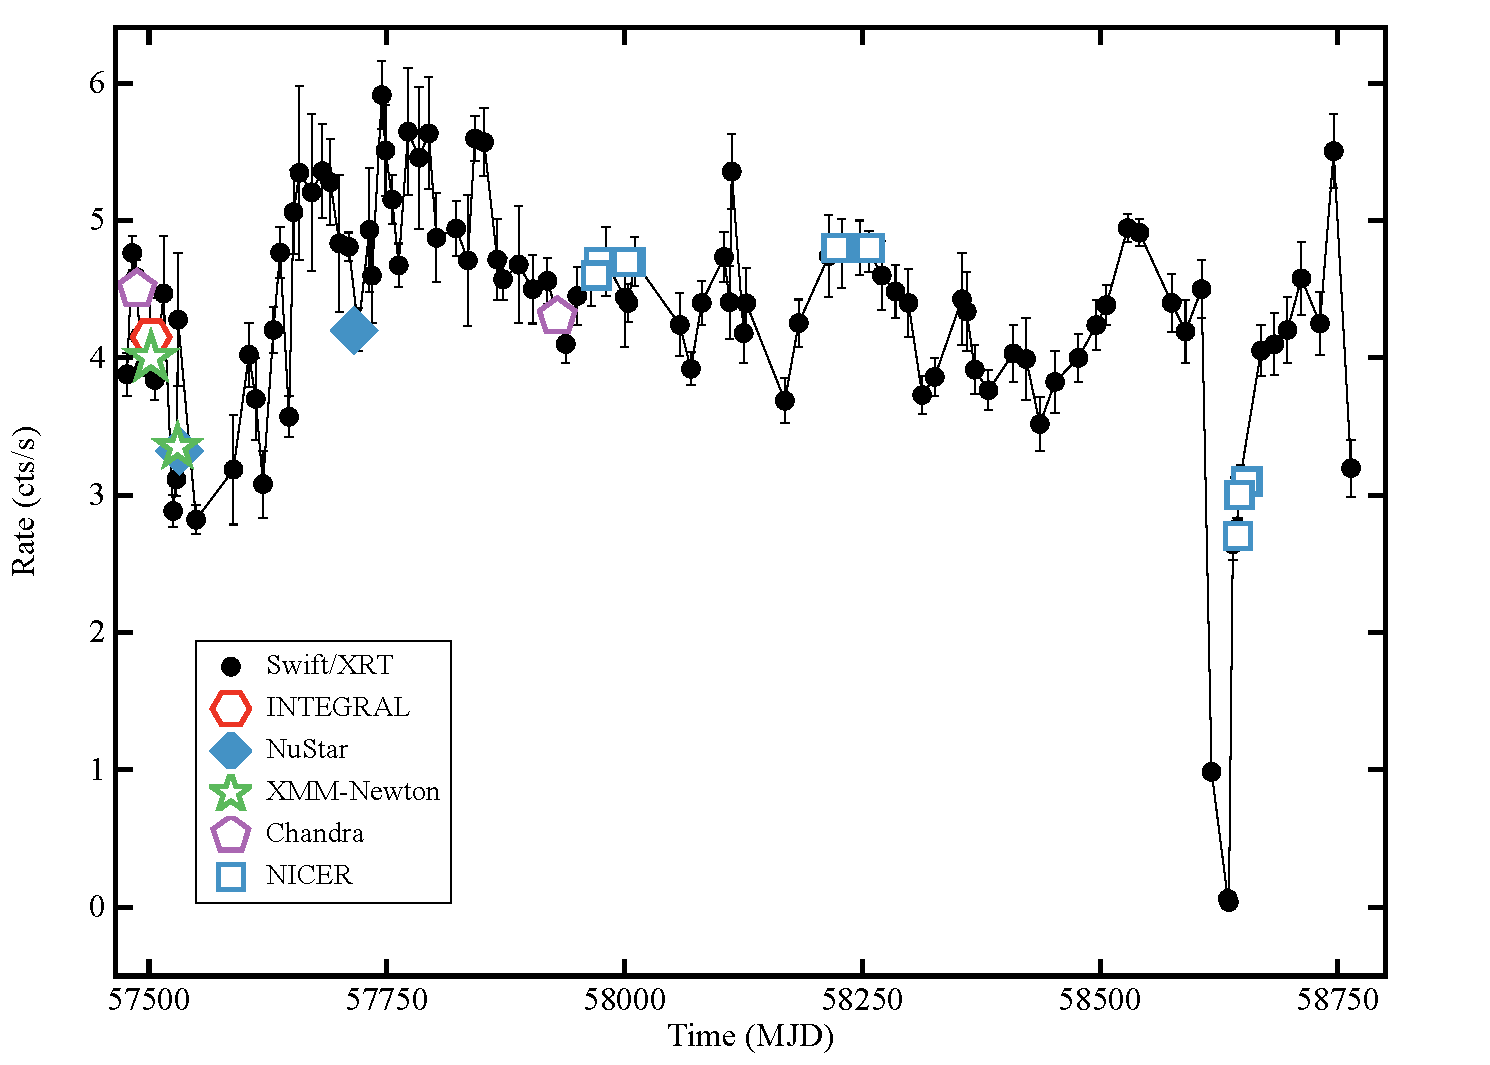
\includegraphics[width=0.55\textwidth]{REVIEW_AMXP/lc_updated_maxi_0911.pdf}
  \caption{MAXI J0911-655 light curve as observed by \swiftxrt{} (black points) since its discovery at the beginning of 2016. Green stars, blue diamonds, red hexagon, purple pentagons and blue squares represent the observations collected by \xmm{}, \nustar{}, \inte{}, \chandra{} and \nicer{} respectively. [Figure from \cite{Sanna2017a}}     
  \label{fig:lc_0911}
\end{figure}


Fig.~\ref{fig:lc_0911} shows the long-term monitoring of the source performed with \swiftxrt{} (black points) since its discovery on early 2016. Overlaid in the figure are also shown the source observations performed with X-ray facilities such as \xmm{}, \nustar{}, \inte{}, \chandra{} and \nicer{} performed during the last $\sim3.5$ years of uninterrupted outburst. We note that recently the source underwent an anomalous swing in luminosity, with the flux dropping from a \swiftxrt{} count rate of $~4.5$ cts/s to almost zero within a couple of weeks period, before returning to a high flux level \cite{Bult2019b}. The ongoing long-lasting X-ray outburst resembles the activity of the AMXP HETE J1900.1-2455, that underwent a long-lasting (about 10 years) active state. 
Interestingly, similarly to HETE J1900.1-2455, MAXI J0911-655 showed pulsations only during the first two months from its discovery \cite{Sanna2017a}.

Based on the mass function $f(m_2, m_1, i) \sim 6.2\times10^{-6}$ M$_\odot$, and the lack of eclipses (as well as dips) in the light curves, a minimum companion mass of $2.4\times 10^{-2}$ M$_\odot$ for a canonical 1.4 M$_\odot$ NS has been estimated. The Roche-lobe of the companion star could either be filled by a hot ($5\times10^{6}$ K) pure helium white dwarf with a $2.8\times 10^{-2}$ M$_\odot$ mass (implying an inclination angle $i\simeq 58^\circ$) or an old ($>5$ Gyr) brown dwarf with metallicity abundances between solar/sub-solar and mass ranging in the interval $6.5\times 10^{-2}$ and $8.5\times 10^{-2}$ M$_\odot$ ($16 < i < 21$). 

Finally, the broad-band energy spectra of MAXI J0911-655 is well described by the superposition of a weak soft black-body-like component (kT$\sim0.5$ keV) and a hard high-energy cut-off power-law ($\Gamma \sim 1.7$ and kTe $\sim130$ keV), in agreement with spectral properties of other AMXPs observed in a hard state \cite{Falanga2005a,Falanga2005b,Gierlinski2005,Patruno2009, Papitto2009,Papitto2009,Papitto2013a}. Moreover, the source shows marginal evidence of a weak and narrow reflection component in the energy range 6.5-6.6 keV which has been identifies as the K$\alpha$ emission line from helium-like iron \cite{Sanna2017a}.

Nearly-simultaneous radio and X-ray observations of the source performed by ATCA on April 6, 2016, failed to detect a radio counterpart \cite{Tudor2016}.


\subsection{IGR J17062-6143}

IGR J17062-6143, observed for the first time in 2006 by the \inte{} observatory \cite{Churazov2007}, it has been persistently accreting at luminosities in the range $\sim10^{-3}$ and $10^{-2}$ L$_\text{Edd}$ since then. The detection of Type-I X-ray bursts \cite{Degenaar2013} revealed the NS nature of the primary star, and it allowed to constrain the distance to 7.3$\pm$0.5 kpc \cite{Keek2017}.
X-ray pulsations at $\sim$163.6 Hz (fractional pulsed amplitude of $9.4\pm1.1$) have been detected in a single $\simeq 1200$ seconds observation with \rxte{} \cite{Strohmayer2017}, however, extensive pulsation search using the \xmm{} EPIC timing mode data of the source, did not confirm them.
Between August 9 and August 15 2017, the \nicer{} observatory observed IGR J17062-6143 for a total exposure of 26 ks confirming that the source is a $\sim$163.6 Hz pulsar, and also revealing an ultra-compact orbit. Phase coherent timing analysis of the \nicer{} data revealed an orbital period of $\sim38$ minutes, the shortest currently known for an AMXP, and a projected semi-major axis of $\sim4\times10^{-3}$ lt-s \cite{Strohmayer2018}.  

Variable detection of the coherent pulsation suggest that IGR J17062-6143 might be an intermittent AMXP. These sources, of which four other candidates are currently known (SAX J1748-2021 \cite{Altamirano2008,Sanna2016}, Aql X-1 \cite{Casella2008}, HETE J1900.1-2455 \cite{Kaaret2006} and MAXI J0911-655 \cite{Sanna2017a}, only show detectable pulsations a fraction of the time. In HETE J1900.1-2455, the pulsations disappeared around 2 months into the outbursts, only to sporadically reappear afterwards \cite{Patruno2012a} before the source returned to quiescence over a decade later \cite{Degenaar2017b}. Very similarly, MAXI J0911-655, showed pulsations for a few months from the beginning of the outburst, while none has been reported for the last 3 years of activity. Mechanisms such as accretion induced magnetic field burial has been proposed to explain the disappearance of the pulsations (see e.g. \cite{Cumming2001}, however, no definitive consensus has been reached on the subject. 

The NS mass function, $f_x=9.12\times 10^ {-8}$ M$_\odot$ defines a lower limit to the mass of the secondary star, $m_2$ in the range 0.005-0.007 M$_\odot$ for a NS mass in $m_1$=1.2-2 M$_\odot$ \cite{Strohmayer2018}. The constraints summarised in Fig.~\ref{fig:17062_mass} suggest that IGR J17062-6143
is observed at relatively low inclination, and the secondary appear to be consistent with the helium donors of AM CVn systems explored by \cite{Deloye2007} (
dotted curves in Fig.~\ref{fig:17062_mass}).

\begin{figure}
\centering
  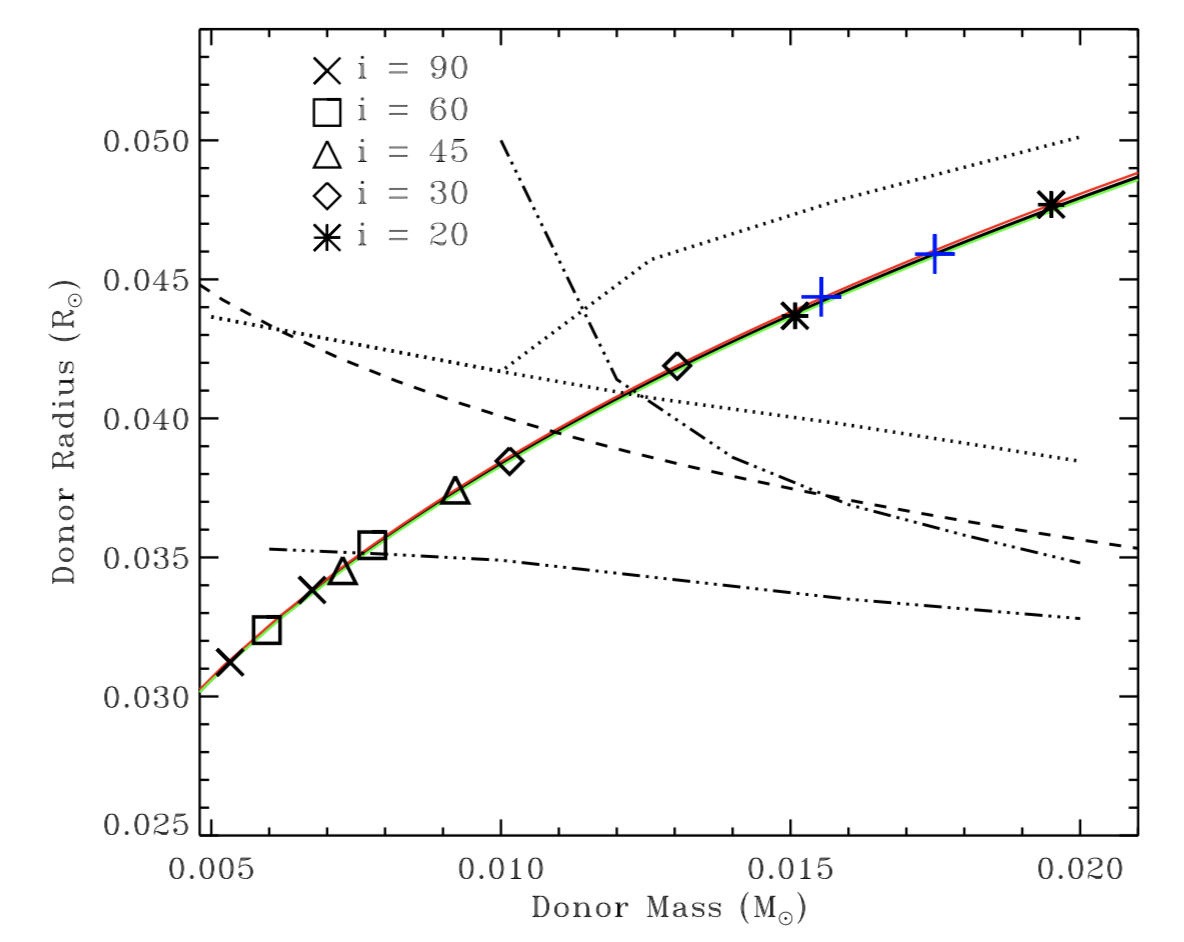
\includegraphics[width=0.55\textwidth]{REVIEW_AMXP/17062_donor_Strohmayer_2018.png}
  \caption{Constraints on the companion star in IGR J17062-6143. The Roche lobe constraint is plotted for three different NS masses, 1.2 (green), 1.4 (black), and
1.8 M$_\odot$ (red). The different symbols along the curves denote the secondary masses
from the mass function constraint for different assumed inclinations, $i$, and for
two values of the NS mass at each inclination. The dashed curve is the fitting formula from \cite{Nelemans2001} that approximates the mass-radius relation for low-mass, cold,
pure helium white dwarfs \cite{Zapolsky1969}. The dotted curves
denote a range of mass-radius values from the binary evolutionary calculations of \cite{Deloye2007} for the helium donors of AM CVn systems. The
dashed-dotted curves show mass-radius relations for carbon white dwarfs with
central temperatures of $10^4$ (lower) and $3\times10^6$ K (upper), from \cite{Deloye2003}. (Figure from \cite{Strohmayer2018}})     
  \label{fig:17062_mass}
\end{figure}
A hint for accretion from a degenerate helium dwarf in an ultra-compact system has been suggested from the properties of these long-duration (tens of minutes) thermonuclear X-ray bursts observed by \swiftxrt{} in 2015, consistent with the accumulation of
helium-rich material on the NS surface \cite{Keek2017}. However, accretion of hydrogen-rich fuel under certain conditions can also lead to thick, combustible helium layers, making helium-powered nuclear flashes not necessarily a definitive indication of a degenerate helium dwarf companion \cite{Fujimoto1981,Galloway2006}. 
 

The spectral properties of the source have been extensively investigated by \swift{}, \nustar{}, \chandra{}, and \xmm{}. \cite{Degenaar2017} reported the presence of Fe $K\alpha$ reflection features in the \nustar{} data, from which an inner disk truncated out to $\sim100$ gravitational radii can be inferred. Simultaneous \nustar{} and \xmm{} observations \cite{VandenEijnden2018}. They also report the presence of reflection features, suggesting a similarly truncated disk as in \cite{Degenaar2017}. They note, however, that a disk extending down to the NS surface cannot be excluded if the binary inclination is very low. Based on analysis of \xmm{} Reflection Grating Spectrometer data they also suggest that the system may have an oxygen-rich circumbinary environment, perhaps due to an outflow.

Multiwavelength analysis of IGR J17062-6143 have been carried out, showing that UV to NIR spectral energy distribution (SED) can be very well described by a standard accretion disc with outer radius of $\sim2.2\times10^{10}$ cm \cite{HernandezSantisteban2019}. Moreover, the SED modelling demonstrates that accretion disc spectrum does not extend into the soft X-rays implying that the thermal emission component seen in the X-ray spectrum of IGR J17062-6143 (and other NS LMXBs accreting at low rates) is likely from the surface of the NS, as was previously hypothesised based on X-ray spectral analysis (e.g. \cite{ArmasPadilla2013,Degenaar2017}. Studies of the low-resolution optical spectrum of the source show a blue-continuum consistent with an accretion disc, but no emission lines of H, He, or other elements are observed that do not allow to directly constrain the donor type.

\subsection{IGR J16597-3704}

IGR J16597-3704 is a transient LMXB discovered by \inte{} on October 2017 \cite{Bozzo2017} and located within the globular cluster NGC 6256 at a distance of roughly 9.1 kpc. Follow-up radio (VLA; \cite{Tetarenko2017}) and X-ray (\chandra{}; \cite{Chakrabarty2017}) observations provided accurate coordinates for the source. 
A \nustar{} observation performed a few days after the discovery of the source revealed X-ray pulsations at $\sim 105$ Hz characterised by a clear Doppler modulation compatible with a binary system of $\sim$46 minutes orbital period and projected semi-major axis of $\sim5$ lt-ms \cite{Sanna2018a}. Its short orbital period classifies IGR J16597-3704 among the so-called ultra-compact LMXBs. 

The system mass function $f(m_2 ,m_1 ,i)\sim 1.2\times 10^{-7}$ M$_\odot$ and the lack of eclipses/dips in the X-ray light curve of the source suggest a secondary mass $m_2\gtrsim6.5\times 10^{-3}$ M$_\odot$ ($m_2\gtrsim8\times 10^{-3}$ M$_\odot$) for a 1.4M$_\odot$ (2M$_
\odot$)NS, consistent with the expected donor mass of $\sim0.01$ M$_\odot$ for an ultra-compact NS binary in a 46-minute orbital period (e.g. \cite{vanHaaften2012}). Considerations on the pulsar spin equilibrium suggest a dipolar magnetic field of $9.2\times 10^{8} < B < 5.2\times 10^{10}$ G, significantly larger than the average magnetic field of known AMXPs (see e.g. \cite{Mukherjee2015, Degenaar2017}). Combined with the higher-than-average spin period of the source, this magnetic field suggests that IGR J16597-3704 has been discovered in a relatively early stage of its recycling process. \cite{Sanna2018a} note that the mass required to spin-up an old slowly-rotating NS up to $\sim105$ Hz (of the order of $10^{-3}$ M$_\odot$; see also \cite{Burderi1999} does not efficiently suppress the dipolar magnetic field, which limits the NS spin period.
Interestingly, the best pulse profile obtained epoch-folding the $\sim40$ ks \nustar{} observation (see Fig.~\ref{fig:16597} corrected for the updated ephemeris, it is harmonically reach with a peculiar pulse shape well fitted with a combination of four sinusoidal components, where the fundamental, second, third and fourth harmonics have fractional amplitudes of $\sim$14\%, $\sim$4\%, $\sim$3.8\% and $\sim$0.9\%, respectively. 
\begin{figure}
\centering
  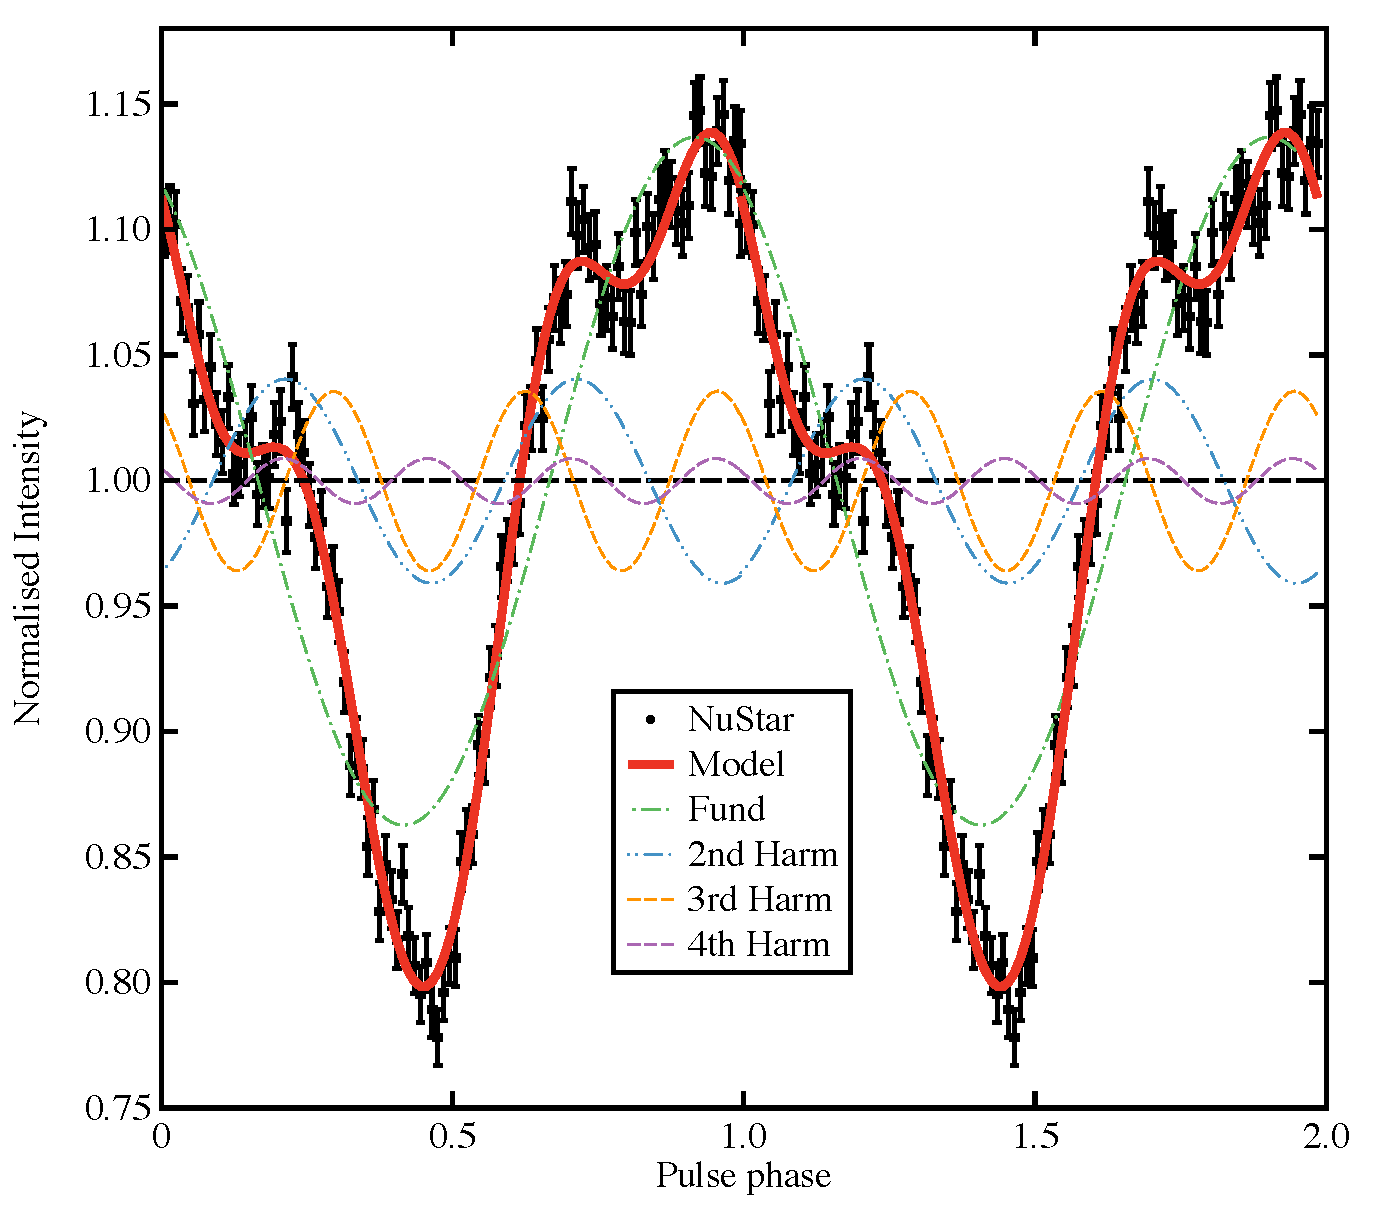
\includegraphics[width=0.49\textwidth]{REVIEW_AMXP/pulse_profile_nustar_latest2.pdf}
  \caption{IGR J16597-3704 pulse profile (black points) obtained from the epoch-folded \nustar{} data. The best fit model obtained by combining four sinusoidal components with harmonically related periods is also shown (red line).  
Two cycles of the pulse profile are shown for clarity. (Image taken from \cite{Sanna2018a}}     
\label{fig:16597}
\end{figure}

The energy spectrum of IGR J16597-3704 is  well-described by an absorbed disk blackbody ($k_T=1.42\pm0.07$ keV) plus thermally comptonized continuum ($\Gamma=2.3\pm0.2$) with seed 
photons from the blackbody ($k_{bb}=2.6\pm0.1$) radiation. The measured absorption column density 
of $(8.2\pm1.0)\times10^{21}$~cm$^{-2}$ is consistent with that expected in the direction of the source ($\sim 9.5\times10^{21}$ cm$^{-2}$) using the cluster A$_V$ \cite{Harris1996} and the appropriate conversion from A$_V$ to N$_H$ assuming Wilms abundances (see e.g. \cite{Bahramian2015,Foight2016}). No evidence for spectral lines (e.g. Iron K-$\alpha$) or reflection humps has been reported \cite{Sanna2018b}.

Interestingly, the large magnetic field combined with the moderately long spin period could be also responsible for the structured pulse profile, as well as the lack of emission lines and reflection components in the energy spectrum.

Radio counterpart to IGR J16597-3704 was observed by the VLA facility between 2017 October 23 and 27. The radio observations revealed that IGR J16597-3704 is one of the more radio faint systems in the NS X-ray binary population. Moreover, on 2017 November 3 the source was observed at the Parkes radio telescope with the aim of searching for radio pulsations. No radio pulsation were found down to a flux density of 0.05 mJy.

\subsection{IGR J17379-3747}

The X-ray transient IGR J17379-3747 was first discovered on February 2004 through the detection of a type I X-ray burst with \inte{} \cite{Chelovekov2006}. An independent classification was obtained later on with \rxte{} \cite{Markwardt2008}, while the source was ultimately catalogued after the \swiftxrt{} X-ray localization \cite{Bird2007,Krivonos2007,Krimm2008}. Archival \inte{} and \rxte{} observations suggest that the 2004 outburst of the source lasted for almost 40 days \cite{Markwardt2008,Chelovekov2010}. On September 2008, \rxte{} revealed a second outburst of the source characterised by a gradual decline in flux, with the total outburst lasting roughly 2-3 weeks \cite{Markwardt2008,Shaw2008}.
Renewed activity from the source was detected by \maxigsc{} on March 2018 \cite{Negoro2018}. Follow-up observations with \nicer{} and \xmm{} allowed the discovery of 468 Hz coherent X-ray pulsations \cite{Strohmayer2018b,Sanna2018b}. Analysis of the archival \rxte{} data led to recover pulse detections in both previous outbursts \cite{Sanna2018b}.
The source distance is still not precisely determined, however, based on its location in the direction of the Galactic center an assumed distance of 8.5 kpc is typically adopted. 

The binary system mass function $f(m_2 , m_1 , i) \sim 8\times 10^{-5}$ M$_{\odot}$ as well as the lack of eclipses (inclination angle of $i<75^\circ$ ) in the X-ray light curve, suggests a donor mass $m_2 < 0.056$ M$_\odot$ for a 1.4 M$_\odot$ NS ($m_2< 0.07$ M$_\odot$ for a 2 M$_\odot$ NS). Considerations on the binary mass transfer conditions suggest that the companion star could be a hot brown dwarf, likely heated by low-level X-ray radiation during the quiescent phases (e.g. \cite{Sanna2018b,Bildsten2001,Galloway2005b}). 

The 0.5-10 keV average energy spectrum of IGR J17379-3747 is well described by a superposition of a soft disk component (kT$\sim$0.45keV) and a hard power law ($\Gamma\sim1.9$), consistent with typical AMXPs observed in outburst (see e.g \cite{Gierlinski2005,Papitto2009,Falanga2012}). No evidence of emission lines or reflection components in the energy spectrum have been reported \cite{Sanna2018b}, in analogy with the AMXPs XTE J1807-294 \cite{Falanga2005a}, XTE J1751-305 \cite{Miller2003}, SWIFT J1756.9-2508 \cite{Sanna2018d}, and IGR J16597-3704 
\cite{Sanna2018a}. 

The dipolar magnetic field $B$ has been constrained between $0.4\times 10^{8}$ G and $2.3\times 10^{9}$ G assuming accretion-torque equilibrium in combination with the source luminosity extrapolated from the latest outburst. The value of $B$ is consistent with the average magnetic field of known AMXPs (see e.g. \cite{Mukherjee2015,Degenaar2017}).

Coherent pulsation at $\sim 468$ Hz shows clear Doppler modulation compatible with the NS being part of a binary system with orbital period of $\sim$ 1.9 hours and a projected semi-major axis of $\sim8$ lt-ms. Combining the barycentric spin frequency values observed in the three observed outbursts, it has been estimated an upper limit (3$\sigma$ confidence level) of the secular spin derivative $-8.3\times 10^{-13}$< $\dot{\nu}< 1.1\times 10^{-12}$ Hz s$^{-1}$, corresponding to an upper limit on the magnetic field strength of $B < 2.8\times 10^{9}$ G (assuming a NS R = 10 km and an angle $\alpha\simeq20^{\circ}$ between the magnetic hotspot and the rotational pole), consistent with the estimate obtained from the dynamics of the NS in accretion \cite{Sanna2018b}.
Finally, an update valued of the binary orbital period has been estimated by investigating the orbital period secular evolution of the source through the ephemeris of the three observed outbursts of the source, obtaining a more accurate value of the orbital period Porb = 6765.84521(2) s and an orbital period derivative $\dot{P}_{orb} = (-2.5\pm 2.3)\times 10^{-12}$ s s$^{-1}$.

IGR J17379-3747 was observed by VLA on March 2018, at 4.5 and 7.5 GHz (each with a bandwidth of 1 GHz) simultaneously. A flat-spectrum radio counterpart with a flux density of $\simeq0.4$mJy at 4.5 and 7.5 GHz at a position consistent with the X-ray source (see e.g. \cite{vandenEijnden2018b}). 

\subsection{IGR J17591-2342}
The source \igrsev{} was discovered by \ibis{} on board the \inte{} satellite on August 10, 2018. Trigger by the discovery of the source, \swift{}, \nustar{} and \nicer{} observed the source leading to the detection of coherent X-ray pulsations at $\sim$527 Hz \cite{Sanna2018c}. The NS spin frequency showed a clear drift compatible with a Doppler shift induced by the binary orbital motion with period close to 8.8 hours, very similar to the intermittent AMXP SAX J1748.9-2021 \cite{Altamirano2008} and the eclipsing AMXP SWIFT J1749.4-2807 \cite{Markwardt2010b,Altamirano2011, Ferrigno2011}.

The mass function $f(m_2, m_1, i)\sim1.5 \times 10^{-2}$~M$_{\odot}$ of \igrsev{} implies a minimum companion mass of $m_2=0.37$~M$_{\odot}$ (for a 1.4~M$_{\odot}$ NS and binary inclination $i=90^{\circ}$). Since neither total eclipses nor dips have been observed in the X-ray light curves, the binary inclination can be limited to values lower than 60 degrees %$i \lesssim 60^{\circ}$ 
\cite{Frank2002}, for which a lower limit $m_2 \gtrsim $0.42~M$_{\odot}$ can be inferred (for a 1.4~M$_{\odot}$ NS). The value increases up to $m_2 \gtrsim 0.52$~M$_{\odot}$ if we consider a 2~M$_{\odot}$ NS. 

A comparison between mass-radius relation of the donor star obtained from the Roche-lobe overflow condition (see e.g. \cite{Sanna2018c}) and numerically simulated mass-radius relations for zero-age main-sequence stars (ZAMS; \cite{Tout1996}), as well as isochrones for stars of 8 and 12\,Gyr \cite{Girardi2000}, suggest that the companion star is compatible with either a ZAMS with mass $\sim1.1$ M$_\odot$ (corresponding to an inclination angle of $i\sim24$ degrees) or an old main-sequence star with mass 0.85$-$0.92 M$_\odot$ ($i$ ranging between $28$ and $30$ degrees) for a stellar age between 8 and 12\,Gyr. It should be noted, however, that the \textit{\textup{a priori}} probability of observing a binary system with inclination $i\leq 30$ degrees is of the order of 13\%. Nonetheless, it should not be excluded the possibility of a bloated donor star with the limitation that its thermal timescale ($GM^2_c/R_c L_c$) should be much longer than the evolutionary timescale ($M_c/\dot{M_c}$).


Phase-coherent timing analysis of the \nicer{} observations performed between August 15 and August 24, revealed a spin-up frequency derivative of (2.0$\pm$1.6)$\times 10^{-13}$\,Hz/s. 
This values is compatible with the maximum spin-up derivative estimated under the assumption of accretion of matter leaving the accretion disc with angular momentum equal to that at the co-rotation radius, and mass accretion rate of $\dot{M}\simeq5.2\times10^{-10}$ M$_{\odot}$/yr (for an NS radius and mass of 1.4\,M$_{\odot}$ and 10 km) obtained for a broad-band (0.1--100 keV) absorbed flux of $\sim7\times10^{-10}$ erg/s/cm$^2$ and a source distance of 8.5 kpc (assumed near the Galactic centre, see, e.g. \cite{Kerr1986}).
However, increasing the analysis baseline of the outburst (between August 15 and October 15) seems to suggest a spin-down frequency derivative of (-7.4$\pm$0.3)$\times 10^{-14}$\,Hz/s (Sanna et al. 2020 in prep.). 


The NS dipolar magnetic field can be roughly constrained in the range $1.4\times10^8<B<8\times 10^{9}$ G by assuming the condition of spin equilibrium for accreting X-ray pulsars. This value is consistent with the average magnetic field of known AMXPs \cite{Mukherjee2015}. 


Finally, the broad-band energy spectrum (0.5-80 keV) of \igrsev{}, obtained combining almost simultaneous \swift{}, \nustar{} and \inte{} observations, is well described by an absorbed soft black-body-like component ($kT\sim 0.8$ keV) with a relatively small emitting area that is compatible with emission from the NS surface (or part of it) plus a Comptonised component ($\Gamma \sim 1.8$) with a seed photon temperature compatible with the soft thermal component. The spectral properties of the source are consistent with those of other AMXPs observed in the hard state \cite{Falanga2005a,Gierlinski2005,Papitto2009, Papitto2013a,Sanna2017d,Sanna2017b}. Marginal evidence of a weak emission line compatible with the iron K-$\alpha$ transition are present, in accordance with other AMXPs in the same accretion state \cite{Sanna2017d,Sanna2017b}.
\end{comment}


%\section{}
% Always give a unique label
% and use \ref{<label>} for cross-references
% and \cite{<label>} for bibliographic references
% use \sectionmark{}
% to alter or adjust the section heading in the running head



\bibliographystyle{spmpsci.bst}
\bibliography{export-bibtex.bib}

\end{document}


